\documentclass[oneside, single, authoryear, semicolon, 12pt]{lion-msc}
\usepackage{lipsum}
\usepackage{booktabs}
\usepackage{pifont}
\usepackage[version=4]{mhchem}
\usepackage{parskip}
\usepackage{float}
\usepackage{makecell}
\usepackage{graphicx}
\usepackage{subcaption}
\usepackage{caption} 
\usepackage{amsmath}
\usepackage{amssymb}
\title{Detecting Nitrogen Carriers in Planet-Forming Regions of Protoplanetary Disks}
\author{Niels de Klerk}

\major{Astronomy and Physics}
\affiliation{Leiden Observatory, Universiteit Leiden}

\newdate{date}{\day}{\month}{\year}           % definition of time and date using datetime package
% \newdate{date}{27}{08}{2010}
\date{\displaydate{date}}

\studentid{s3640477}                           % check you student ID, LaTeX does not do this
\abstract{Nitrogen is one of the most important elements for life on Earth, as it is a component of molecules, like amino acids, and proteins.\ In addition, it plays an important role in the chemistry of protoplanetary disks, which are the birthplace for planets. Several molecules containing nitrogen were detected in disks, such as CN, NO, and HCN, using ALMA. However, the only nitrogen carrier detected in the IR is HCN. This thesis aims to investigate the possibility of detecting NO and NH\3 in protoplanetary disks using spectra taken by JWST MIRI MRS. For this, a grid of ProDiMo models with varying C and O abundances is used in combination with FLiTs to create spectra. We investigated the effects of the C and O abundances on the flux and selected spectral regions of interest. Furthermore, a technique of detecting molecules using cross-correlation is studied. Utilizing this technique, molecules already detected in GWLup, Sz98, and V1094Sco are reaffirmed, with a possible first detection in IR of NO in V1094Sco. We used LTE models to set upper limits on the column densities of NO and NH\3 for GWLup, Sz98, and V1094Sco.}% limit your self to 1/2 page or 500 words
\dailysupervisor{Marissa Vlasblom, Msc.  \\ \hspace*{\fill}Aditya M. Arabhavi, Msc.}
\supervisor{Prof. Dr. Ewine van Dishoeck \\ \hspace*{\fill}Prof. Dr. Inga Kamp} % Note that this should be a LION staff member!
\corrector{Dr. Matthieu Schaller}                      % This could be a LION staff member or your external supervisor

\degree{Bachelor of Science}                     % The default option is "Bachelor of Science", change if needed

\major{Astronomy and Physics}                  % The default option is "Physics", change if needed
%\major{Physics and Mathematics}

% optional cover picture - should be jpg or pdf
% \coverpicture{
\includegraphics[width=2cm]{Latex/lion-msc-logo.pdf}}

% Use this to make hyperlinks visible in the document.
\hypersetup{colorlinks=true}

% ---------------------------------------------------------------- My defintions!
\renewcommand{\vec}[1] {\ensuremath{ \overrightarrow{ #1 } }}
% \renewcommand{\vec}[1] {\ensuremath{ \mathbf{ #1 } }}
% \bra \ket \braket and \proj
\newcommand{\bra}[1]{\ensuremath{\langle #1 \vert}}
\newcommand{\ket}[1]{\ensuremath{\vert #1 \rangle}}
\newcommand{\braket}[2]{\ensuremath{\langle #1 \vert #2 \rangle}}
\newcommand{\proj}[1]{\ensuremath{\vert #1 \rangle \langle #1 \vert}}

\newcommand{\kpar}{\ensuremath{k_\parallel}}

\newcommand{\4}{$_4$}
\newcommand{\3}{$_3$}
\newcommand{\2}{$_2$}
% ----------------------------------------------------------------

% \usepackage{tocloft}
% \renewcommand{\cftchapdotsep}{\cftdotsep}
\begin{document}

% roman numbering in the table of contents section
\pagenumbering{roman}

\maketitle

% Table of contents:  it is a good idea to include this into your thesis
\tableofcontents
\cleardoublepage
\pagenumbering{arabic}
\chapter{Introduction}
The nebular hypothesis states that a planetary system is formed from a slowly rotating molecular cloud that collapses into a disk. This theory was first proposed in \textit{The Principia} by Emanuel Swedenborg in 1745. Immanuel Kant developed the theory further in 1752 and was later modified by Pierre-Simon Laplace in 1796. Centuries later, the first protoplanetary disk was observed by O'Dell using the Hubble Space Telescope \citep{ODell1993}. In recent years, the Atacama Large Millimeter/submillimeter Array (ALMA) has imaged a large collection of these protoplanetary disks, showing a wide variety of structures and compositions (e.g. \cite{Andrews_2018, ALMA2015}). Furthermore, the James Webb Space Telescope (JWST) has provided new insight into protoplanetary disks. For example, the JWST Mid-InfraRed Instrument (MIRI) mid-INfrared Disk Survey (MINDS) team uses the JWST to investigate the inner parts of protoplanetary disks (e.g. \cite{Kamp_2023, henning2024mindsjwstmirimidinfrared}). The study of protoplanetary disks is important to find answers to the fundamental question: 'How did life arise?' and 'Are we alone in the universe?'.

The spectrum of protoplanetary disks can tell us a lot about the properties of the disk and the host star. An important example is the observation of the disk around a T Tauri star Sz98 \citep{Gasman_2023}. Using MIRI MRS on the JWST, they probed the inner regions of the disk. They detected CO$_2$, H$_2$O, OH, CO, and HCN. Furthermore, no other organics were detected, suggesting a low C/O ($<$0.5) ratio. This result differed from the ratio found using ALMA ($>$1), which probed the outer regions. This highlights the complexity of disks and their chemistry.

However, this observation is not necessarily representative of disks. \cite{colmenares2024jwstmiridetectioncarbonrichchemistry} observed a disk around the T Tauri star DoAr 33 with an exceptionally high C/O ratio of 2-4. In addition to CO, H\2O, and CO\2, like in the Sz98 disk, the more complex carbohydrates C\2H\2 and C\4H\2 were found. The presence of these molecules is indicative of this high ratio. A possible explanation for this carbon-rich environment is the slow accretion rate of the star, which slows the radial mixing and the persistence of the carbon-grain destruction.

\cite{Grant_2023} observed the protoplanetary disk around the T Tauri star GW Lup and reported the first detection of $^{13}$CO$_2$ in a protoplanetary disk. The combination of the spectral resolution of the JWST-MIRI and the high SNR allows for the detection of weaker spectral features. Notably, the deduced N$_{CO_2}$/N$_{H_2O}$ was significantly higher than previously thought. This could indicate a cavity between the H$_2$O and CO$_2$ snowlines. These findings demonstrate the new possibilities that JWST offers for studying disk structures. 

However, there have been no detections of nitrogen carriers other than HCN in IR. Nitrogen carriers have been detected in protoplanetary disks in different parts of the electromagnetic spectrum. For example, \cite{Salinas_2016} detected the first NH\3 in a protoplanetary disk using the Herschel Wide Band Spectrometer (WBS). WBS observes in the radio part of the electromagnetic spectrum. The inferred column density of NH\3 varies by orders of magnitude depending on the assumed geometry of the water vapor in the disk. They stress the importance of high spatial resolution to constrain the column densities of NH\3.

Another example is the first detection of NO in a protoplanetary disk by \cite{firstnodetect}. They observed the disk using ALMA (radio). They implemented DALI to model the column density of NO. Their model prediction aligns with the observation of the north side of the disk. However, their model underpredicts the NO column density on the south side of the disk, where a dust trap is located. Other molecules, like N\2O and HNCO, could explain the difference. This study exemplifies the importance of dust traps for the chemistry in the disk and proposes to use CN and NO as tracers of the C/O ratio.

NH\3 has been detected using JWST MIRI MRS in an object closely related to protoplanetary, namely a protostar, by \cite{van_Gelder_2024}. As part of the JWST Observations of Young protoStars (JOYS), they observed 18 low-mass protostar systems. Along with detection from common detection, such as H\2O and CO\2, they detected SiO, CN, and NH\3 for the first time in protostars, highlighting the power of JWST to detect volatile molecules in the early stages of star formation.

In this thesis, we investigate the possibility of detecting NO and NH\3 in protoplanetary disks using spectra taken by JWST MIRI MRS. First, we examine how nitrogen carriers depend on the abundances of carbon and oxygen. Next, we develop a method to detect nitric oxide (NO) and ammonia (NH\3) in the spectra of protoplanetary disks using JWST MIRI MRS. Lastly, we apply our methods to observations and determine upper limits on the column densities of NO and NH\3 for these sources. The theory behind protoplanetary disks and spectroscopy is explained in \autoref{Ch: theory}. We present the model's setup and the cross-correlation technique in \autoref{Ch: Methods}. The output of the model simulation and the application of the cross-correlation technique are shown in \autoref{Ch: Results}. We discuss the results and their implications in \autoref{Ch: Discussion}. In \autoref{Ch: Conclusions}, we conclude our thesis.

\chapter{Theoretical Background}\label{Ch: theory}
\section{Formation and Evolution of Protoplanetary Disks}
Protoplanetary disks are collections of gas and dust that surround protostars. Their formation and evolution are closely tied to that of their host star. This section discusses how protoplanetary disks form, their evolution, the formation of substructures and planets, and the ultimate end of disks. 

\subsection{Formation of Disks}
Molecular clouds are large collections of gas and dust. When these clouds are perturbed, parts of the cloud can become dense enough, resulting in the collapse under their own gravity \citep{1987ARA&A..25...23S}. This results in the creation of a protostar surrounded by gas and dust. The angular momentum of each of the particles is approximately randomly oriented, but on average, the angular momentum vector points in a certain direction. Two particles colliding cause them to exchange angular momentum. If many collisions happen, all the angular momenta other than the average angular momentum vector cancel out. This results in the formation of a protoplanetary disk around the protostar. Surrounding the protostar and the disk is the approximately spherically shaped envelope of material that did not get distorted due to rotation. The composition of the disks can be divided into gas and dust. Gas, in this case, refers to molecules that are in gaseous form (H\2, He, H\2O, etc.) with low densities. The gas makes up $\sim$99\% of the disk \citep{Diskcomp}. Solid particulates, which are made up of silicates, carbonaceous materials, and ices, make up the remaining $\sim$1\% in the disk as dust.

The evolution of the disk can be categorized into four classes \citep{1987ApJ...312..788A}. Class 0 objects have an optically thick envelope that surrounds the protostar. For class 0 objects, the disk is starting to form, but it is not yet visible. Class I objects have a star and disk but are still embedded in an optically thick envelope. The star and disk become visible in class II objects as the star has become bright enough to blow away the envelope via radiative pressure. In class III objects, the disk has largely been depleted of gas and dust, leaving behind planets and planetesimals. The evolution from molecular cloud to planetary system has been confirmed by observation (e.g. \cite{Furlan_2016, J_rgensen_2009}).

Protoplanetary disks are roughly shaped like flat circles, extending from the hot inner region ($<$ 0.1 au) through the mid disk to the cold outer disk ($>$ 100 au). Both the temperature and the density of the disk decrease with distance from the host star. Due to hydrostatic equilibrium, the height above the midplane increases with distance, making protoplanetary disks flared. This is the result of the balance of gravity, pulling the disk together, and thermal pressure, pushing it apart. As the temperature and density decrease with distance, this balance changes. The height of the disk can be roughly captured by the scale height

\begin{equation}
    H = \frac{c_s}{\Omega},
\end{equation}

where $c_s$ is the speed of sound, and $\Omega$ the orbital frequency \citep{chap1}. This is the height over which the density decreases by a factor $e$. 
Vertically, disks can be separated into three regions: the cold midplane, warm molecular layer, and the hot ionized surface. The midplane runs through the middle of the disk and is the coldest. In this region, the disk is mostly made up of ice and dust. In the warm molecular layer, the disk is mostly made up of gas, and in the hot ionized surface, the gas has become ionized due to exposure to radiation from the star.

\subsection{Disk Dynamics}
Protoplanetary disks are not stationary objects. Several effects, like viscosity, determine how the disk evolves \citep{chap1}. Material in the disk experiences the viscosity of the disk as it moves around. This causes it to lose angular momentum, moving it closer to the host star.

Magnetic fields act like springs between particles. When particles in adjacent orbits come close together, they can magnetically interact. These particles have different velocities, where the particle in the inner orbit has a larger speed than the particle in the outer orbit. The interaction between the particles will make their velocities more similar. As a result, the particle in the inner orbit loses angular momentum, and the particle in the outer orbit gains it. Therefore, the inner particle moves closer to the star and falls into an orbit with a higher speed, whereas the other particle does the opposite. Hence, the difference in velocity is increased, which means there is an instability. This instability is known as magneto-rotational instability (MRI), and was first described by \cite{RevModPhys.70.1}. 

The material in the disk approximately follows a Keplerian orbit. This means that the velocity $v \propto r^{-1/2}$ decreases with distance from its host star. Therefore, material in adjacent orbits moves at different velocities. This causes shearing forces, which result in turbulence and mixing of material \citep{chap1}.  

Dust particles move around in the protoplanetary disk. Due to their relative motion with the gas, they experience drag, slowing them down. This results in the radial drift of dust particles towards the star, where they ultimately accrete onto it. Furthermore, the drag causes settling towards the midplane of the disk. 

When protoplanetary disks reach a critical mass, they can collapse under their own gravity. This effect is counteracted by pressure gradients and shear motion as they oppose the inward force of gravity. All of these influences on the stability of the disk can be captured by the Toomre Q parameter \citep{1964ApJ...139.1217T}

\begin{equation}
    Q = \frac{c_\mathrm{s}\Omega}{\pi G\Sigma}
\end{equation}

where $G$ the gravitational constant, and $\Sigma$ the surface density. The disk is stable against gravity for $Q > 1$. However, the disk can fragment and form spirals and gaps when $Q < 1$. This results in material getting close together, which leads to planet formation.

\subsection{Planets and Substructures}

To form planets around a star, dust particles need to clump together. However, this process is slow as the size of the dust particles is on the order of micrometers, and planets are on the order of thousands of kilometers in size. Through collisions, particles can stick together to form bigger particles. However, there are several limiting factors that reduce this growth. As particles get bigger, they experience more drag, so they slow down greatly. This limits the number of collisions as the particle encounters fewer other particles. Another effect of the larger drag is the loss of angular momentum. This results in the inward drift of the pebbles, which accrete any pebbles on the star before they get larger. Another limitation is that when bigger particles collide, the collision can be so powerful that it breaks them up into tiny pieces. 

Gaps in the disk can form due to several reasons, like photoevaporation, but one notable reason is the interaction with a planet.

\subsection{Disk Dispersion}
Protoplanetary disks will lose their gas and dust over time via mechanisms like viscosity, disk-planet interactions, and high-energy radiation.

Due to the viscosity of the disk, gas and dust lose angular momentum, which is transported outward. Eventually, they end up falling into the host star and depleting the disk of their material. 

The formation of planets also takes up material from the disk. Rings can form in the disk as planets open gaps due to tidal interactions, taking up the material in the regions. \textbf{Pebble and gas accretion}

Moreover, high-energy radiation from the host star heats material to temperatures higher than the escape velocity. That material is expelled from the system as a steady wind. 

Transition disks are a subset of protoplanetary disks that have a large inner gap. The gap is caused by the light of the star blowing away material. Gas is the first component that gets removed from the disk. This leaves behind the dust, forming a gas-poor debris disk. Protoplanetary disks are short-lived objects, only lasting 1-10 million years. 


\section{Disk Chemistry}
The chemistry in protoplanetary disks underpins the formation of all kinds of chemical compounds and ultimately determines the composition of planets.  However, it is extremely complex and involves a plethora of mechanisms and environmental factors. 

\subsection{Gas-Phase Chemistry}
Gas makes up the majority of the protoplanetary disks. This makes this part of the disk play an important role in the chemistry of the disk. The chemistry is highly dependent on the temperature and the density of the gas. For chemical reactions to take place, reactants need to come close together. As temperature increases, the average speed of the molecules also increases. This allows molecules to have more collisions, which means the reaction rate is higher. The same is true for higher densities, as this allows for more collisions as well. In the inner regions of protoplanetary disks, the temperature of the environment is higher due to the proximity of the star, resulting in more efficient chemistry. In the other regions, where the temperature is much lower, the chemistry slows down considerably. 

When a negatively charged ion, an anion, bonds with a neutral atom, it can emit an electron. This is called associative detachment. One of the most important examples of this process is the formation of molecular hydrogen from a neutral hydrogen atom and a negatively charged hydrogen atom (\ce{H + H- -> H2 + e-}). A similar process is radiative recombination, where a positively charged ion, a cation, absorbs an electron and emits a photon (e.g. \ce{H+ + e- -> H + h$\nu$}). Another process that moves the charge between atoms is charge-transfer reactions, where two atoms exchange an electron.

In the upper atmosphere of protoplanetary disks, gas is exposed to high-energy radiation, such as UV and X-rays. This leads to processes, like photodissociation and photoionization. In photodissociation, molecules get destroyed when they are hit by a high-energy photon (e.g. \ce{H2O + h$\nu$ -> OH + H }). For photoionization, the high-energy photon knocks an electron out of its orbital (e.g.  \ce{H + h$\nu$ -> H+ + e- }). These processes produce ions and radicals that go on to drive different chemistry. 

At larger distances from the star, the temperature goes down. When the temperature drops below the freezing point of a molecule, at a certain point, this is called the snowline. The snowlines depend on the molecules, as each molecule can have a different distance, thus temperature, at which it freezes out. For example, the CO\2 is farther out than the H\2O snowline \citep{vlasblom2023midinfraredspectrattauri}. At larger radii, the molecules are mostly in the solid phase on grains.  

\subsection{Grain-Surface Chemistry}
In the colder and denser regions of protoplanetary disks, chemistry takes place on the surfaces of grains.  The grains can act as the catalyst in chemical reactions. Molecules can stick to surfaces via adsorption, and beyond the snowline, molecules freeze out on the surface of grains, forming an ice layer. 

Molecules diffuse across the surface and react with other molecules. At relatively high temperatures, this is done by thermal hopping. There is an energy barrier that the molecules need to overcome to diffuse. When temperature fluctuations are high enough, some molecules can overcome the barrier. However, at very low temperatures, this is nearly impossible. To overcome the energy barrier, molecules must quantum tunnel. This still allows for chemistry to take place, even at low temperatures. 

Over time, increasingly complex molecules can form on the surfaces. In particular, complex organic molecules (COM) are interesting as they are possibly the origin of organic life. 

However, molecules on the surfaces of grains are not there forever. Several mechanisms cause the molecules to transition to the gas phase, i.e., desorption. When high-energy photons hit grains, they can photodesorb molecules off the grain's surface, but this can also result in photochemistry as discussed in the previous part. Photodesorption is dominant in the surface layers of the disk. Other mechanisms, such as thermal desorption and cosmic rays hitting the surface, can remove molecules from the grains and put them back in the gas. As a result, there is an interplay between gas and grain-surface chemistry, where they each affect the molecules that are being produced and destroyed.

\subsection{Chemical Networks}
A chemical network is made up of different types of molecules with connections between them. The connections represent reactions, such as the formation and destruction of molecules. 

Chemical network can be made up from hundreds to thousands of molecules. 

\textbf{MORE TEXT}

\newpage
\section{Emission Mechanisms}
Understanding how molecules emit photons is important, as this can help to understand how molecules are detected in spectra. In this section, we will explain how these processes work. This is largely based on Chapter 11 of \cite{1979rpa..book.....R}. 

When a molecule transitions from a higher energy state to a lower energy state, it emits a photon with a wavelength given by

\begin{equation}
    \lambda=\frac{hc}{\Delta E},
\end{equation}

where $\lambda$ is the wavelength of the light, $h$ the Planck constant, $c$ the speed of light, and $\Delta E$ is the difference in energy between the two states. Molecules order themselves in different energy states following the rules of thermodynamics. In thermal equilibrium, they organize according to the Boltzmann distribution 

\begin{equation}
    \frac{N_i}{N}=\frac{g_i\exp{(-E_i/k_\mathrm{B}T)}}{Z},
    \label{eq: boltzmann}
\end{equation}

with $N_i$ the number of molecules in state $i$, $N$ the total number of molecules $N=\sum_iN_i$, $E_i$ the energy of state $i$, $g_i$ the degeneracy of that energy state, $k_\mathrm{B}$ the Boltzmann constant, $T$ the temperature of the molecule and $Z$ the partition function $Z=\sum_j g_j\exp{(-E_j/k_\mathrm{B}T)}$.
Different transitions can take place within molecules. This section will discuss the three most fundamental transitions: electronic, vibrational, and rotational.

\subsection{Electronic Transition}
The transition with the highest energy is the electronic transition. In this transition, an electron jumps from an orbital with higher energy to one with lower energy. This reduces the total energy of the molecule. For simplicity, we will examine the hydrogen atom. The energy levels in the hydrogen atom are determined by

\begin{equation}
    E^e=-\frac{13.6\mathrm{ eV}}{n^2},
    \label{eq: electronic}
\end{equation}

where $n$ is the principal quantum number. The energy 13.6 eV in \autoref{eq: electronic} is called the ionization energy. This is the energy an electron in the ground state needs to gain to get unbound, resulting in the ionization of the atom. The transitions to $n=1$ are called the Lyman series (Ly$\alpha$, Ly$\beta$, etc.). The Balmer series corresponds with the transitions to $n=2$ (H$\alpha$, H$\beta$, etc) and the Paschen series (Pa$\alpha$, Pa$\beta$, etc) with $n=3$. For $n=4$, there is the Pfund series (Pf$\alpha$, Pf$\beta$, etc), and for $n=5$, the Humphreys series (Hu$\alpha$, Hu$\beta$, etc). Any other transitions do not have special names. The degeneracy of each state is $g(n)=2n^2$. The energy levels and the line strengths corresponding to transitions between these energy levels are shown in \autoref{fig: elec}.

\begin{figure}[H]
    \centering
    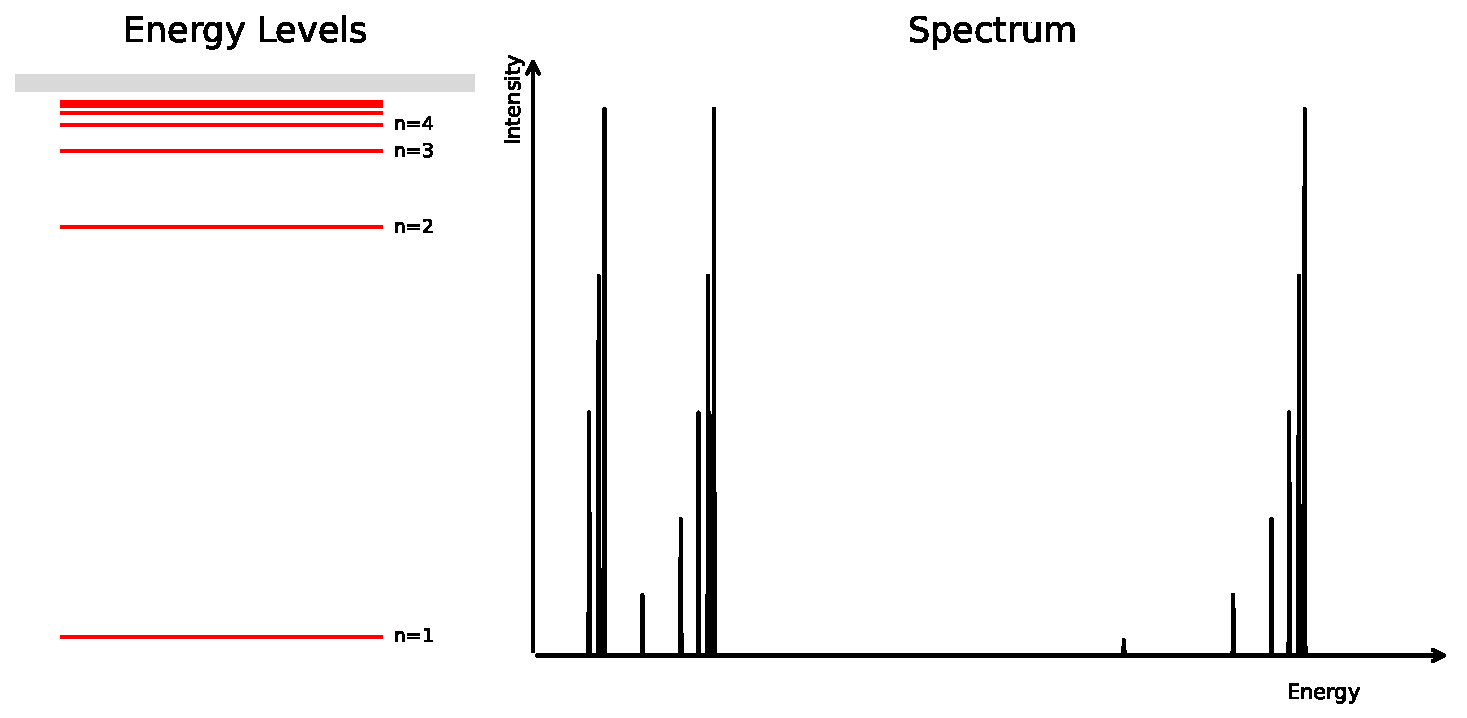
\includegraphics[width=.9\linewidth]{Figures/ElecSpectrum.pdf}
    \caption{The electronic energy levels and the corresponding spectrum, where the energy levels are populated according to the Boltzmann distribution. In the left panel, the energy levels corresponding to different principal numbers $n$ are shown. The energy levels get closer and closer together as the energy gets higher, until the ionization energy is marked with the gray bar. The right panel shows the spectral lines with the different groups of lines corresponding to Lyman, Balmer, and Paschen from right to left.}
    \label{fig: elec}
\end{figure}

In \autoref{fig: elec}, the collection of lines on the high-energy side corresponds with the Lyman series. The collection of lines to the left of it corresponds to the Balmer series, etc.
The electronic transitions typically occur in the ultraviolet (UV) and visible (VIS) parts of the electromagnetic spectrum, but higher order series, like Pfund and Hemphryes, can be found in IR. For example, the transition from $n=2$ to $n=1$, the Ly$\alpha$ transition, occurs at 121.567 nm.


\subsection{Vibrational Transition}
Vibrational transitions are corrections to the energy states set by the electronic transitions. This transition changes the vibration of the molecule. 
The bonds between atoms in a molecule can be viewed as springs connecting the atoms. These springs can have different motions, such as stretching and bending. The energies of these motions are discrete and given by: 

\begin{equation}
    E^{\mathrm{vib}}=\hbar\omega(v+1/2),
\end{equation}

where $\hbar$ is the reduced Planck constant $\left(\hbar=h/2\pi\right)$, $\omega=\sqrt{k/\mu}$ with $k$ the force constant and \textmu  reduced mass, and $v$ the vibrational quantum number. Transitions between energy states follow the selection rule: $\Delta v=\pm 1$. This means the only permitted transitions occur between energy levels with a vibrational quantum number that is one lower or higher than the current state. This results in the difference in energy between states to be

\begin{equation}
    \Delta E^{\mathrm{vib}}=\hbar\omega.
\end{equation}

The energy levels and the resulting spectrum are shown in \autoref{fig: vib}.

\begin{figure}[H]
    \centering
    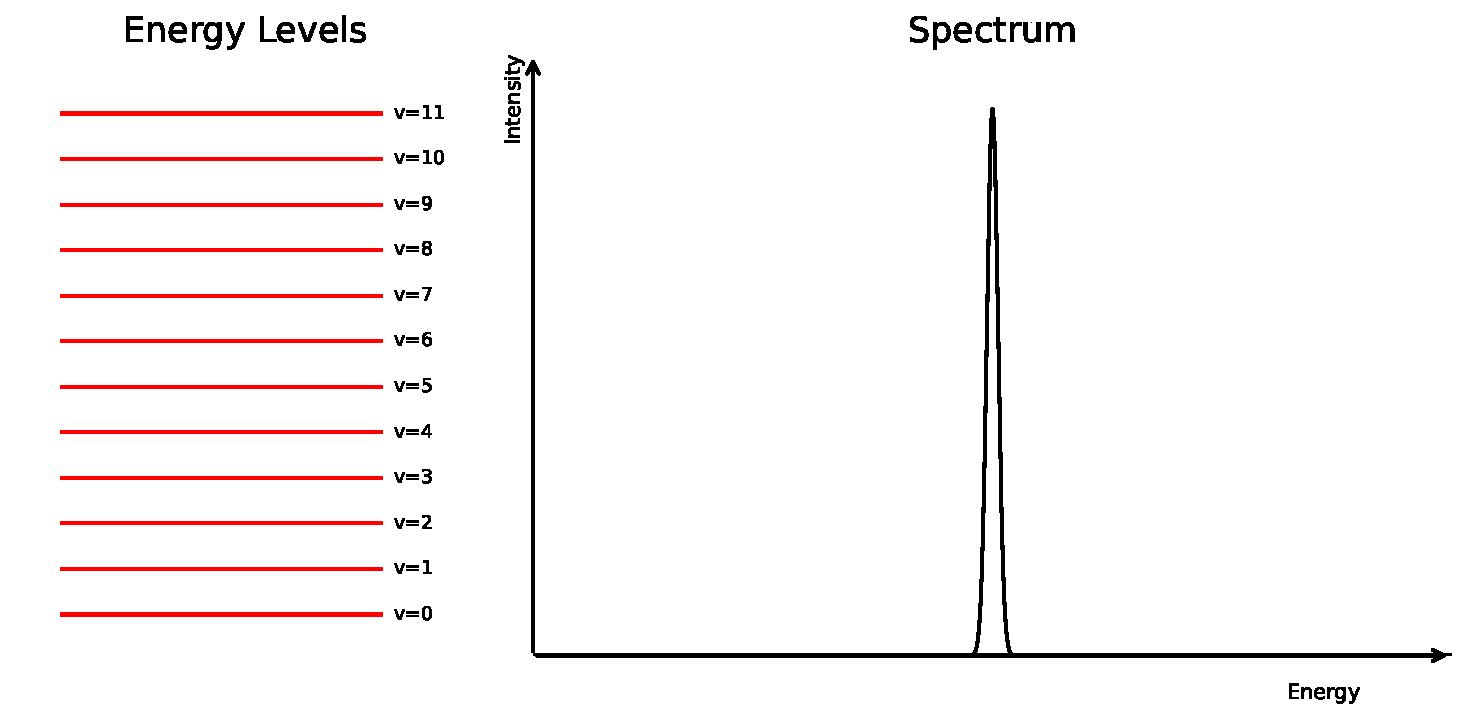
\includegraphics[width=0.9\linewidth]{Figures/VibSpectrum.pdf}
    \caption{The vibrational energy levels and the corresponding spectrum, where the energy levels are populated according to the Boltzmann distribution. The left panel shows the energy levels corresponding to the different vibrational quantum numbers $\nu$. The right panel show a single line as the energy transitions only occur between adjacent lines, and the energy difference between adjacent energy levels is the same.}
    \label{fig: vib}
\end{figure}

The vibrational transitions typically occur in the infrared (IR) part of the electromagnetic spectrum. 


\subsection{Rotational Transition}
The transition with the lowest energy is the rotational transition. This transition changes the angular momentum of the molecule. Molecules rotate with discrete energies given by:

\begin{equation}
    E^{\mathrm{rot}}=B_\mathrm{e}J(J+1)
\end{equation}

where $B_\mathrm{e}$ is the rotational constant, and $J$ is the rotational quantum number. 
The degeneracy of each state is $g(J)=2J+1$. Transitions between energy states follow the selection rule: $\Delta J=\pm 1$. This means the only permitted transitions occur between energy levels with a rotational quantum number that is one lower or higher than the current state. This results in the energy difference between a state with rotational quantum number $J+1$ to the state with rotational quantum number $J$ to be

\begin{equation}
    \Delta  E^{\mathrm{rot}}=2B_e(J+1).
\end{equation}

The energy levels and the resulting spectrum following the Boltzmann distribution are shown in \autoref{fig: ro}.

\begin{figure}[H]
    \centering
    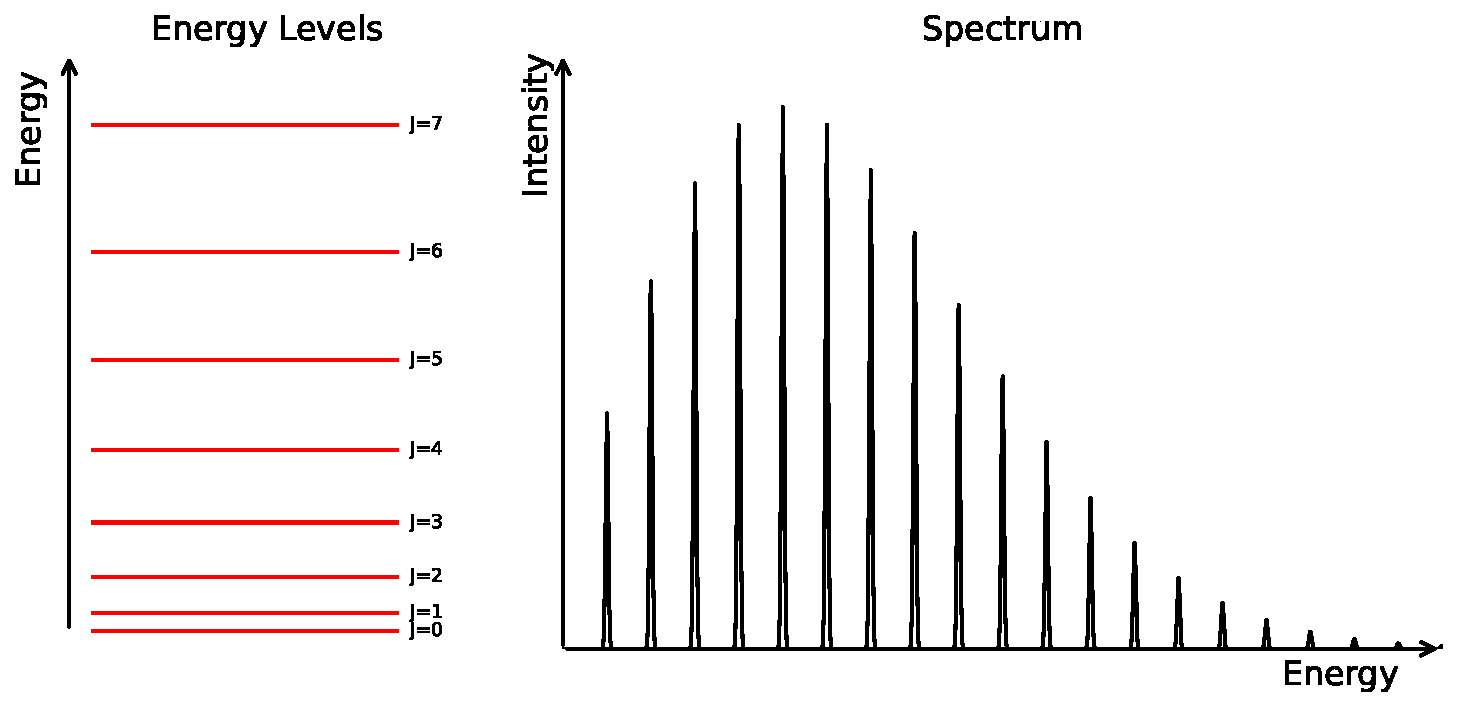
\includegraphics[width=0.9\linewidth]{Figures/RoSpectrum.pdf}
    \caption{The rotational energy levels and the corresponding spectrum, where the energy levels are populated according to the Boltzmann distribution. The left panel shows the energy levels corresponding to the different rotational quantum numbers $J$. The right panel shows the spectrum resulting from the energy levels.}
    \label{fig: ro}
\end{figure}

The rotational transitions typically occur in the microwave and radio parts of the electromagnetic spectrum.

\subsection{Ro-vibrational Transition}
In nature, pure vibrational transitions are rare. Often, the vibrational transitions are accompanied by rotational transitions. The combination of these two transitions is called a ro-vibrational transition. Transitions between energy states follow the selection rules: $\Delta v=\pm 1$, $\Delta J=0, \pm 1$. Plotting the energy levels and the resulting spectrum following the Boltzmann distribution gives \autoref{fig: rovib}.

\begin{figure}[H]
    \centering
    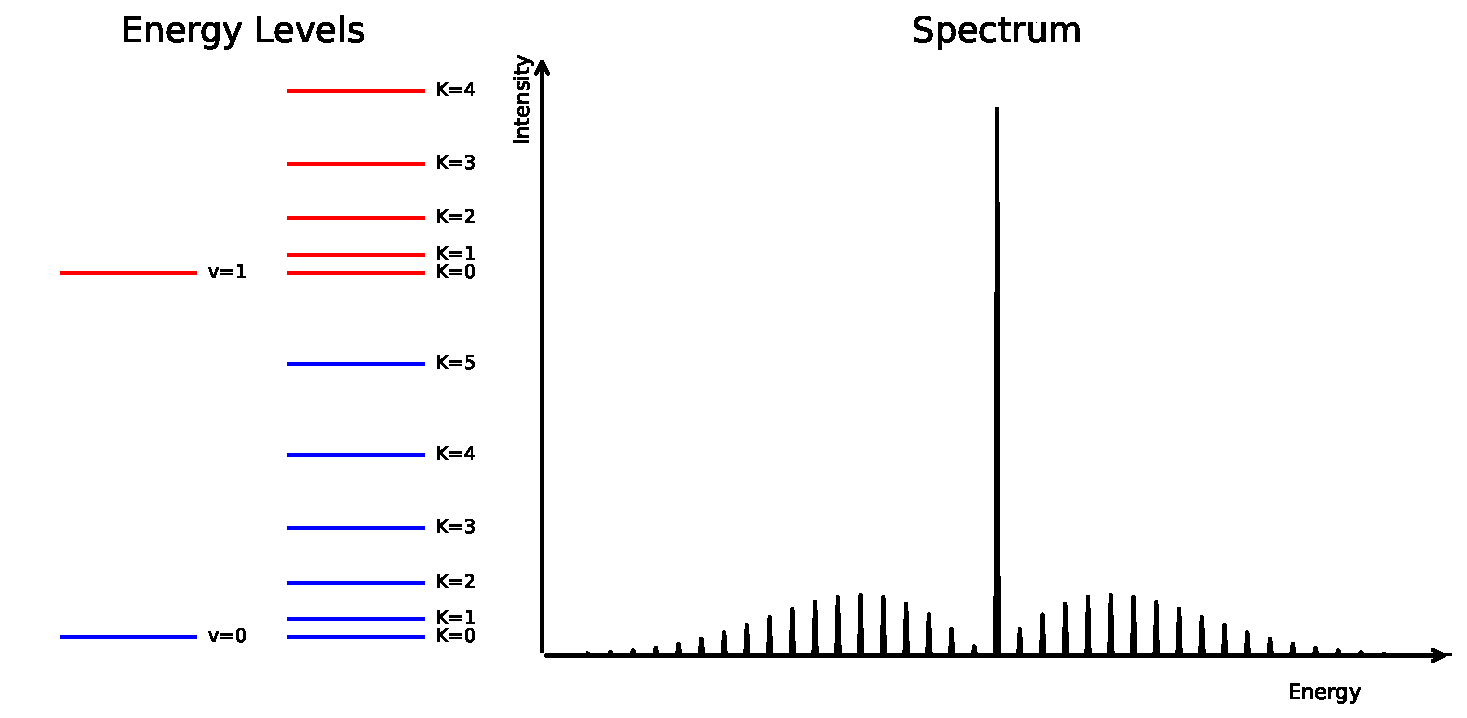
\includegraphics[width=0.9\linewidth]{Figures/RoVibSpectrum.pdf}
    \caption{The ro-vibrational energy levels and the corresponding spectrum, where the energy levels are populated according to the Boltzmann distribution. In the left panel, the different rotational energy states are added to the spectrum. The resulting spectrum is shown in the right panel. The P, Q, and R branches are highlighted in the spectrum. }
    \label{fig: rovib}
\end{figure}

In \autoref{fig: rovib}, a distinctive shape is visible: P, Q, and R branches. The P branch is the set of peaks with a lower energy than the central peak. The Q branch is the central peak, and the set of peaks on the higher energy side of the peak is the R branch. The P, Q, and R branches correspond to $\Delta J=1, 0, -1$ respectively. For some molecules and some vibrational modes, the transition with $\Delta J=0$ is forbidden. This also means that the Q branch is missing in the spectrum. This is, for example, the case for the ro-vibrational band of CO at $\sim$ 4 \textmu m.

\section{JWST MIRI MRS}
The James Webb Space Telescope (JWST) was launched on the 25th of December 2021. JWST was a big leap forward for space research. One of the instruments on board is the Mid-Infrared Instrument (MIRI). This instrument is used for observations in the mid-infrared. MIRI has four observation modes in the wavelength range between 4.9 and 27.9 \textmu m:  imaging, coronagraphic imaging, low-resolution spectroscopy, and medium-resolution spectroscopy (MRS) \citep{2023PASP..135d8003W}. This wavelength range overlaps with several spectral features of molecules, like H\2O and CO\2.
The wavelength region covered by MIRI MRS is of particular interest as it probes the inner regions of protoplanetary disks. In this case, MRS is preferred over LRS as the higher resolution allows for the detection of weaker features. MIRI MRS is an integral field spectrograph (IFS), which provides both spatial and spectral information. MIRI MRS uses four integral field units (IFU), each covering a different part of the spectrum. They are named channels 1 through 4. Additionally, MIRI MRS has three grating settings: short, medium, and long. It can take simultaneous exposures in the 4 channels using one of the grating settings. The channels have different fields of view (FOV) ranging from (3.2 $\times$ 3.7) arcsec to (6.6 $\times$ 7.7) arcsec. 

\begin{table}[H]
\centering
\begin{tabular}{lccc}
\toprule
\textbf{Spectral Band} &
\shortstack{\textbf{FOV} \\ \textbf{[arcsec]}} &
\shortstack{\textbf{Wavelength Range} \\ \textbf{[\textmu m]}} &
\textbf{Resolving Power} \\
\midrule
1short  & 3.2 $\times$ 3.7 & 4.9--5.74     & 3,320--3,710 \\
1medium & 3.2 $\times$ 3.7 & 5.66--6.63    & 3,190--3,750 \\
1long   & 3.2 $\times$ 3.7 & 6.53--7.65    & 3,100--3,610 \\
2short  & 4.0 $\times$ 4.8 & 7.51--8.77    & 2,990--3,110 \\
2medium & 4.0 $\times$ 4.8 & 8.67--10.13   & 2,750--3,170 \\
2long   & 4.0 $\times$ 4.8 & 10.02--11.70  & 2,860--3,300 \\
3short  & 5.2 $\times$ 6.2 & 11.55--13.47  & 2,530--2,880 \\
3medium & 5.2 $\times$ 6.2 & 13.34--15.57  & 1,790--2,640 \\
3long   & 5.2 $\times$ 6.2 & 15.41--17.98  & 1,980--2,790 \\
4short  & 6.6 $\times$ 7.7 & 17.70--20.55  & 1,460--1,930 \\
4medium & 6.6 $\times$ 7.7 & 20.69--24.48  & 1,680--1,770 \\
4long   & 6.6 $\times$ 7.7 & 24.19--27.9 & 1,630--1,330 \\
\bottomrule
\end{tabular}
\caption{MIRI MRS channel properties \citep{Argyriou_2023}. The first column is the spectral band where the number corresponds to the channel, and short, medium, and long to the grating setting. The second column shows the FOV of the different spectral bands. The third column displays the wavelength range in which the different spectral bands operate, and the resolving power is shown in the fourth column.}
\label{tab: MRS properties}
\end{table}

To reduce thermal noise, MIRI MRS operates at near-zero temperatures ($\sim$ 7 K), which is especially important for observations in IR \citep{2023PASP..135d8003W}. 
\textbf{Mention Spitzer}


\section{Modeling of Protoplanetary Disks}
Some of the properties of the protoplanetary disks can be directly inferred from disk measurements. For instances where this is not the case, we would still like to learn more from our data via a different method. Models can be used to simulate the protoplanetary disk and generate synthetic spectra for comparison with actual observations. In this way, the physical properties of the disk can be inferred.
When researching models, it is common to vary one or more parameters to see what effect it has on the output of the model. The set of these models with variations is often referred to as a model grid. The reference model, or fiducial model, is the model that commonly uses standard parameters and from which all other models in the grid were varied. The grid can be used to fit the data (e.g., Bayesian inference).

\subsection{Model Overview}
There are various types of models, ranging from local thermal equilibrium (LTE) slab models to thermo-chemical disk models. Below, we explain the models from simplest to most complex \citep{chap13}.
\begin{itemize}
    \item \textbf{LTE slab model} \\
    These models assume a single value for the volume density. The only parameters these models depend on are temperature and surface density. Additionally, local thermal equilibrium (LTE) is often assumed. Their simplicity allows for fast computation and works well for emissions coming from a small region in the disk, but it has limitations for deeper analysis.

    \item \textbf{1D slab model} \\
    In reality, the temperature and number density of molecules vary across protoplanetary disks. 1D slab models are an improvement on their LTE counterparts as they assume that the temperature and column density can be parametrized by a power law. These models have 2 more parameters, namely the power index of the column density and the power index of the temperature.

    \item \textbf{Dust disk structure model with parametrized chemistry} \\
    For these types of models, different molecules are combined into a single model, where the column density and temperature are described by a power law and can be different depending on the molecule. In the models, it is often assumed that the gas temperature and dust temperature are coupled, meaning they are the same. The dust temperature, and with it the gas temperature, are found using the disk structure. Ray tracing is used to simulate the spectra produced by the disk. The chemistry is parametrized by a simple function, such as a step function, where the abundance for a certain molecule is 0 when the temperature is below some threshold and a preset abundance above the threshold.

    \item \textbf{Dust disk structure model with parametrized chemistry\\ and parametrized hot gas layer} \\
    An improvement on the previous model is to allow the dust temperature and the gas temperature to decouple. This is not only what is observed in observations, but also important to detect spectral lines. These lines are only visible when the material that is creating the lines is hotter than the material creating the continuum; in other words, the temperature of the gas must be higher than the temperature of the dust for the lines to be visible.

    \item \textbf{Thermochemical disk model} \\
    The most complex models are thermochemical disk models. These calculate the dust temperature using radiative transfer, and find the gas temperature using heating and cooling mechanism and the chemistry in the disks. These models provide a full picture of the density of molecules throughout the disk and the temperature gradients. However, a downside of this accuracy is that it takes large amounts of computing power to run these simulations compared to simpler models, such as LTE models. 
\end{itemize}

\subsection{ProDiMo}
For our research, we utilize simulations using the Protoplanetary Disk Model (ProDiMo), a thermochemical disk model. ProDiMo is designed to produce realistic models of protoplanetary disks. ProDiMo models both the gas and dust in a disk using a 2D slice of the disk and assumes that the disk is axisymmetric.

\begin{figure}[H]
    \centering
    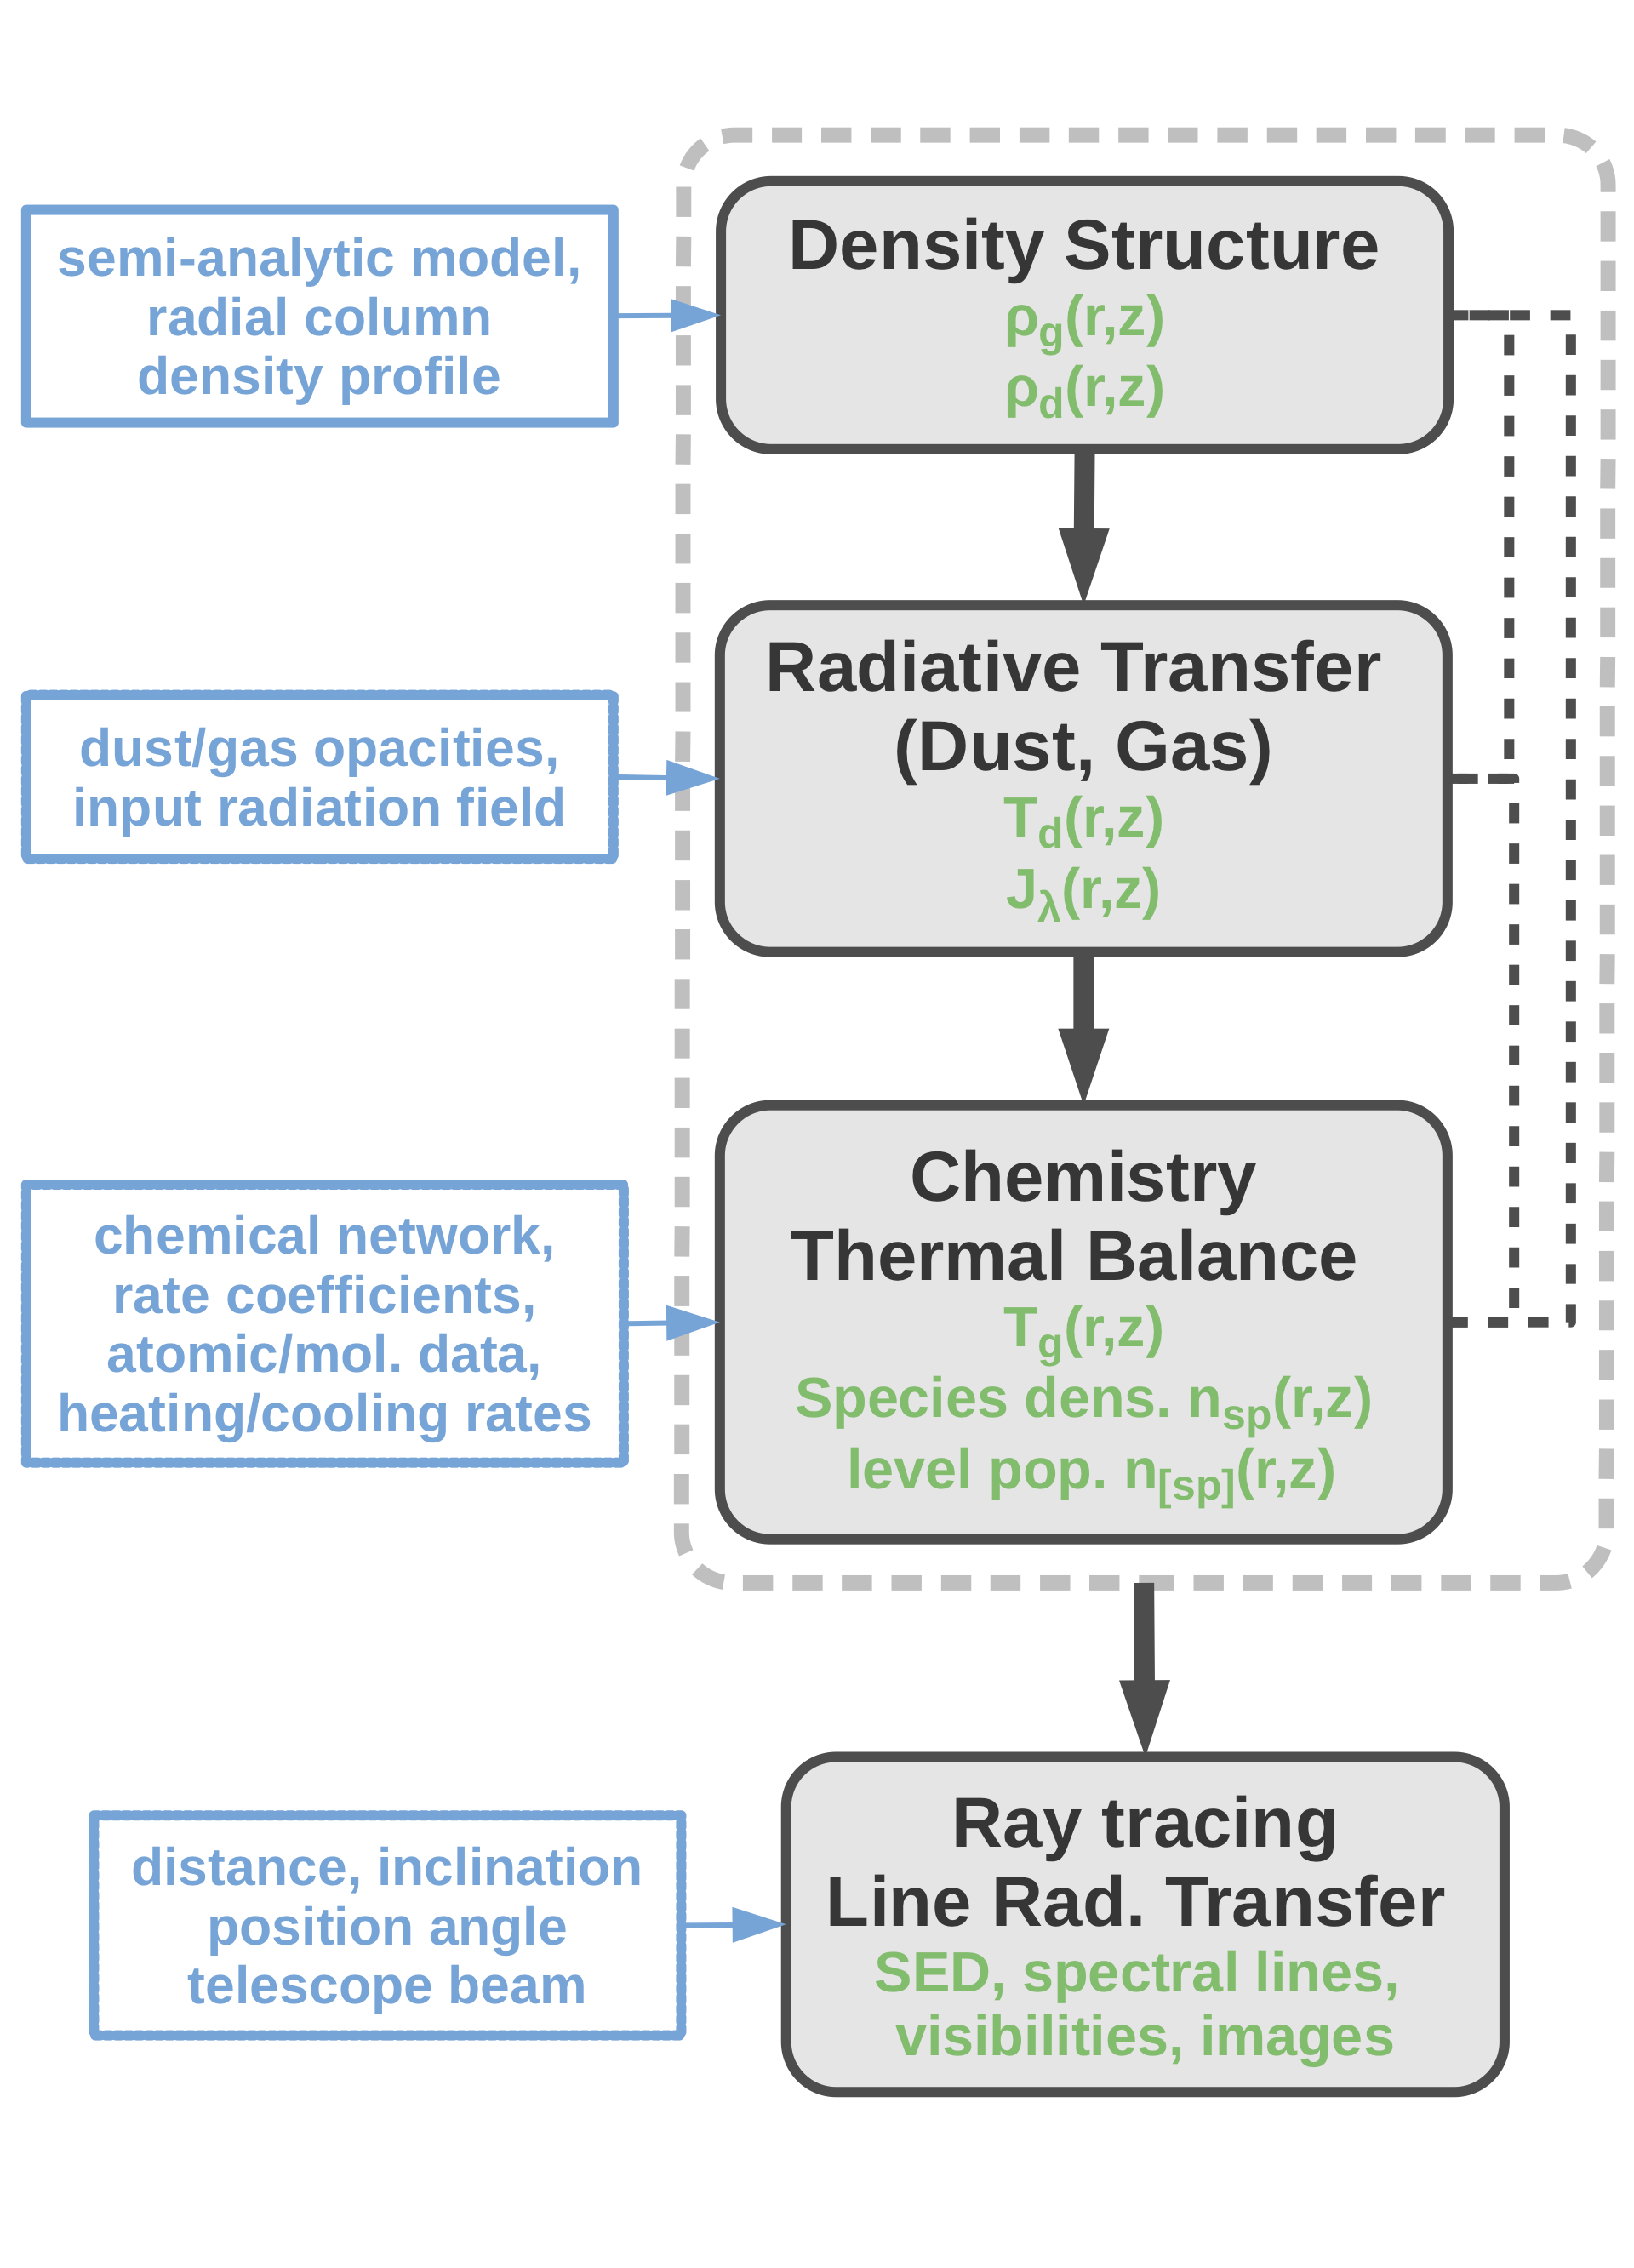
\includegraphics[width=0.5\linewidth]{Figures/prodimoflowchart (1).png}
    \caption{The flowchart of the ProDiMo code. Source: \href{https://prodimo.iwf.oeaw.ac.at/}{ProDiMo Official Website}$^*$}
    \label{fig:enter-label}
\end{figure}
\footnotetext{$^*$\href{https://prodimo.iwf.oeaw.ac.at/}{https://prodimo.iwf.oeaw.ac.at/}}
To start a simulation, several parameters need to be set. Firstly, the gas and dust densities for different radii and heights above the midplane must be defined. Moreover, stellar parameters, like stellar mass, effective temperature, stellar luminosity, UV, and X-ray, are set. Similarly, interstellar properties need to be defined, like the IR background, the UV background, and cosmic rays (CR). 

After setting all the parameters, ProDiMo starts the simulation. It performs the radiative transfer, which yields the dust temperature and the radiation field at every point in the disk. This is followed by a chemical thermal balance, which provides the gas temperature, the density of different molecules, and the excitation levels of the molecules. 

The gas density can be found using
\begin{equation}
    \rho_\mathrm{g}(r,z)=\frac{\Sigma(r)}{\sqrt{2\pi}h(r)}\exp{\left(-\frac{z^2}{2h(r)^2}\right)},
    \label{eq: density}
\end{equation}
where $\Sigma(r)$ is the surface density, $h(r)$ the scale height (which can be calculated using hydrostatic equilibrium. 

There are several methods to calculate the dust density: fixed gas-to-dust mass ratio, radius-dependent gas-to-dust mass ratio, grain size-dependent gas-to-dust mass ratio, and settling. 

To find the radiation field, \autoref{eq: radiative transfer} is used.
\begin{equation}
    \frac{1}{\rho(\vec{r})}\frac{\partial I_\nu(\rho(\vec{r}, \hat{k}))}{\partial s}=-\kappa^{\mathrm{ext}}_\nu I_\nu(\rho(\vec{r}, \hat{k})) + \kappa^{\mathrm{abs}}_\nu B_\nu(T(\vec{r})) + \kappa^{\mathrm{sca}}_\nu J_\nu(\vec{r})
    \label{eq: radiative transfer}
\end{equation}
where 

It is further assumed that the disk is in radiative equilibrium 
\begin{equation}
    \int^\infty_0\kappa^{\mathrm{abs}}_\nu B_\nu(T(\vec{r}))d\nu=\int^\infty_0\kappa^{\mathrm{abs}}_\nu J_\nu(\vec{r})d\nu
\end{equation}

which gives the dust temperature. 

\textbf{chemistry}
This is iteratively repeated until the dust temperature converges.
\subsection{FLiTs}
The output of ProDiMo models can be processed through the Fast Line Tracing system (FLiTs) to get an accurate spectrum of the disk. \cite{Woitke_2018} describes the development of FLiTs. FLiTs was developed as a tool to overcome some challenges that simulating spectra in the IR poses. This spectral region contains a great number of emission lines and energy levels. Disks are complex; light can be emitted in one region of the disk and reabsorbed elsewhere. Lastly, the full radiative transfer equation must be solved, as high optical depths are involved. At the time of the development of FLiTs, there was another code available named RadLite \citep{Pontoppidan_2009}. However, this code was slow and 
calculated the spectrum on a line-to-line basis, which prevented it from accurately describing line blending. So a new code, FLiTs, was developed to tackle these problems. 

All quantities, such as density and temperature, are provided to FLiTs from ProDiMo and transformed from a points-based grid to a cell-based grid. The model assumes Keplerian rotation and ignores the small effects from the pressure gradient, which can slow down the rotation of the disk by a few percent. Parallel rays are then cast through the disk at the inclination angle. The solution of the radiative transfer equation per wavelength is then integrated along these rays to produce the spectrum. To avoid aliasing, it uses randomized spatial and spectral sampling. As each part of the disk contributes to different parts of the spectrum, bundles of rays are used at random locations. The accuracy is determined by the number of rays, which means higher spatial resolution.




\chapter{Methods}\label{Ch: Methods}
In this chapter, we explain the methodology used in our work. Firstly, we go over the simulations that we used and how they were analyzed. Thereafter, we explain the cross-correlation technique and how this can be used to detect the emission of molecules in spectra. Lastly, we explain the observations and how the upper limits on the column densities of NO and NH\3 are determined.

\section{ProDiMo Simulations}
We used a grid of ProDiMo models with varying abundances of C and O, to investigate whether we can detect NO and NH\3 in the spectra of protoplanetary disks and how nitrogen carriers depend on the C and O abundance. The parameters with which the models were run are given in \autoref{tab: parameters}.

\begin{equation}
    \epsilon_X\equiv\log\frac{N_X}{N_H}+12
\label{eq: abundance}
\end{equation}

The abundances in the models are defined as in \autoref{eq: abundance}, where the abundance of some element X ($\epsilon_X$) depends on the based-10 logarithm (denoted as $\log$) of the ratio of the number density of that element ($N_X$) to the number density of hydrogen ($N_H$). In this system, $\epsilon_H=12$ by definition. The difference in abundances of C and O compared to solar abundances was varied between -0.5 and 0.5 in steps of 0.25, where a difference of 0 corresponds to the solar abundance. The grid contains 25 models, with the fiducial model in the middle, which is based on the solar abundances of C and O (see \autoref{tab: abundances}).

Additionally, the nitrogen abundance was increased by one order of magnitude compared to the solar abundance to investigate the effects on the spectrum and to enhance the spectral features of nitrogen carriers, thereby making their detection easier.

\begin{table}[H]
\centering
\begin{tabular}{@{}lll@{}}
                                  &                             &                            \\ \hline\midrule
\textbf{Property}                 & \textbf{Symbol}             & \textbf{Value}             \\ \midrule
Stellar mass                      & M$_\ast$                    & 0.7 M$_\odot$               \\
Effective Temperature             & T$_\ast$                    & 4000 K                     \\
Stellar Luminosity                & L$_\ast$                    & 1 L$_\odot$                \\
UV excess                         & f$_{\mathrm{UV}}$                    & 0.01                       \\
UV powerlaw index                 & p$_{\mathrm{UV}}$                    & 1.3                        \\
X-ray luminosity                  & L$_\mathrm{X}$                       & 10$^{30}$ erg s$^{-1}$              \\
X-ray emission temperature        & T$_\mathrm{X}$                       & 2$\times10^7$ K            \\ \midrule
Strength of interstellar UV       & $\chi^{\mathrm{ISM}}$                & 1                          \\
Strength of interstellar IR       & $\chi^{\mathrm{ISM}}_{\mathrm{IR}}$           & 0                          \\
Cosmic ray H$_2$ ionization rate  & $\zeta_{\mathrm{CR}}$                & $1.7\times10^{-17}$ s$ ^{-1}$ \\ \midrule
Inner disk radius                 & R$_{\mathrm{in}}$                    & 0.05 au                    \\
Outer disk radius                 & R$_{\mathrm{tap}}$                   & 30 au                      \\
Column density power index        & $\epsilon$                  & 1                          \\
Reference scale height            & H$_g$ (100 au)              & 10 au                      \\
Flaring power index               & $\beta$                     & 1.15                       \\ \midrule
Minimum dust particle radius      & a$_{\mathrm{min}}$                   & 0.05 \textmu m                \\
Maximum dust particle radius      & a$_{\mathrm{max}}$                   & 3000 \textmu m                \\
Dust size dist. power index       & a$_{\mathrm{pow}}$                   & 3.5                        \\
Turbulent mixing parameter        & $\alpha_{\mathrm{settle}}$           & 0.001                      \\
Refractory dust composition       & Mg$_{0.7}$Fe$_{0.3}$SiO\3 & 60 \%                      \\
                                  & amorph. C                   & 15 \%                      \\
                                  & porosity                    & 25 \%                      \\
PAH abundance rel. to ISM         & f$_{\mathrm{PAH}}$                   & 0.01                       \\
Chemical heating efficiency       & $\gamma^{\mathrm{chem}}$             & 0.2                        \\ \midrule
Distance to the observer          & d                           & 140 pc                     \\ \bottomrule
\end{tabular}
\caption{Disk parameters used for the grid of ProDiMo models}
\label{tab: parameters}
\end{table}


The output of the ProDiMo model grid was used to generate the mid-infrared spectra using FLiTs. The full spectrum includes emission from C\2H\2, CH\4, CO, CO\2, H\2O, HCN, NH\3, NO, OH. In addition, FLiTs produced spectra containing the emissions of the individual molecules. The FLiTs spectra were calculated at a very high spectral resolution ($R=10^5$). To make the spectra more comparable to the JWST MIRI MRS spectra, the spectra were convolved to a resolving power of $R = \lambda/\Delta\lambda = 3000$ using a Gaussian kernel to create spectra of the same resolving power. The value of 3000 was chosen as it is approximately the average resolving power of the JWST MIRI MRS \citep{Argyriou_2023}. 

\begin{table}[H]
\centering
\begin{tabular}{@{}ccc@{}}
                                  &                             &                            \\ \hline\midrule
\textbf{Element} & \textbf{+12 Abundance} & \textbf{Variation}            \\ \midrule
H                & 12                     & Fixed                         \\
He               & 10.98                 & Fixed                         \\
C                & 8.14                  & {[}-0.5, -0.25, 0, +0.25, +0.5{]} \\
N                & 8.90                  & Fixed                         \\
O                & 8.48                  & {[}-0.5, -0.25, 0, +0.25, +0.5{]} \\
Ne               & 7.95                  & Fixed                         \\
Na               & 3.36                  & Fixed                         \\
Mg               & 4.03                  & Fixed                         \\
Si               & 4.24                  & Fixed                         \\
S                & 5.27                  & Fixed                         \\
Ar               & 6.08                  & Fixed                         \\
Fe               & 3.24                  & Fixed                         \\
PAH              & 3.44                  & Fixed                         \\ \bottomrule
\end{tabular}
\caption{The elemental abundances used in the simulation of the grid of ProDiMo models. The solar abundances were used, except for N, which was enhanced by one order of magnitude.}
\label{tab: abundances}
\end{table}

\subsection{Noise Addition}
Noise was added to the simulated spectra to make them more realistic. The observations obtained by the MINDS JWST GTO program have a signal-to-noise ratio (SNR) of 300 on the continuum \citep{henning2024mindsjwstmirimidinfrared}. To make the simulated data align with an SNR = 300, the minimum of the simulated spectrum before continuum subtraction was used to find the variance $\sigma^2$ by using 

\begin{equation}
    SNR = \frac{F_{min}}{\sigma}\Rightarrow\sigma=\frac{F_{min}}{SNR}.
    \label{eq: SNR}
\end{equation}

The variance $\sigma^2$ was then used to add Gaussian noise to each flux value following 

\begin{equation}
    \tilde{F}_i = F_i + \varepsilon_i,\;\varepsilon_i\sim\mathcal{N}(0, \sigma^2).
    \label{eq: noise}
\end{equation}

After applying this noise, we subtracted the continuum. This continuum-subtracted spectrum was subsequently used for analysis.

\subsection{Flux Calculation}
The flux densities provided by FLiTs are in units of Jansky. To obtain the flux, we integrated the flux density by first converting the flux density from per unit frequency to per unit wavelength using

\begin{equation}
    F_\lambda=\frac{c}{\lambda^2}F_\nu,
    \label{eq: conversion}
\end{equation}

where $F_\lambda$ is the flux density in units of wavelength, $\lambda$ the wavelength, and $F_\nu$ the flux density in unit of frequency.
\subsection{Spectrum Classification}
Different species emit light in distinct spectral regions. To classify these regions, the entire spectrum was split into windows of 0.01 \textmu m from 4.9 to 27.5 \textmu m. The window size of 0.01 \textmu m was chosen, as it is approximately the expected window size at this spectral resolution ($R=\lambda/\Delta\lambda\Rightarrow\Delta\lambda=\lambda/R\approx30 $ \textmu$\mathrm{m}/3000=0.01$ \textmu$\mathrm{m}$). Next, we integrate the emission for each species in that window and note the species that has the highest flux in that region. Doing this for all models and taking the mode gives the species for each window that has the strongest emission for most of the simulated spectra.  

\newpage
\section{Cross-Correlation Technique}
For our analysis, we used cross-correlation. This is a signal detection technique used to detect weak signals. This technique was implemented to detect the weak spectral features of NO and NH\3. Cross-correlation is defined as follows 

\begin{equation}
    R_{fg}(\tau)=\int^\infty_{-\infty}\overline{f(t)}g(t+\tau)dt,
\end{equation}

where $R_{fg}(\tau)$ is the cross-correlation, $f$ and $g$ are functions of $t$, and $\tau$ is the lag. As all our functions are real valued, we can omit the complex conjugation in the integrand.

\begin{figure}[H]
    \centering
    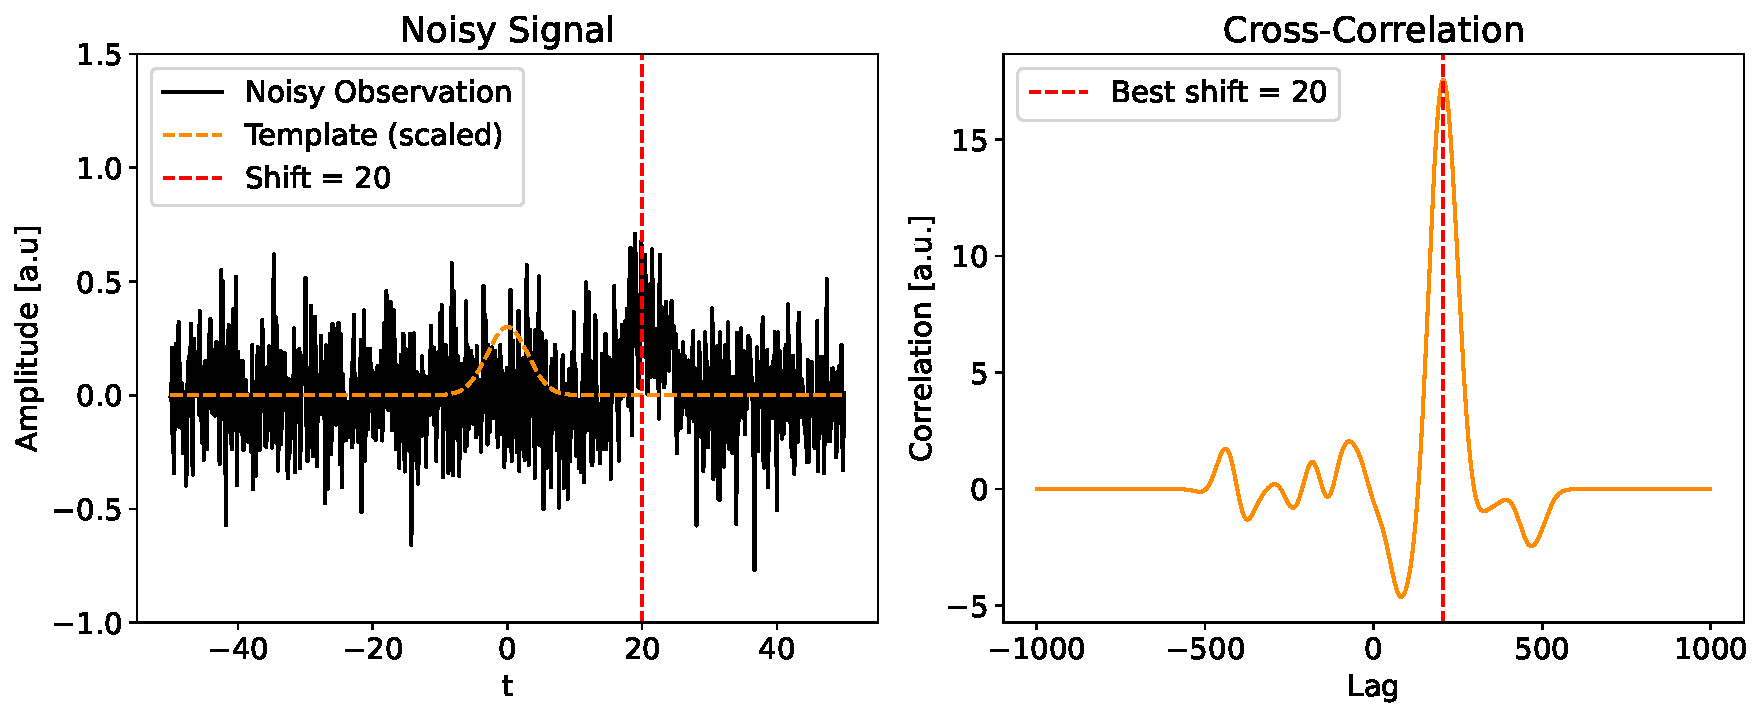
\includegraphics[width=\linewidth]{Figures/Correlationexample.pdf}
    \caption{The left plot shows a noisy signal that contains a Gaussian feature that is shifted to $t=20$. The right plot shows the cross-correlation of the Gaussian template signal with the noisy signal.}
    \label{fig: crosscorr vis}
\end{figure}

\autoref{fig: crosscorr vis} illustrates how the cross correlation can be used to detect a weak signal, and if it is detected, the location in the signal. On the left, the added Gaussian is barely visible, whereas on the right, there is a clear peak, which signals that the weak signal is present in the noise and its location.

\newpage
\subsection{Hypothesis Testing}
We used the emissions for each species across the model grid to apply this technique to spectra to test for the presence of specific molecules. For each molecule, the emission for each model was added together and normalized by dividing by the maximum, producing a template. This template emission was cross-correlated with the spectrum containing emission from all the species. The cross-correlation should peak when the template spectrum matches the spectrum containing all the species. To quantify the height of the peak, we calculated the difference between the height of the peak and the median value of the cross-correlation in a small region around the peak. The median, which was selected in favor of the mean as the median is less susceptible to outliers, captures the general trend around the peak. Hypothesis testing was implemented to test whether or not there is statistical evidence to say the molecule is present in the spectrum. We had the following null hypothesis and alternative hypothesis, with the difference between the height of the peak and the median of neighboring points as the test statistic.

\[
\begin{aligned}
H_0: &\ \text{The null hypothesis is that the height of the peak in the cross-} \\
     &\ \text{correlation is caused by the emission of noise;}\\
     \\
H_1: &\ \text{The alternative hypothesis is that the height of the peak in the} \\
     &\ \text{cross-correlation is caused by the emission of the molecule.}
\end{aligned}
\]

To assess the significance of the peak in cross-correlation, a Monte Carlo simulation was used to simulate 10000 synthetic spectra under the null hypothesis. First, all the flux values for different wavelength values are collected in a set. Second, flux values were sampled with replacement from the set until a collection of values was obtained that was the same size as the original set. This procedure is comparable to bootstrap sampling. In this way, a completely randomized spectrum is created, which simulates pure noise. Third, we calculated the cross-correlation of the randomized spectrum with the template and determined the difference between the peak height and the median value of the cross-correlation in a small region around the peak. Repeating these steps to create 10000 spectra, and with it corresponding values for the test statistic, resulted in a distribution. The peak is deemed significant, and thus the molecule is present, when its test statistic exceeds 95\% of the test statistic values from the randomized spectra ($\alpha=0.05$).

\newpage
\section{Observations}
After investigating the simulated spectra, the techniques were extended to observations made with JWST MIRI MRS. We have access to three sources: GWLup \citep{Gasman_2023}, Sz98 \citep{Grant_2023}, and V1094Sco \citep{taboneinprepp}. The spectra were already continuum-subtracted and are shown in \autoref{fig: Measurements}. However, the continuum subtraction left artifacts in the spectrum. The artefacts are non-physical features in the spectrum, such as peaks in the spectrum. \cite{Grant_2023} has listed the regions in the spectrum containing such artifacts, and that list of regions was used to mask out the artefacts. 

\begin{figure}[H]
    \centering
    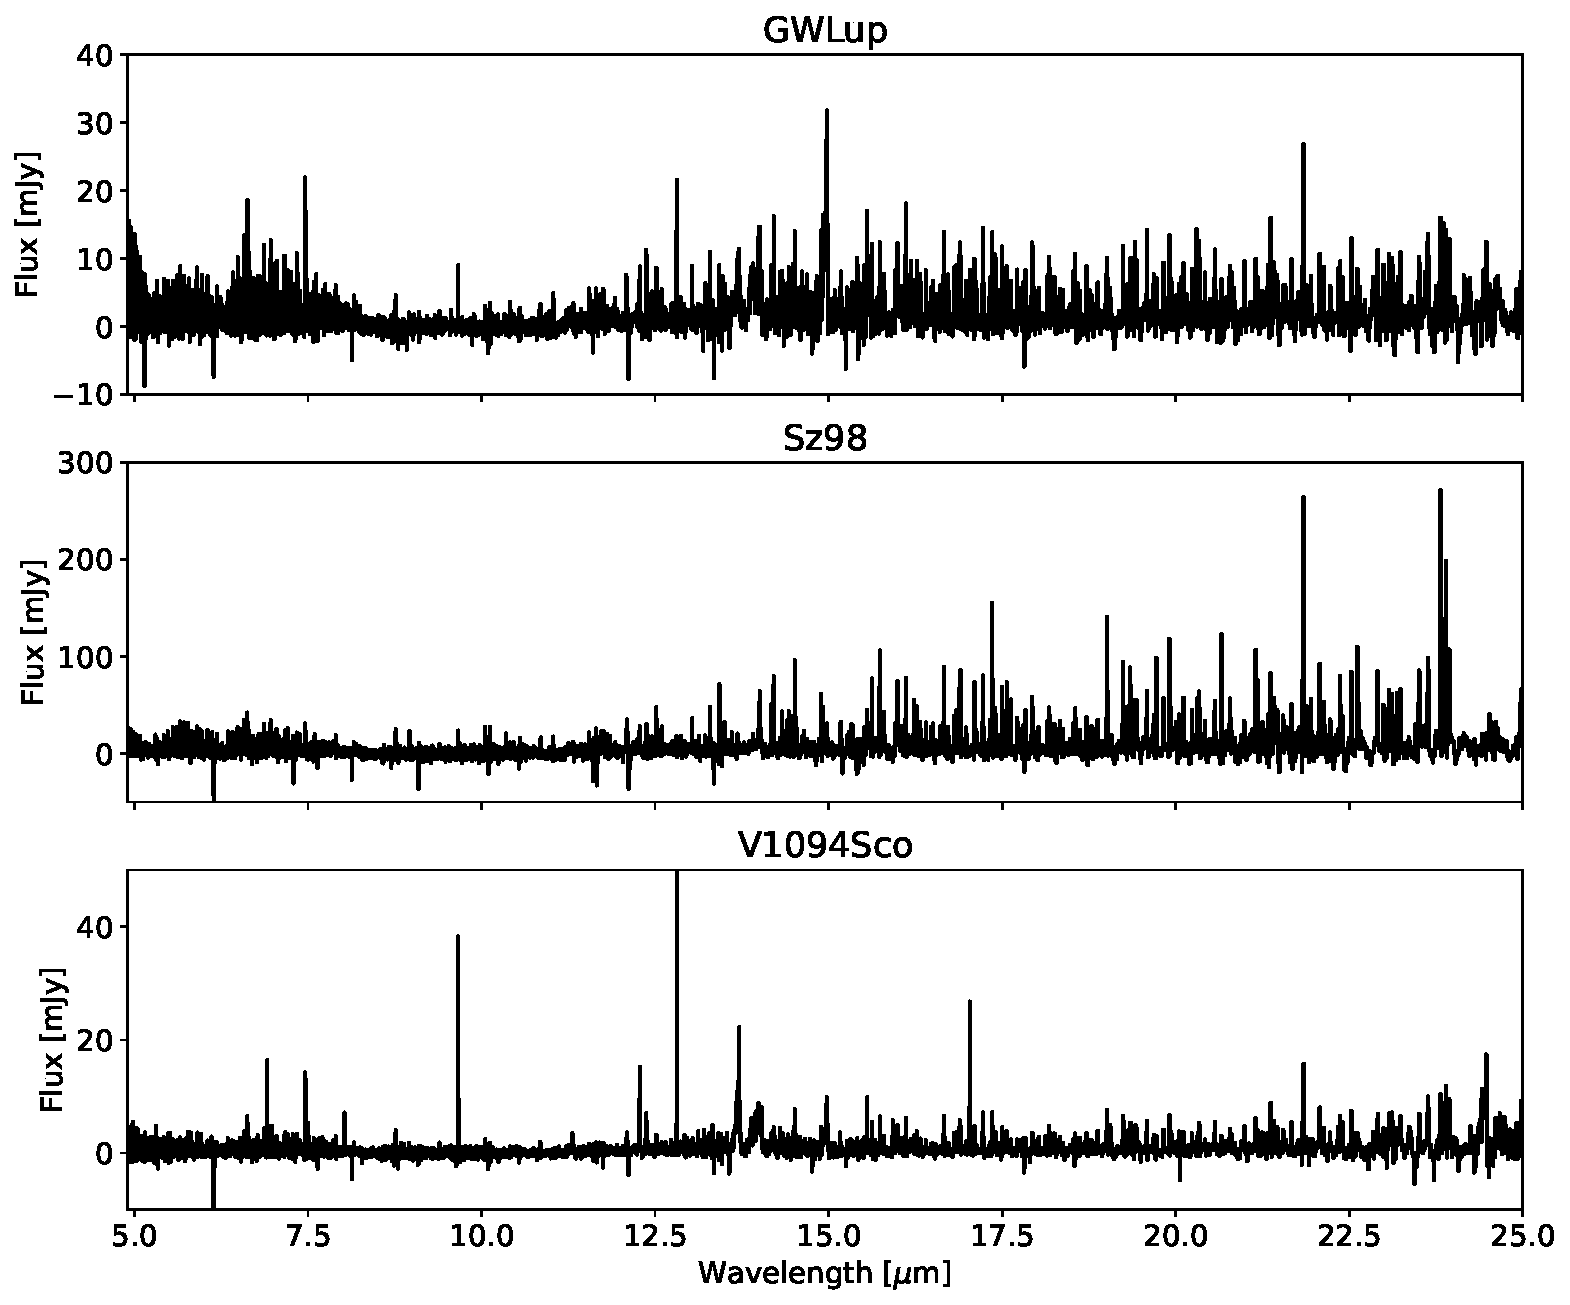
\includegraphics[width=\linewidth]{Figures/Measurements.pdf}
    \caption{The continuum subtracted JWST MIRI MRS spectra of GWLup \citep{Gasman_2023}, Sz98 \citep{Grant_2023}, and V1094Sco \citep{taboneinprepp}. Some of the notable spectral features are labeled using insets.}
    \label{fig: Measurements}
\end{figure}

\subsection{LTE Model Fitting}
LTE models were used to fit the observed spectra. A similar procedure to the process described by \cite{Grant_2023} was followed. This is based on least-squares fitting, which minimizes $\chi^2$ given by:

\begin{equation}
    \chi^2=\frac{1}{N}\sum_{i=1}^N\frac{(F_{i,\mathrm{obs}}-F_{i, \mathrm{mod}})^2}{\sigma^2}
    \label{eq: chi-square}
\end{equation}

where $N$ is the number of spectral elements, $F_{i,\mathrm{obs}}$ is the observed flux, $F_{i,\mathrm{mod}}$ is the modeled flux and $\sigma^2$ the variance in an emission-free region of the spectrum, the degrees of freedom (DOF) of the fit are two: column-density $N$ and temperature $T$. To retrieve an accurate spectrum, the distance and radial velocity (\autoref{tab: dist+rv}) must be taken into account. Larger distances result in smaller angular sizes, and the radial velocity causes the light to Doppler shift. The LTE model spectrum needs to be multiplied by the emitting area, which is assumed to be a disk with radius $R_e$. However, as this is just a scaling factor, $R$ is not considered a degree of freedom (DOF). The confidence intervals corresponding to 1$\sigma$, 2$\sigma$, and 3$\sigma$ are given by $\chi^2_{\mathrm{min}}+2.3$, $\chi^2_{\mathrm{min}}+6.2$, and $\chi^2_{\mathrm{min}}+11.8$ respectively \citep{pressetal, Avnietal}. The emission of the molecules was fitted iteratively. First, the emission per molecule was fitted to the spectrum. Second, the fits were improved by subtracting the fitted emission of all other molecules using the fitted spectra from the first step, except for the one that was being fitted, and fitting to the residuals. Lastly, the previous step is repeated one more time. 
The fitted spectra were used to find the emission of specific molecules and subtract them from the spectrum. This was used to find weaker emissions of NO and NH\3 in the residuals. 

\begin{table}[H]
\centering
\begin{tabular}{ccc}
\hline
Source   & \makecell{Distance \\\citep{henning2024mindsjwstmirimidinfrared}}  & \makecell{Radial velocity \\ \citep{Frasca_2017}} \\ \hline
GWLup    & 155.20 pc & -3.3 km/s       \\
Sz98     & 156.27 pc & -1.4 km/s       \\
V1094Sco & 152.44 pc & 2.2 km/s        \\ \hline
\end{tabular}
\caption{The distances and radial velocities of GWLup, Sz98, and V1094Sco}
\label{tab: dist+rv}
\end{table}

\newpage
\subsection{Determination of Upper Limits}
To produce an estimate on the upper limit, we used Bayes' theorem (\autoref{eq: Bayes}) to find the posterior distribution of the parameters. 

\begin{equation}
    P(\mathrm{model}|\mathrm{data})\propto P(\mathrm{data}|\mathrm{model})P(\mathrm{model})
    \label{eq: Bayes}
\end{equation}

where $P(\mathrm{model}|\mathrm{data})$ is the posterior distribution, $P(\mathrm{data}|\mathrm{model})$ the likelihood, and $P(\mathrm{model})$ the prior. Assuming that the residuals are normally distributed gives the likelihood

\begin{equation}
    P(\mathrm{data}|\mathrm{model})\propto\exp\left(-\frac{\chi^2}{2}\right),
\end{equation}

where $\chi^2$ is defined as in \autoref{eq: chi-square}. The ProDiMo models were used to set a lower limit $T_0$ on the temperature, which is implemented in the flat prior:

\begin{equation}
    P(\mathrm{model}) = 
    \begin{cases}
        1, & \text{if } T > T_0 \\
        0, & \text{if } T \leq T_0
    \end{cases}
\end{equation}

We combined the likelihood and prior using \autoref{eq: Bayes} to get the posterior distribution. Next, samples were drawn from this distribution. The upper limit on the column density was derived from the samples as the value below which 95\% of the samples fall. 


\chapter{Results}\label{Ch: Results}
This chapter explains our results. Firstly, we analyze the output of the ProDiMo models. Next, the FLiTs spectra and smaller spectral regions within are inspected. Thereafter, the cross-correlation technique is applied to the spectra. Lastly, we use the obtained knowledge to investigate observations and determine upper limits on the column densities of NO and NH\3.

\section{ProDiMo Output}\label{sec: Prodimo output}
% \textbf{COMPARING NON-ENHANCED TO ENHANCED}
After running the models, we analyzed their output. First, we looked at the densities of the gas and dust in the disk. The densities of the fiducial model are shown in the top row of \autoref{fig: tempdensity}. The density of the gas is more vertically extended than the density of the dust. This is expected, as the dust settles around the midplane. Furthermore, the gas density stretches farther from the host star than the dust.

\begin{figure}[H]
    \centering
    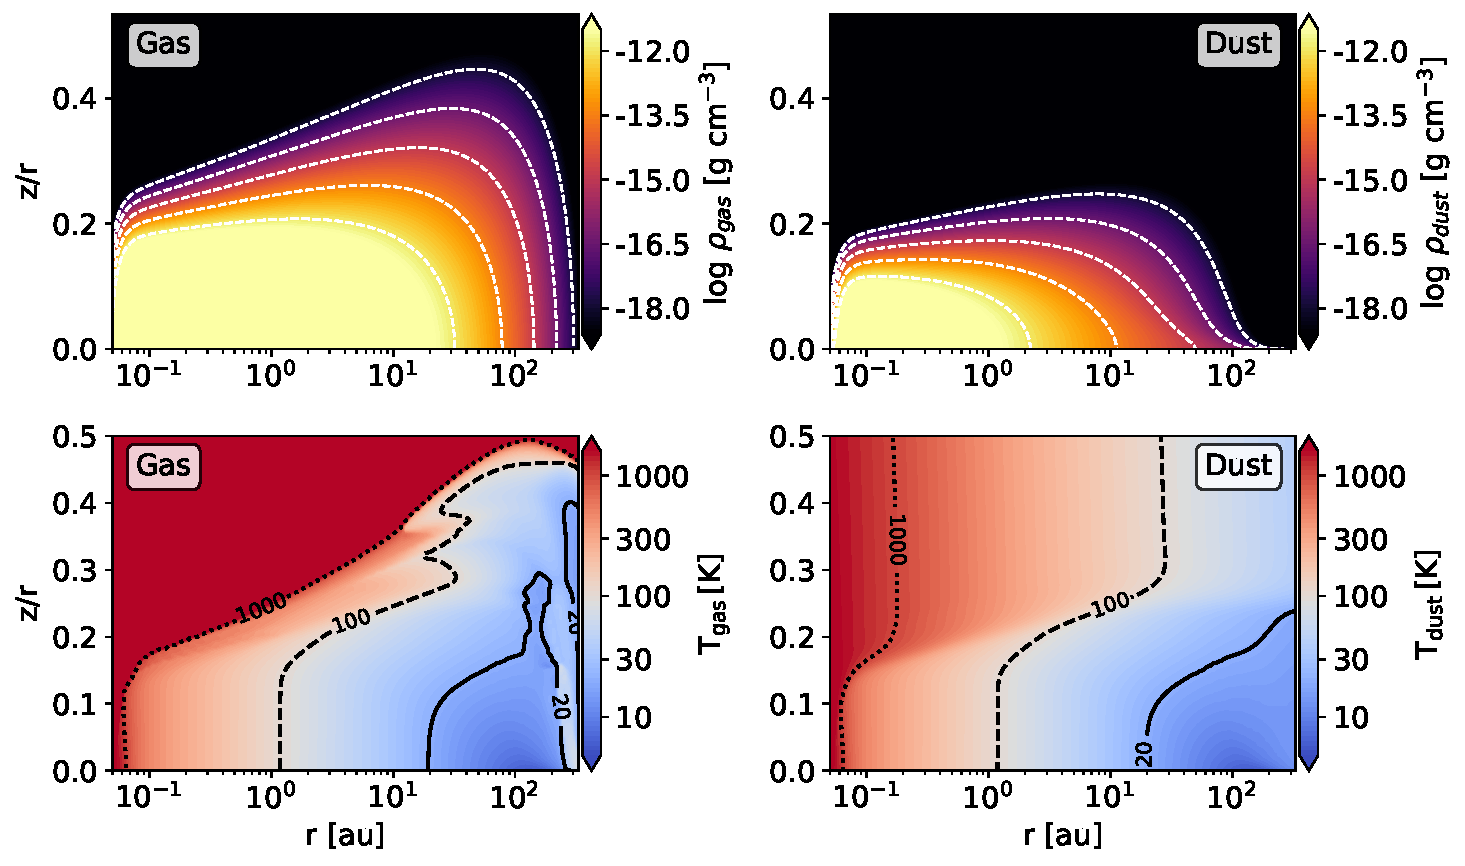
\includegraphics[width=\linewidth]{Figures/DensityTemperature.pdf}
    \caption{The density and temperature maps of gas and dust in the disk of the fiducial model. The horizontal axis shows the distance $r$ from the host star, and the vertical axis shows the height above the midplane $z$ divided by the radius $r$.}
    \label{fig: tempdensity}
\end{figure}

Next, we inspected the temperatures of gas and dust across the disk. Those are shown in the bottom row of \autoref{fig: tempdensity}.  The gas and dust temperatures vary across the disk for different heights and radii. However, they are equal in the midplane as they are coupled. Above the midplane, they decouple, and the temperatures of the gas and dust change. The gas temperatures are higher as they get heated by the star. Notably, the temperature of the dust is vertically isothermal. This result is expected as the density of the dust is orders of magnitude lower than that of the gas in the upper regions of the disk.  As a result, starlight passes through with minimal obstruction, leading to little variation in temperature with height.


\begin{figure}[H]
    \centering
    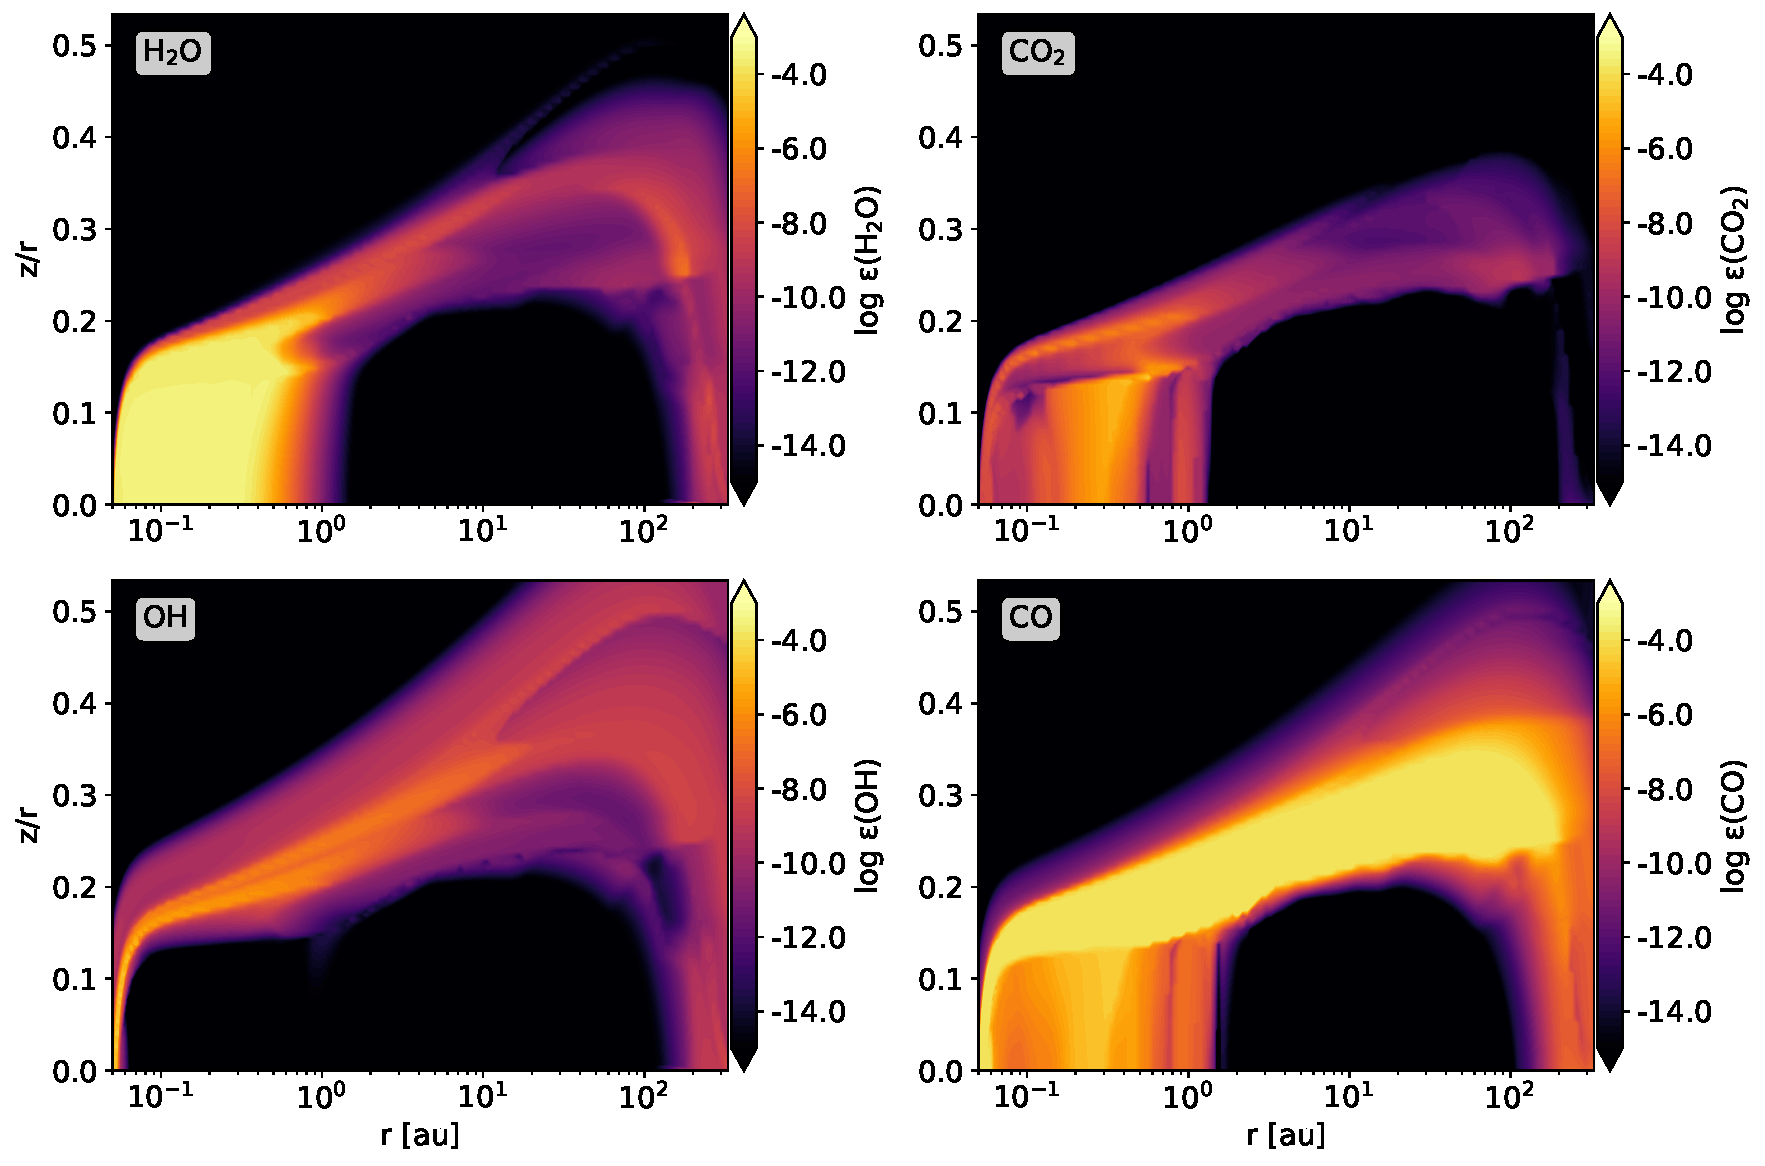
\includegraphics[width=\linewidth]{Figures/Abundance1.pdf}
    \caption{The distribution of H\2O, CO\2, OH, and CO across the disk of the fiducial model. The line origins of molecules in the wavelength range of JWST MIRI MRS are highlighted in cyan. The white contour line corresponds to a visual extinction of one. The horizontal axis shows the distance $r$ from the host star, and the vertical axis shows the height above the midplane $z$ divided by the radius $r$.}
    \label{fig: others distribution}
\end{figure}

In \autoref{fig: others distribution}, the distribution of H\2O, CO\2, OH, and CO is shown. A large reservoir of H\2O is visible between the host star and 1 au. In contrast, OH is only present in the atmosphere of the disk. This is caused by two effects. First, there is the formation of H\2O. OH can combine with molecular hydrogen to form H\2O (\ce{OH + H2 -> H2O + H}), which depletes the OH in the midplane of the disk. Secondly, there is photo-dissociation. In the upper parts of the atmosphere, there is less shielded from high-energy light such as UV and X-rays. This results in the dissociation of H\2O, forming OH. This results in most of the OH to be above a visual extinction ($A_V$) level of 1. CO is also present throughout the disk, especially in the warmer layers of the disk. In contrast, the abundance of CO\2 is very low at larger radii ($>$100 au) 
compared to the other molecules. There is a gap in the densities between 1 and 200 au. In these areas, the temperature drops below the freezing point of these molecules, and they are well shielded from UV radiation, resulting in the formation of ice. 

\begin{figure}[H]
    \centering
    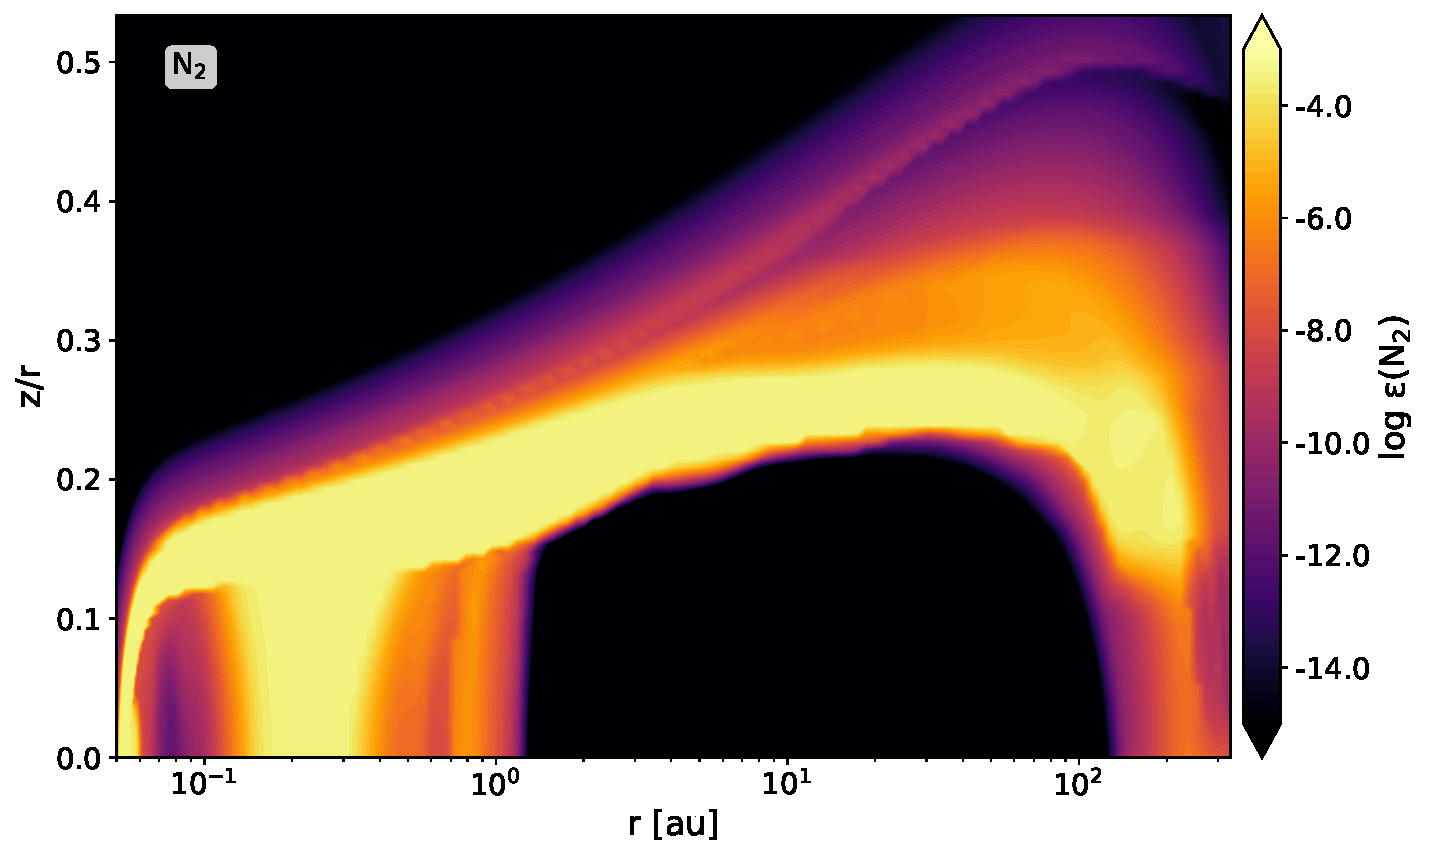
\includegraphics[width=.8\linewidth]{Figures/AbundanceN2.pdf}
    \caption{The distribution of N\2 across the disk of the fiducial model. The white contour line corresponds to a visual extinction of one. The horizontal axis shows the distance $r$ from the host star, and the vertical axis shows the height above the midplane $z$ divided by the radius $r$.}
    \label{fig: n2 distribution}
\end{figure}

The distribution of N\2 is shown in \autoref{fig: n2 distribution}. The abundance of N\2 is very high throughout the disk. This is expected as N\2 has a strong triple bond, which makes the molecules extremely stable and inert. However, this also means that most of the nitrogen in a disk is stored in N\2 molecules. This makes probing the nitrogen levels difficult as N\2 has no permanent dipole moment, making observations almost impossible.

\begin{figure}[H]
    \centering
    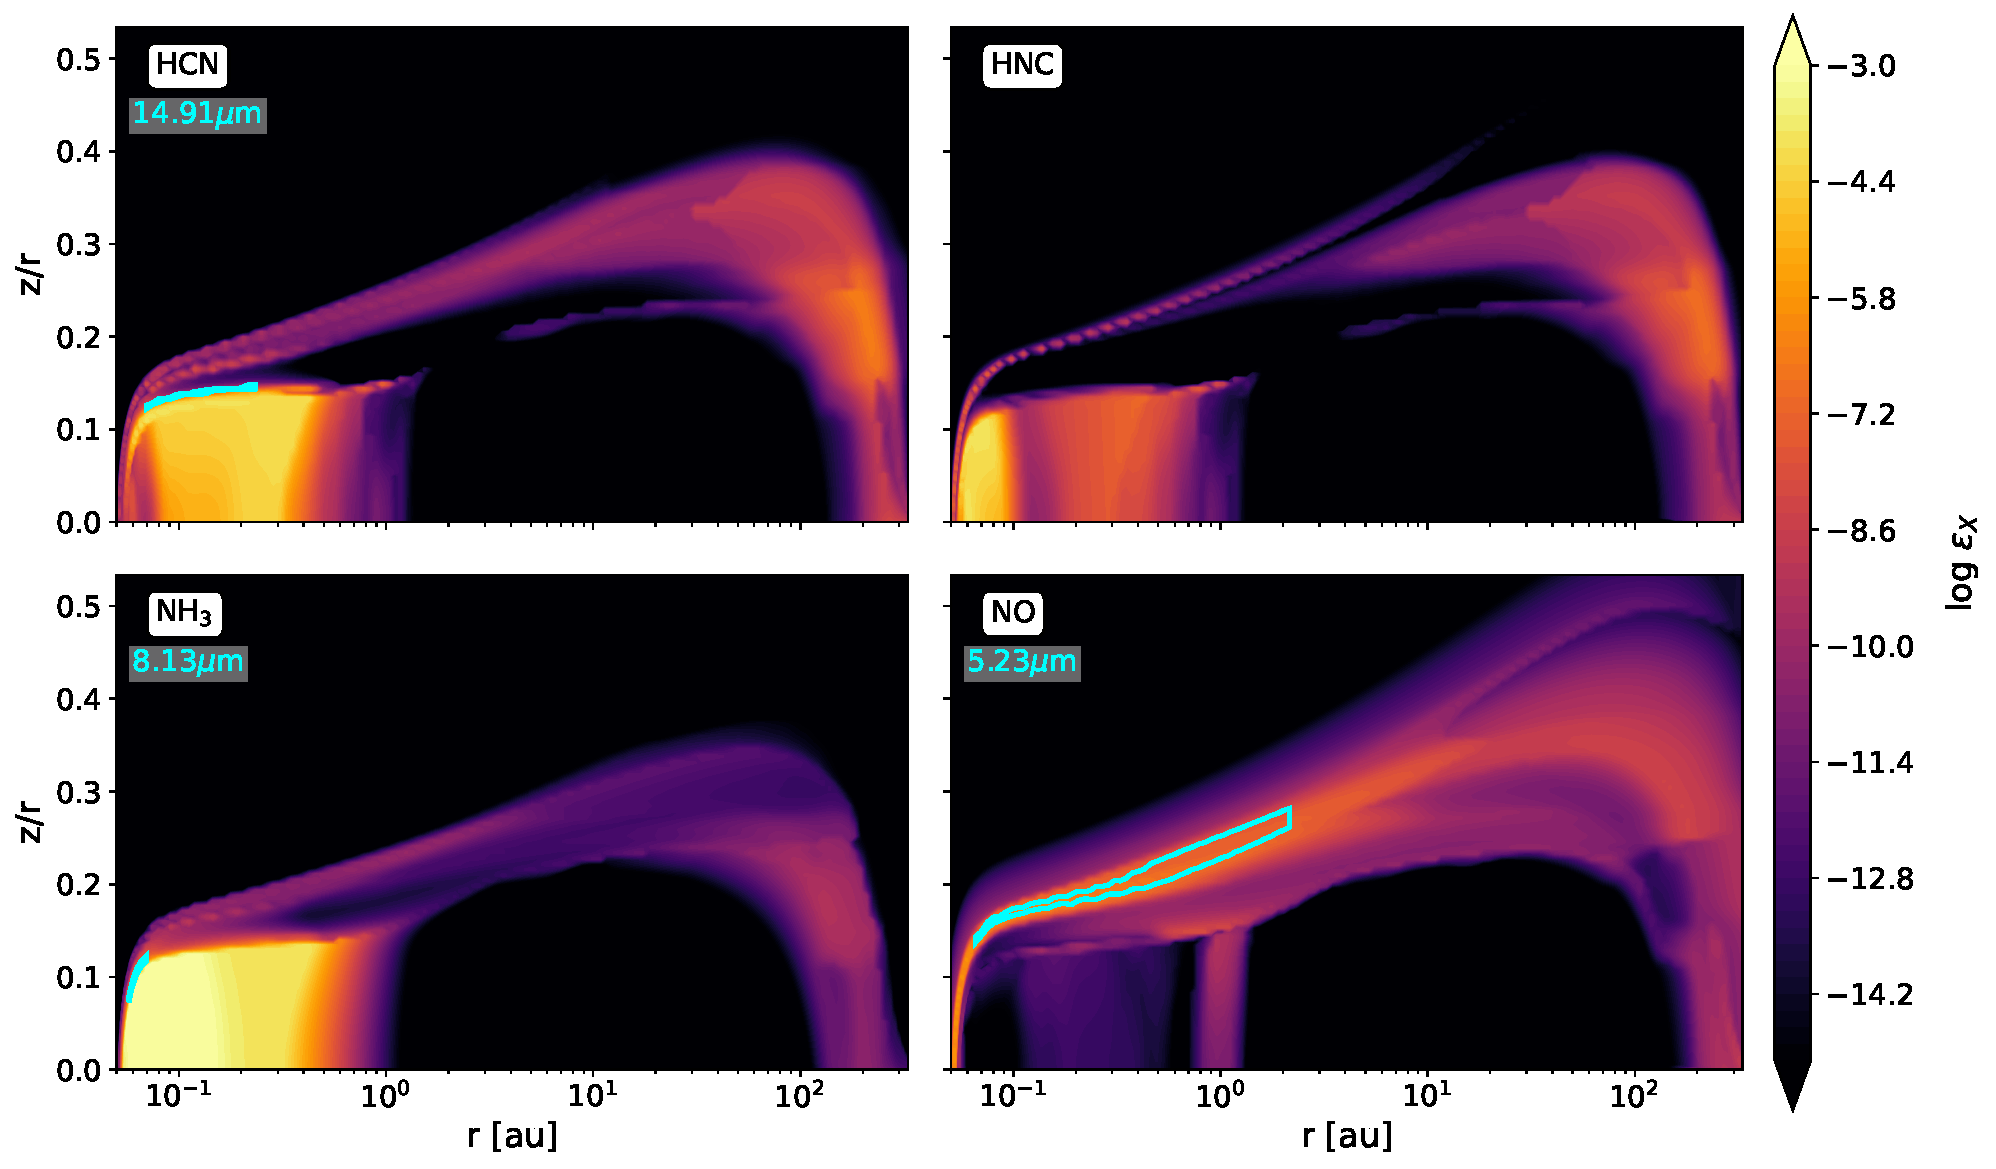
\includegraphics[width=\linewidth]{Figures/Abundance2.pdf}
    \caption{The distribution of HCN, HNC, NH\3, and NO across the disk of the fiducial model. The line origins of molecules in the wavelength range of JWST MIRI MRS are highlighted in cyan. The white contour line corresponds to a visual extinction of one. The horizontal axis shows the distance $r$ from the host star, and the vertical axis shows the height above the midplane $z$ divided by the radius $r$.}
    \label{fig: nitrogen distribution}
\end{figure}

Lastly, we inspected the distribution of nitrogen-bearing molecules: N\2 (\autoref{fig: n2 distribution}), HCN, HNC, NH\3, and NO (\autoref{fig: nitrogen distribution}). The density of the molecules changes a lot for different radii and heights. For example, in the region between 0.05 and 0.1 au, HCN decreases compared to the surrounding areas, but HNC increases in the same region. The abundance of NO is similar reservoir as OH, mostly in the surface of the disk. NH\3 is concentrated near the midplane of the disk. The NH\3 reservoir is mostly located below $A_V=1$, which would explain why it is difficult to detect.   
\newpage
\section{FLiTs Spectra}\label{sec: flits}
Consistent mid-infrared spectra were calculated using FLiTs for all the models in the grid. The resulting spectra are shown in \autoref{fig: all spectra}. There is a clear division in the shapes of the spectra. In the bottom left corner, six spectra have a strong C\2H\2 feature. These models also have a C/O ratio greater than one. The other models have strong water features and have a C/O ratio smaller than one. For our analysis, the spectra were split into two groups. One group containing the models with $C/O>1$ and the other containing the models with $C/O<1$.

\begin{figure}[H]
    \centering
    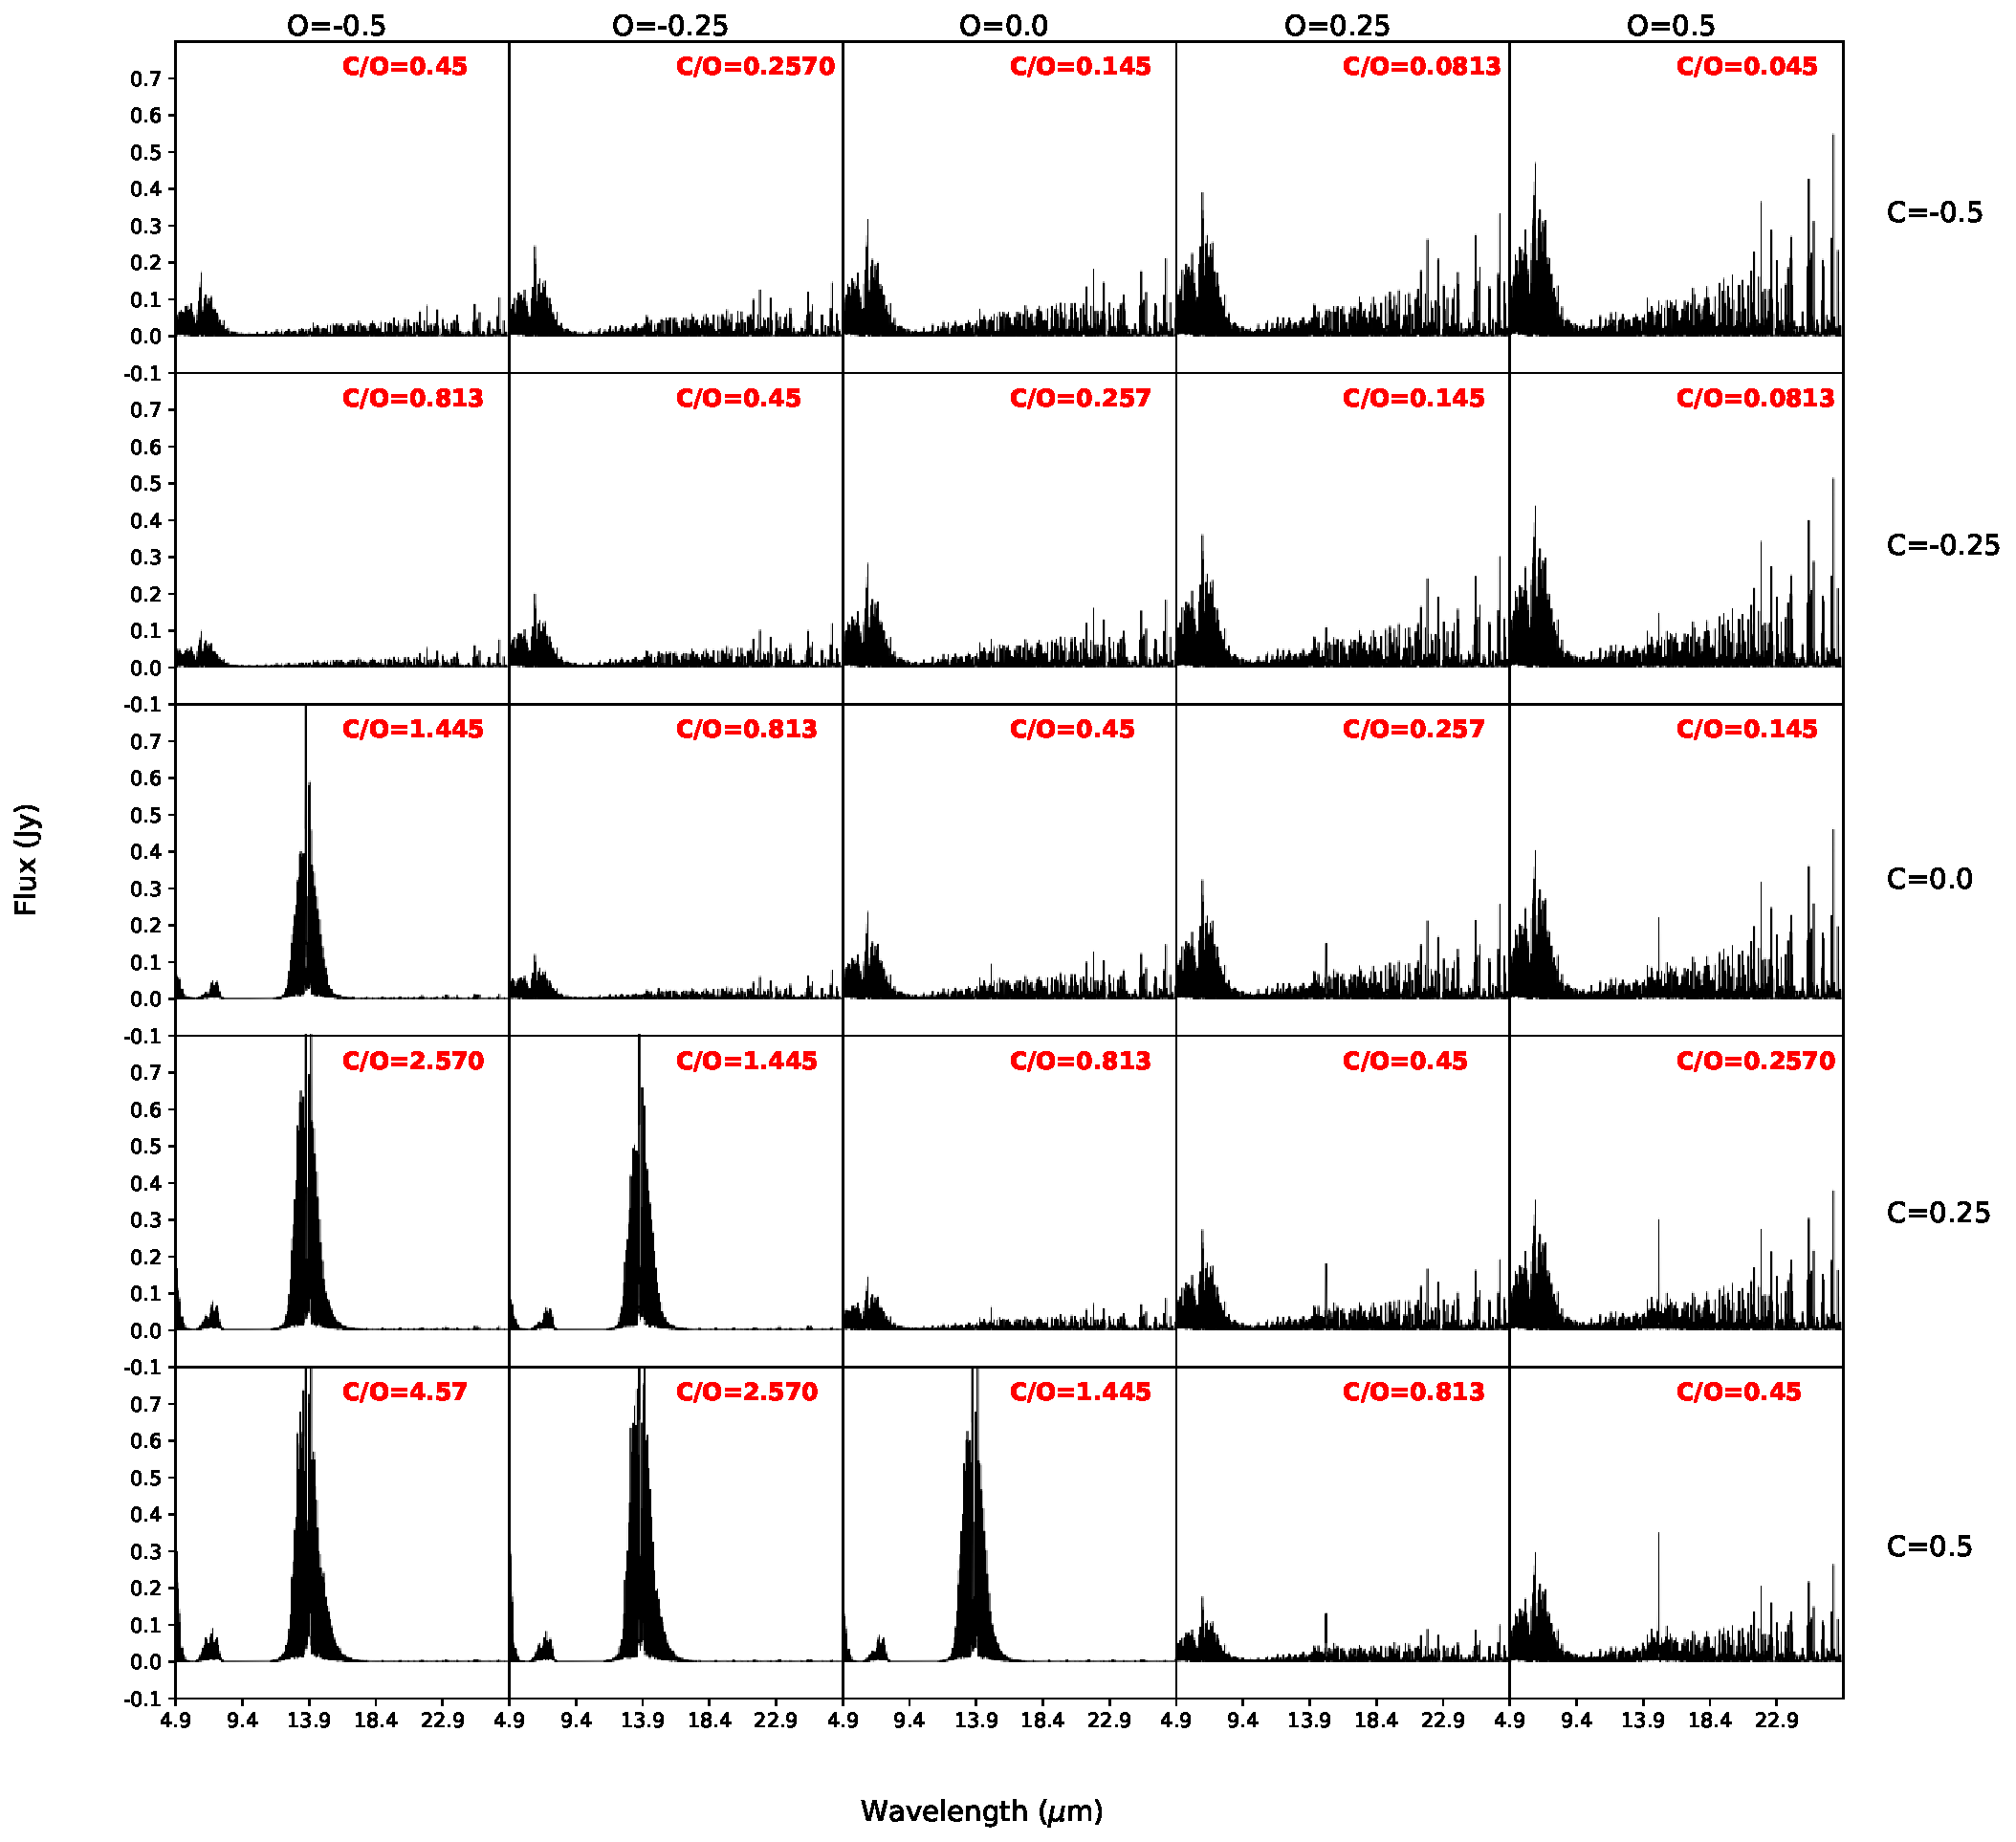
\includegraphics[width=.95\linewidth]{Figures/All_spectra.pdf}
    \caption{The simulated spectra of all the models in the model grid using FLiTs. On the horizontal axis, the O abundance varies from -0.5 to 0.5 with respect to the reference abundance. The C abundance varies from -0.5 to 0.5 with respect to the reference abundance from top to bottom. Some notable spectral features are labeled.}
    \label{fig: all spectra}
\end{figure}
\subsection{Total Flux across Grid}
The flux of the different molecules changes depending on the abundances of C and O. The total flux between 5 \textmu m and 28.5 \textmu m was calculated for all the molecules for which there are FLiTs spectra. \autoref{fig: Heatmaps1} shows the total flux for CO, CO\2, H\2O, and OH across the grid of models. The total flux for C\2H\2, HCN, NO, and NH\3 for all the models in the grid is shown in \autoref{fig: Heatmaps2}. 

\begin{figure}[H]
    \centering
    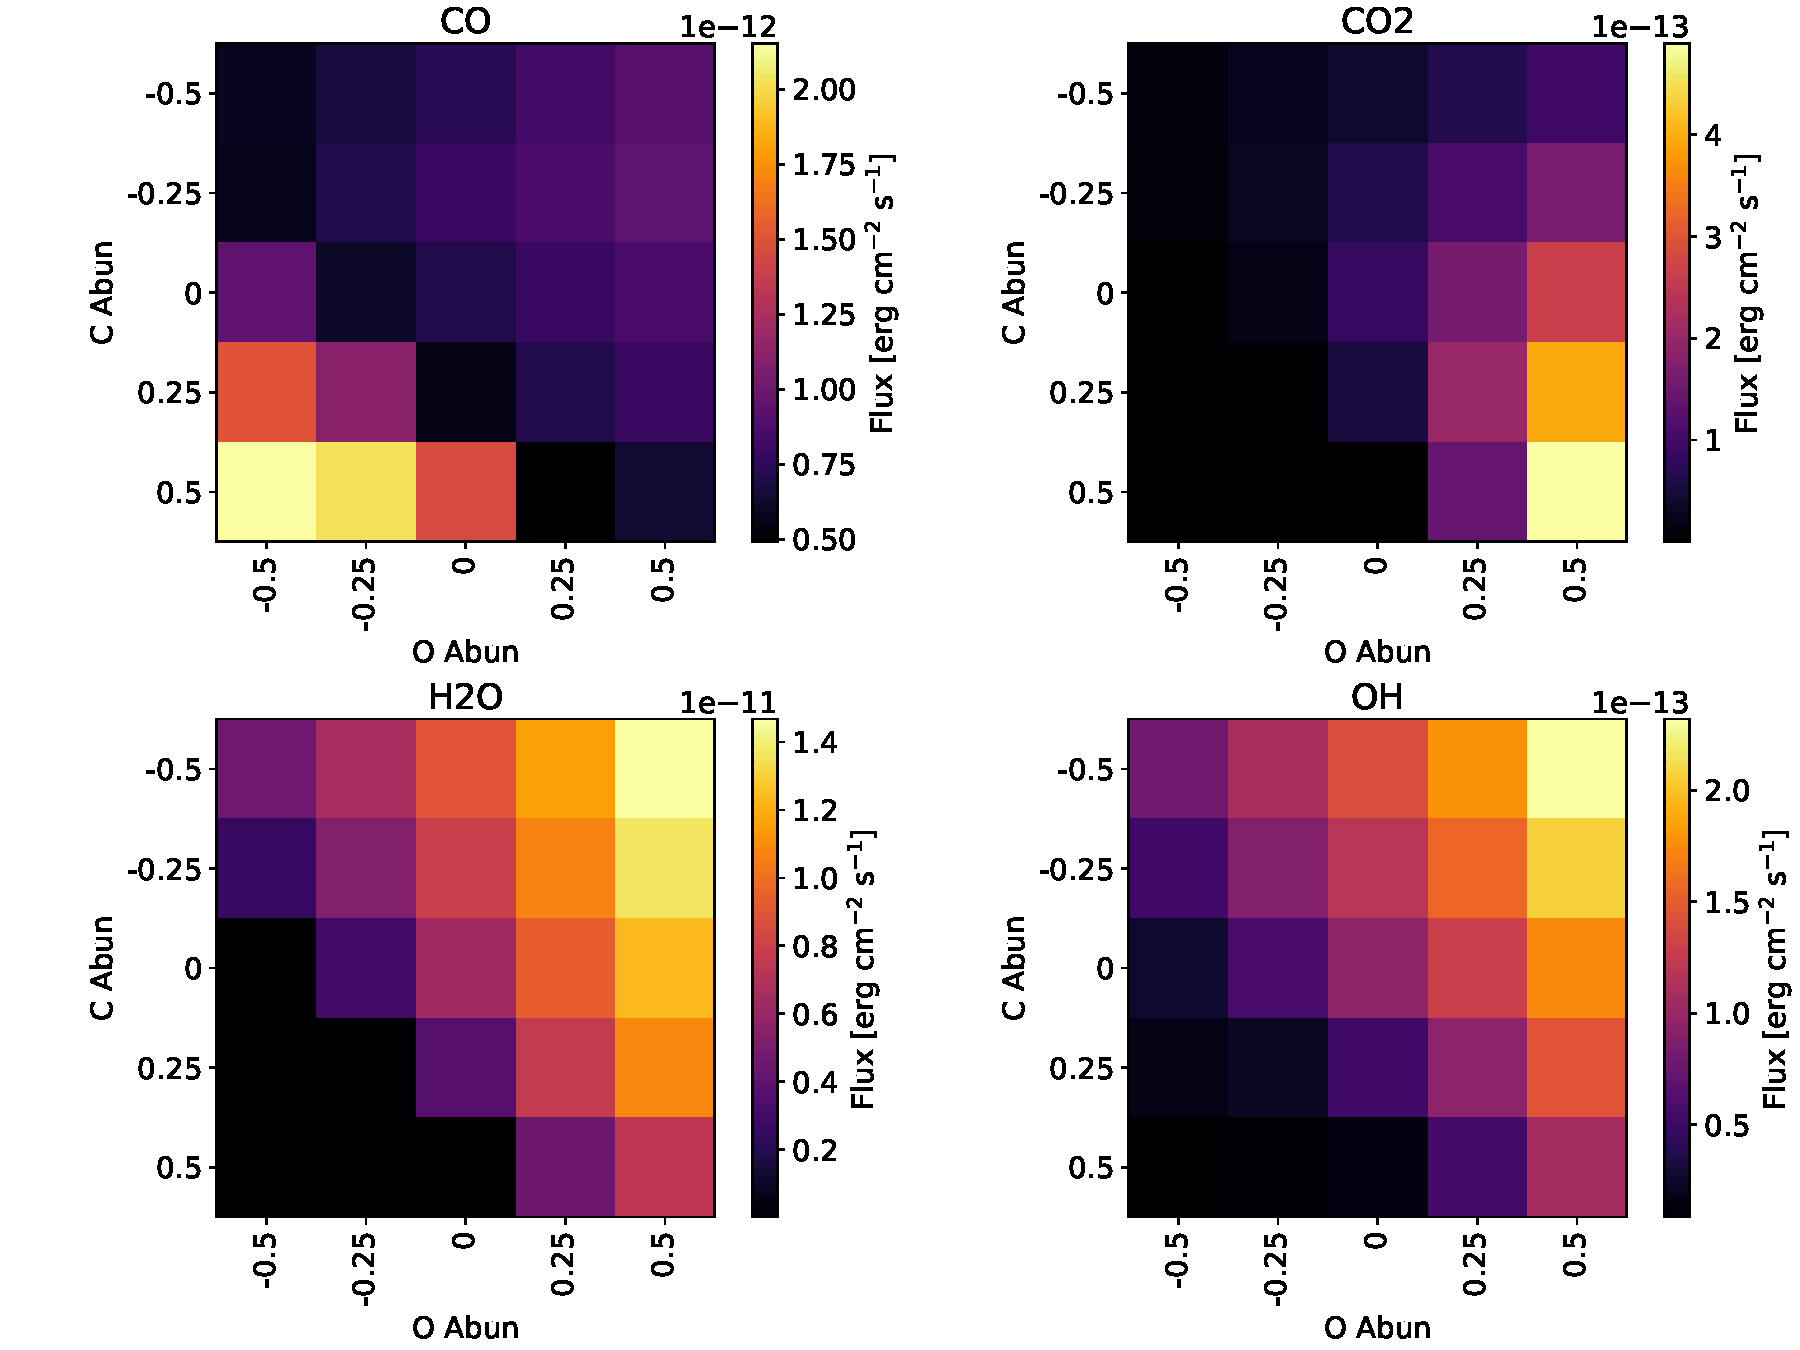
\includegraphics[width=\linewidth]{Figures/Heatmaps1.pdf}
    \caption{The total flux of CO, CO\2, H\2O, and OH for all the models in the grid.}
    \label{fig: Heatmaps1}
\end{figure}

The total flux of the molecules shown in \autoref{fig: Heatmaps1} shows patterns that are expected. The flux from H\2O and OH both increase as the abundance of C gets lower and the abundance of O gets higher. This is expected as this means that there is more O to form these compounds and less C, taking up O to form other compounds such as CO. The inverse is true for CO, where the flux increases as the abundance of C gets higher and the abundance of O gets lower. However, the flux of CO also increases for lower C abundance and higher O abundance, but to a lesser extent.  Much of the O gets stored in CO. When there is an increase in the O abundance on top of the higher C abundance, the flux of CO\2 also increases. 

\begin{figure}[H]
    \centering
    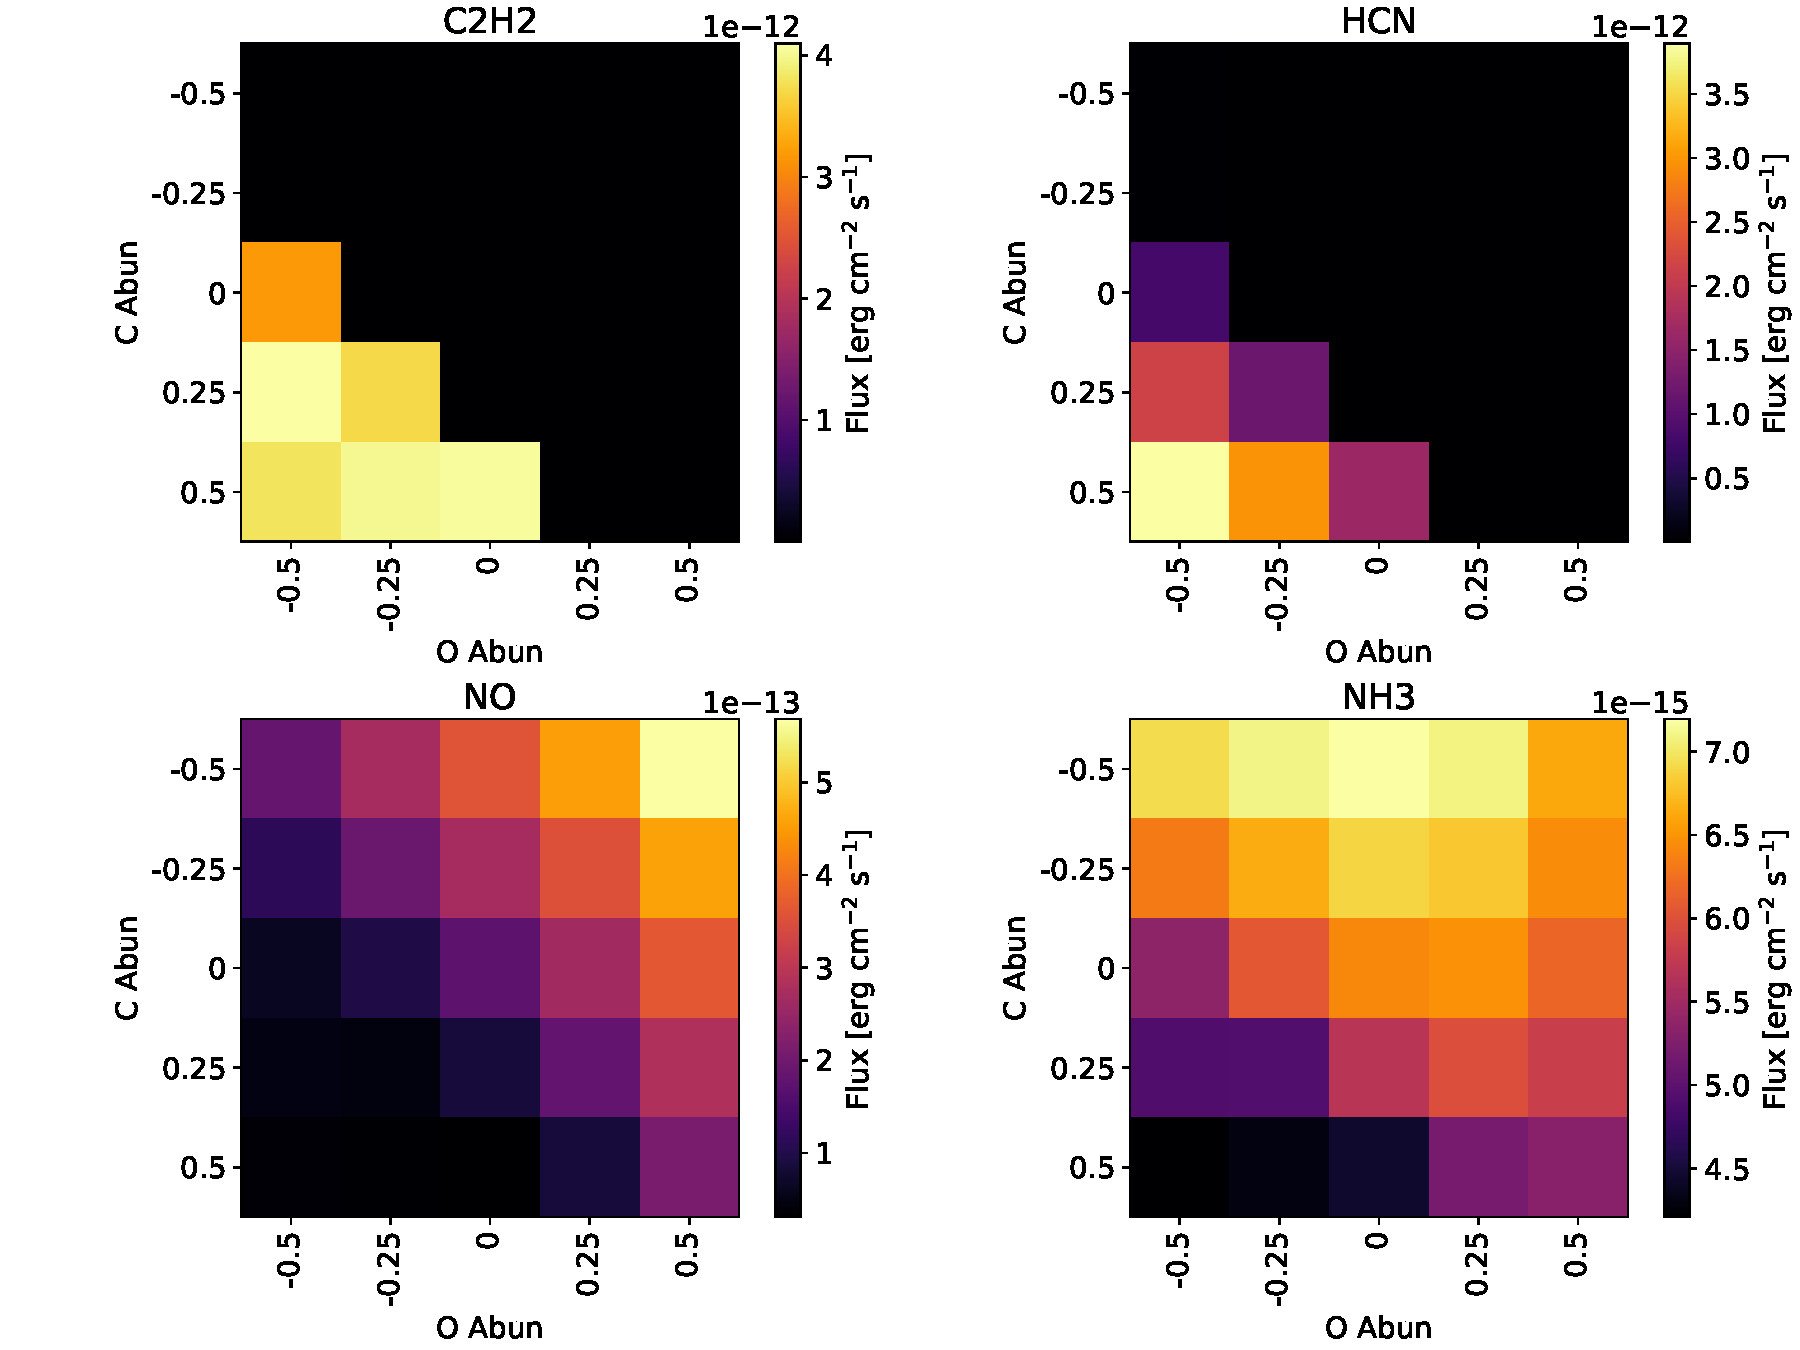
\includegraphics[width=\linewidth]{Figures/Heatmaps2.pdf}
    \caption{The total flux of C\2H\2, HCN, NO, and NH\3 for all the models in the grid.}
    \label{fig: Heatmaps2}
\end{figure}

In \autoref{fig: Heatmaps2}, it is clear that there is a large flux from C\2H\2 for the spectra that have a C/O ratio greater than one and barely any flux from the spectra that have a C/O ratio smaller than one. The HCN flux increases as C/O becomes larger, as this means there is more carbon available to store nitrogen in. In contrast, NO flux increases as C/O becomes smaller, as this means there is more O available. The flux of NH\3 generally increases as the C abundance gets lower. We hypothesize that the cause for this is the reactions that take place to form NH\3.
OH is an important component in the formation of NH\3. \textbf{CHECK CHEMISTRY}

\ce{NH2+ + OH -> NH3 + O+}

\textbf{MORE REACTIONS}\\
Furthermore, there could be some competition with HCN, where more N is locked in HCN when the C abundance is larger. 

We also used a ProDiMo model with solar abundances, including the N abundance.

\begin{figure}
    \centering
    \includegraphics[width=0.5\linewidth]{solarabund+enhanced}
    \caption{The simulated spectra for the model with solar abundances (top) and the model with enhanced nitrogen (bottom). }
    \label{fig:enter-label}
\end{figure}



\subsection{Regions of Interest}
Next, we investigated regions in the spectrum that could help us detect NO and NH\3. The model grid was split into two groups, as noted in \autoref{sec: Prodimo output}. One group has C/O smaller than one, and the other greater. The spectra were split into 0.01 \textmu m spectral windows, and for each window, the molecule that had the strongest emissions compared to the other molecules was determined. The result is shown in \autoref{fig: classes}.

% \begin{figure}[H]
%     \centering
%     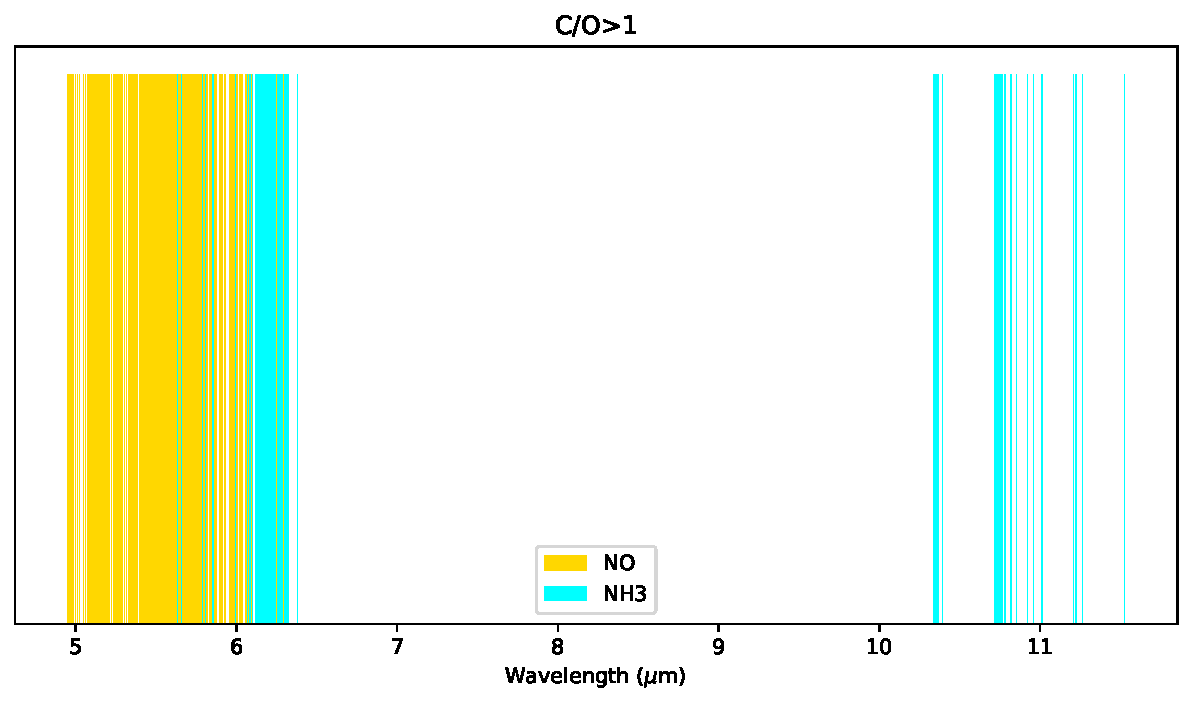
\includegraphics[width=\linewidth]{Figures/ClassificationCOgt0.pdf}
%     \caption{The regions of the spectrum where NO and NH\3 emission are the  strongest compared to other molecular emission in the models that have a C/O greater than one}
%     \label{fig: class>1}
% \end{figure}

% \begin{figure}[H]
%     \centering
%     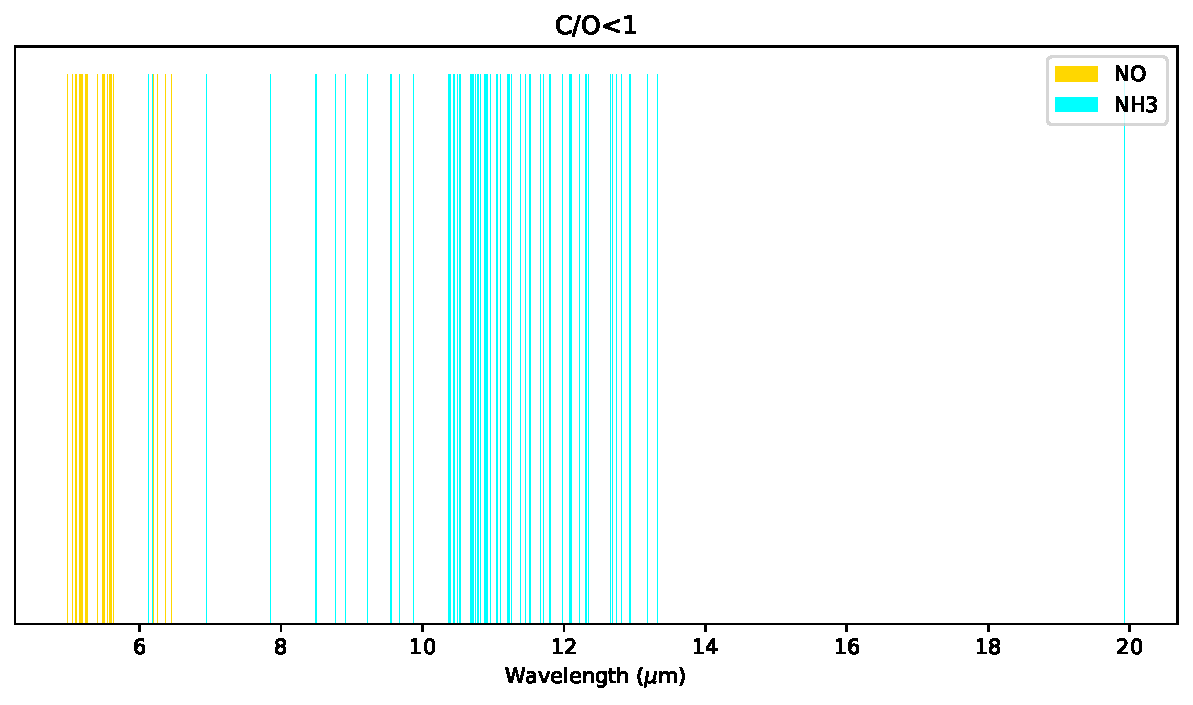
\includegraphics[width=\linewidth]{Figures/ClassificationCOst0.pdf}
%     \caption{The regions of the spectrum where NO and NH\3 emission are strongest in the models that have a C/O smaller than one}
%     \label{fig: class<1}
% \end{figure}

\begin{figure}[H]
    \centering
    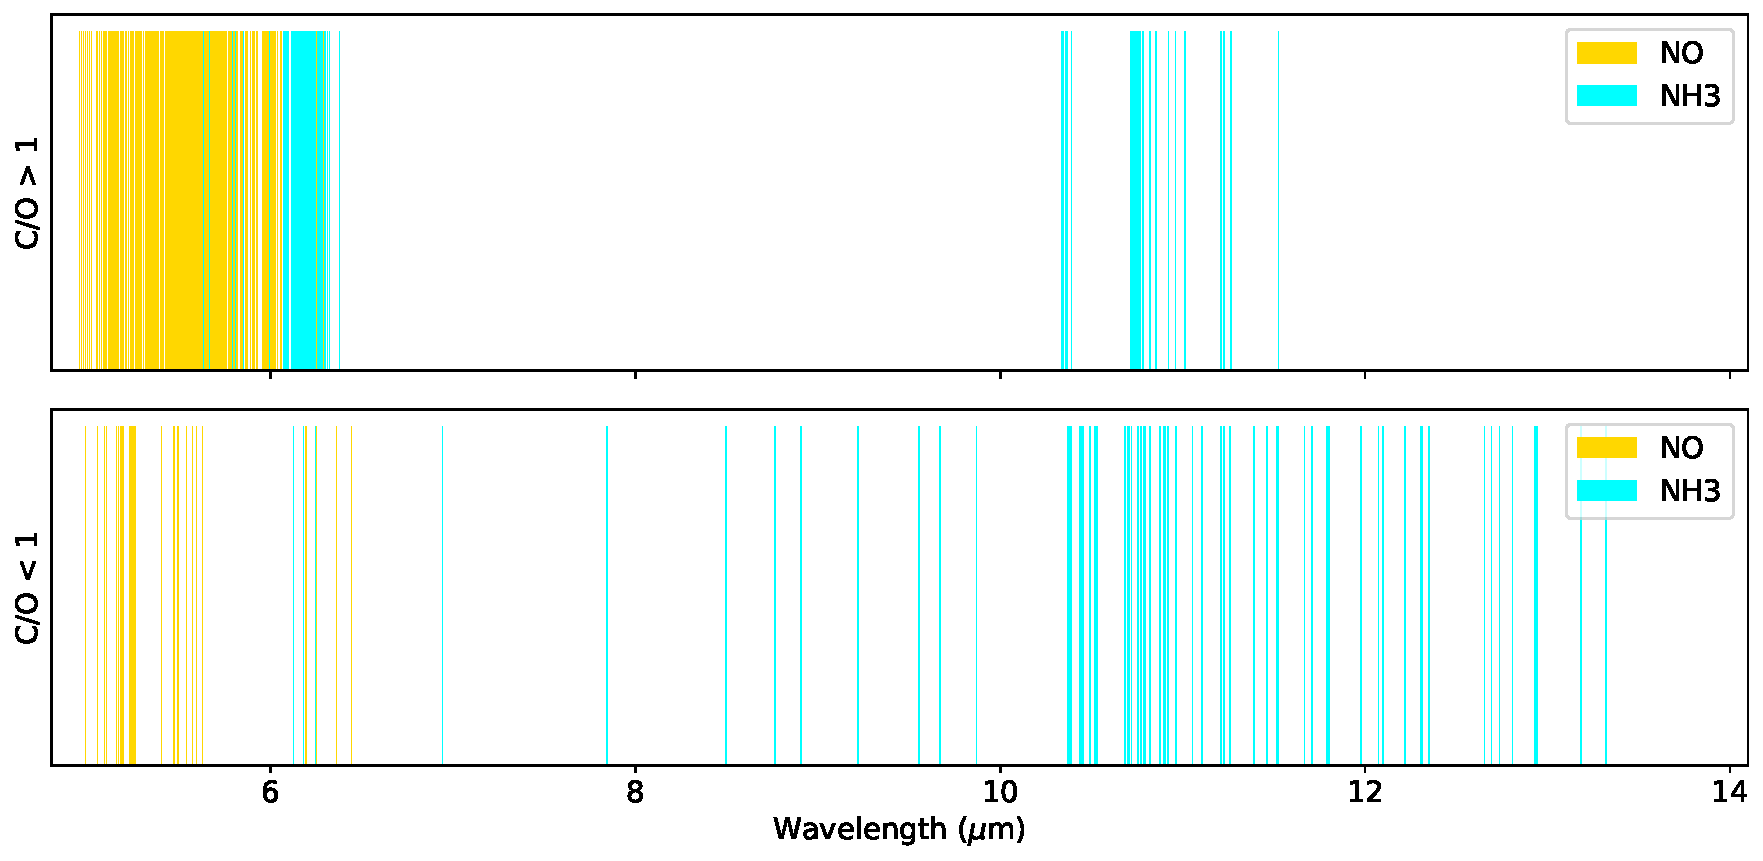
\includegraphics[width=\linewidth]{Figures/ClassificationCO.pdf}
    \caption{The regions of the spectrum where NO and NH\3 emission are strongest in the models for models that have a C/O greater than one (top) and smaller than one (bottom)}
    \label{fig: classes}
\end{figure}

In the top row of \autoref{fig: classes} corresponding to the model with a C/O ratio greater than one, it is visible that the region between 4.9\textmu m and 6 \textmu m has many spectral regions where the emission from NO is the strongest. NH\3 has the brightest emission compared to all other molecules between 6 \textmu m and 6.4 \textmu m. Between 10 \textmu m and 12 \textmu m, there are some smaller regions where NH\3 is the strongest. In contrast, in the bottom row of \autoref{fig: classes} corresponding to the model with a C/O ratio smaller than one, the spectral regions where NO or NH\3 emission is strongest are more barren. The NO emission regions are no longer the strongest anymore, and neither is the NH\3 emission region between 6 \textmu m and 6.4 \textmu m. This is caused by the presence of H\2O lines, which completely outshine the NO and NH\3 emission in this region. The most promising region for NH\3 is now between 9.5 \textmu m and 13 \textmu m with a few small windows in which the emission of NH\3 is the strongest.

The spectral regions where the emission of NO or NH\3 is the strongest, as shown in \autoref{fig: classes}, were examined to evaluate the detectability of NO and NH\3. For this, the fiducial model was used to represent the spectra with $C/O<1$, and the model with abundances C+0.25 and O-0.25 was used to represent the spectra with $C/O>1$.

\begin{figure}[H]
    \centering
    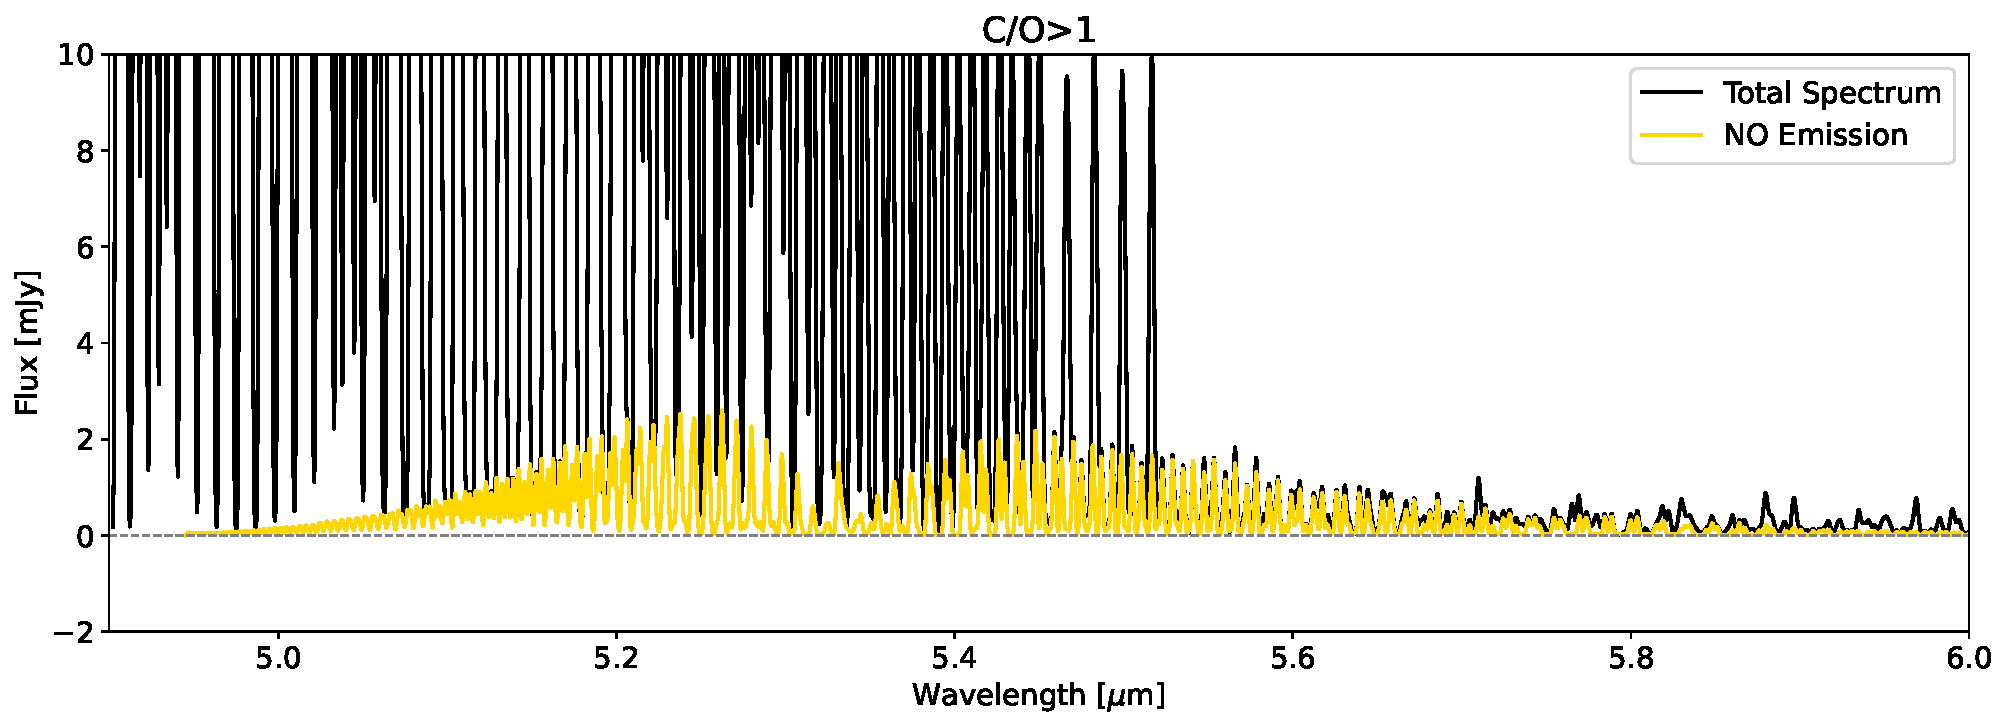
\includegraphics[width=\linewidth]{Figures/NO_region.pdf}
    \caption{A zoomed-in region of the spectrum of the fiducial model between 4.9 \textmu m and 6 \textmu m where NO emission is strongest.}
    \label{fig: NO region}
\end{figure}

In the region shown in \autoref{fig: NO region}, a bright CO spectral feature is present. This makes the detection of NO difficult. However, the CO lines become more barren around 5.45 \textmu m and disappear above 5.5 \textmu m, which makes the emission of NO the only emission in this region. 

\begin{figure}[H]
    \centering
    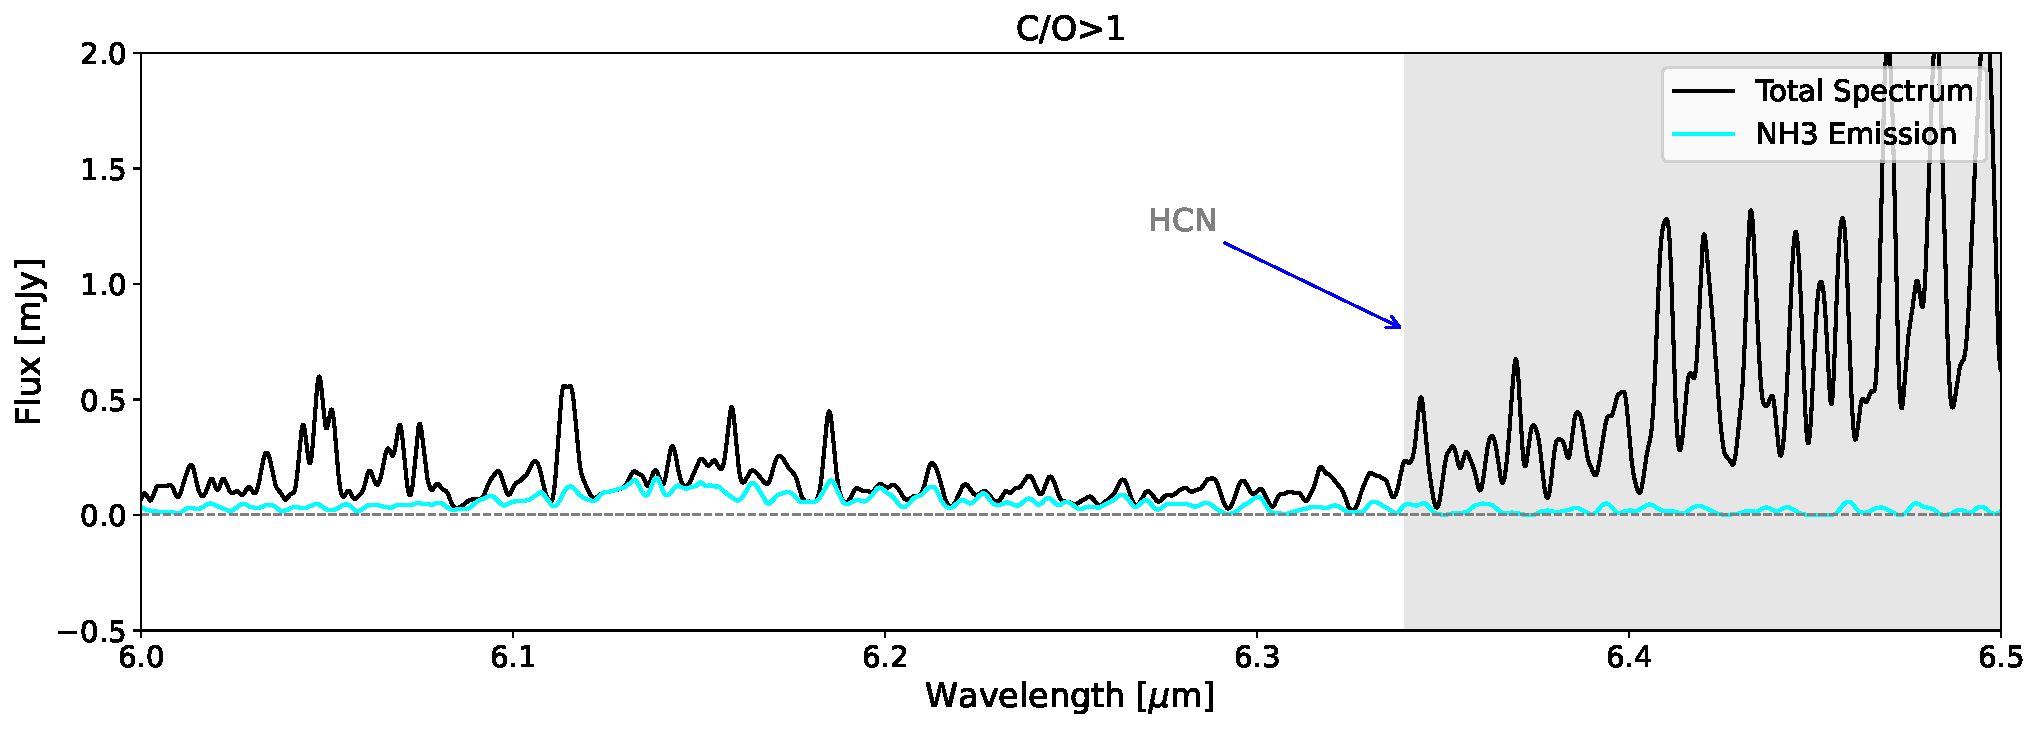
\includegraphics[width=\linewidth]{Figures/NH3_region1.pdf}
    \caption{A zoomed-in region of the spectrum of the model with C+0.25 and O-0.25 between 6 \textmu m and 6.5 \textmu m where NH\3 emission is strongest.}
    \label{fig: NH3 region 1}
\end{figure}

\autoref{fig: NH3 region 1} shows that the emission of NH\3 makes up a large part of the spectrum in this region. There are a few lines from other molecules and a bright HCN feature starting around 6.35 \textmu m.

\begin{figure}[H]
    \centering
    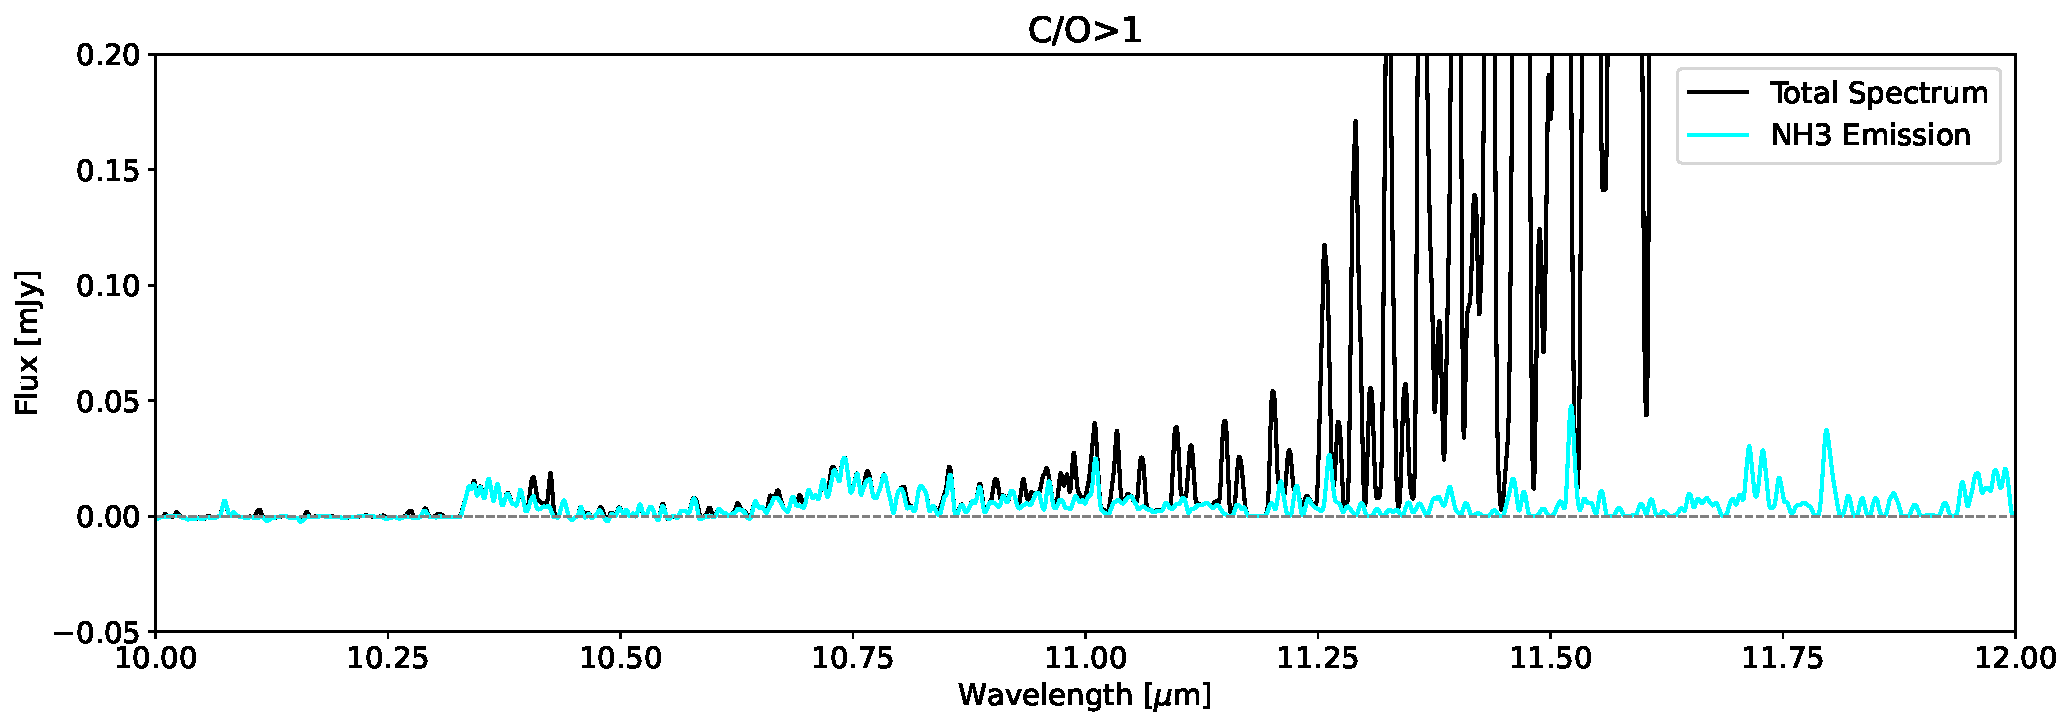
\includegraphics[width=\linewidth]{Figures/NH3_region2.pdf}
    \caption{A zoomed-in region of the spectrum of the model with C+0.25 and O-0.25 between 10 \textmu m and 12 \textmu m where NH\3 emission is strongest.}
    \label{fig: NH3 region 2}
\end{figure}

The spectral region shown in \autoref{fig: NH3 region 2} has similar features to the region shown in \autoref{fig: NH3 region 1}. This region also has a part where the NH\3 emission makes up most of the spectrum, with a few lines from other molecules. Similarly, bright lines are coming from C\2H\2 and HCN starting around 11.25 \textmu m.

\begin{figure}[H]
    \centering
    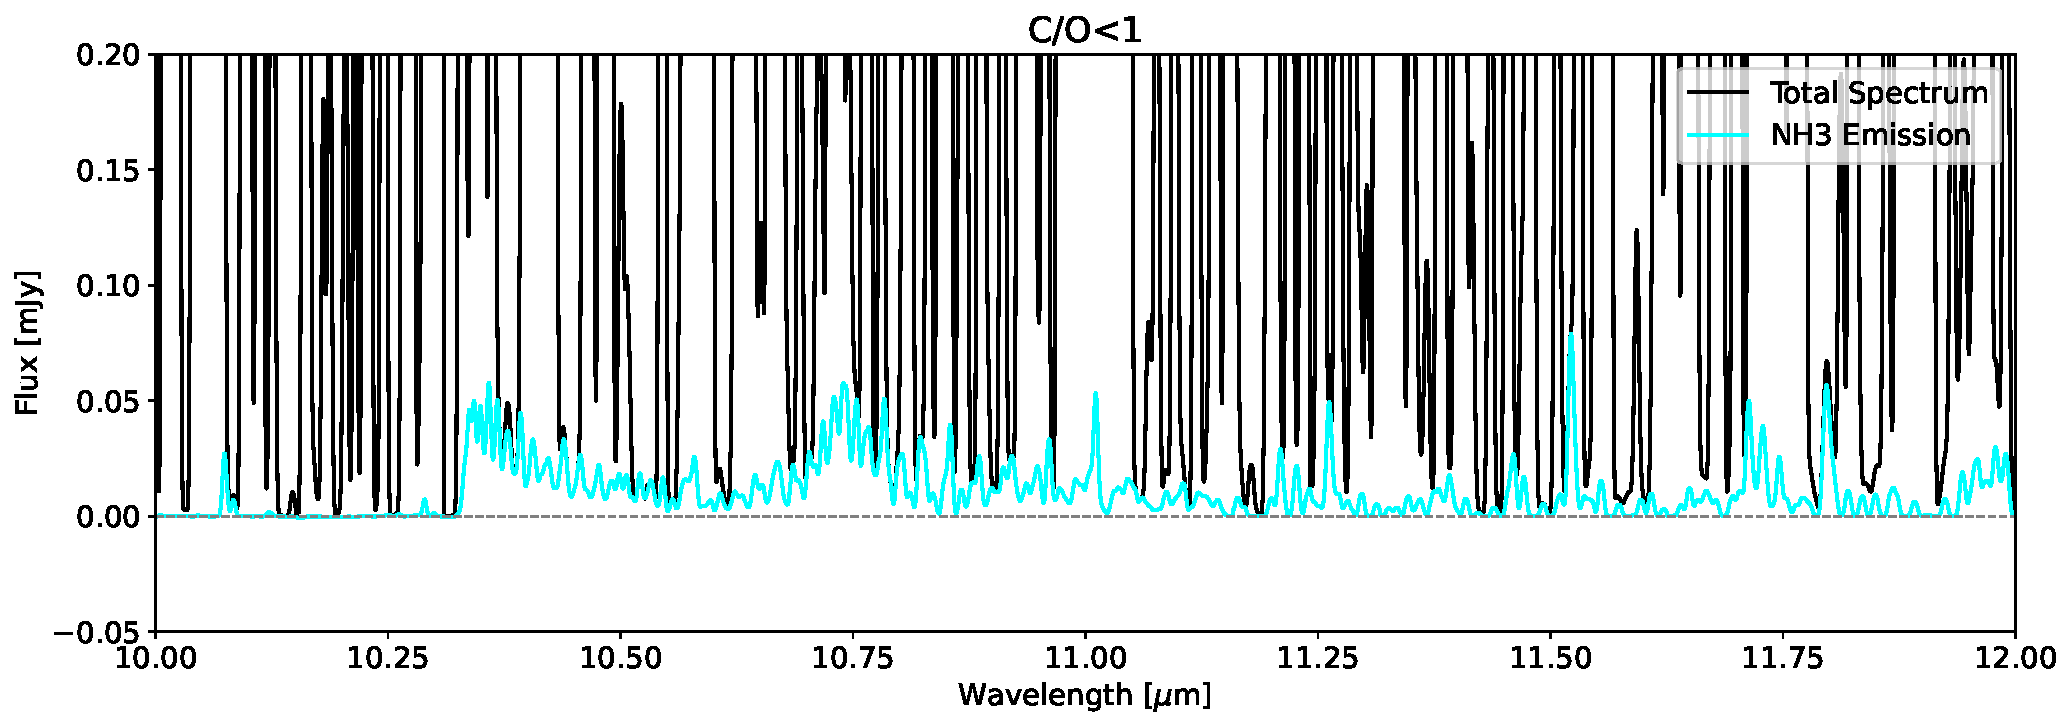
\includegraphics[width=\linewidth]{Figures/NH3_region3.pdf}
    \caption{A zoomed-in region of the spectrum of the fiducial model between 10 \textmu m and 12 \textmu m where NH\3 emission is strongest.}
    \label{fig: NH3 region 3}
\end{figure}

All of the regions shown up until this point were for the fiducial model, which has $C/O<1$. For the model with $C/O>1$, NO has no more regions where it is the brightest, and there are fewer windows where NH\3 is the brightest. Some of these windows are shown in \autoref{fig: NH3 region 3}. The emission from H\2O is much stronger than that of NH\3, making it undetectable. There are some regions (e.g., at 11.8 \textmu m) where the emission from NH\3 falls between lines from H\2O. 

\begin{figure}[H]
    \centering
    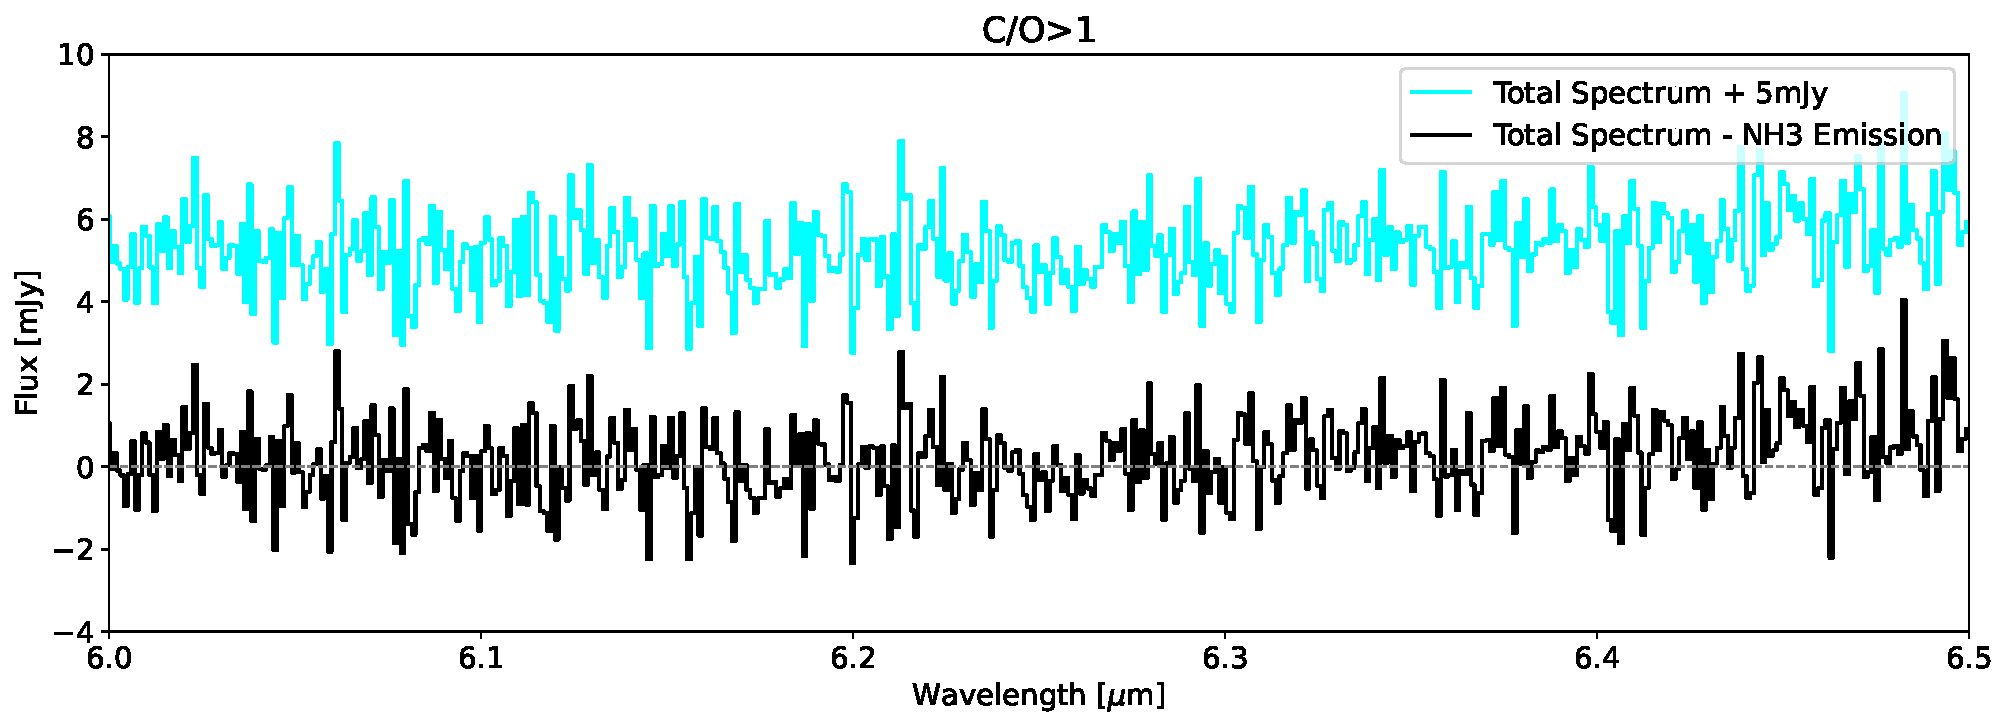
\includegraphics[width=\linewidth]{Figures/AddNoise.pdf}
    \caption{A zoomed-in region of the spectrum of the model with C+0.25 and O-0.25 between 6 \textmu m and 6.5 \textmu m where NH\3 emission is strongest. A Gaussian noise corresponding to an SNR of 300 was added.}
    \label{fig: add noise}
\end{figure}

The spectral regions shown in \autoref{fig: NO region}, \autoref{fig: NH3 region 1}, \autoref{fig: NH3 region 2}, and \autoref{fig: NH3 region 3} are without noise. When Gaussian noise corresponding to SNR = 300 is added to the spectral region shown in \autoref{fig: NH3 region 1}, the emission NH\3 becomes difficult to detect as the noise level is much higher than the emission from NO. This is shown in  \autoref{fig: add noise}, where the emission with and without NH\3 emission is virtually identical.

\section{Molecule Detection}
In \autoref{fig: add noise}, it is difficult to distinguish the NH\3 and NO from the spectrum visually. However, cross-correlation is a technique that can be used to find such weak signals. In calculating the cross-correlation, we used the average spectrum for each species of all the models in the model grid and normalized them. This template was then used to cross-correlate with the full spectrum. The cross-correlation of the H\2O template with the spectrum of the fiducial model is shown in \autoref{fig: crosscorr}. The peak signals that H\2O is present in the spectrum. 

\begin{figure}[H]
    \centering
    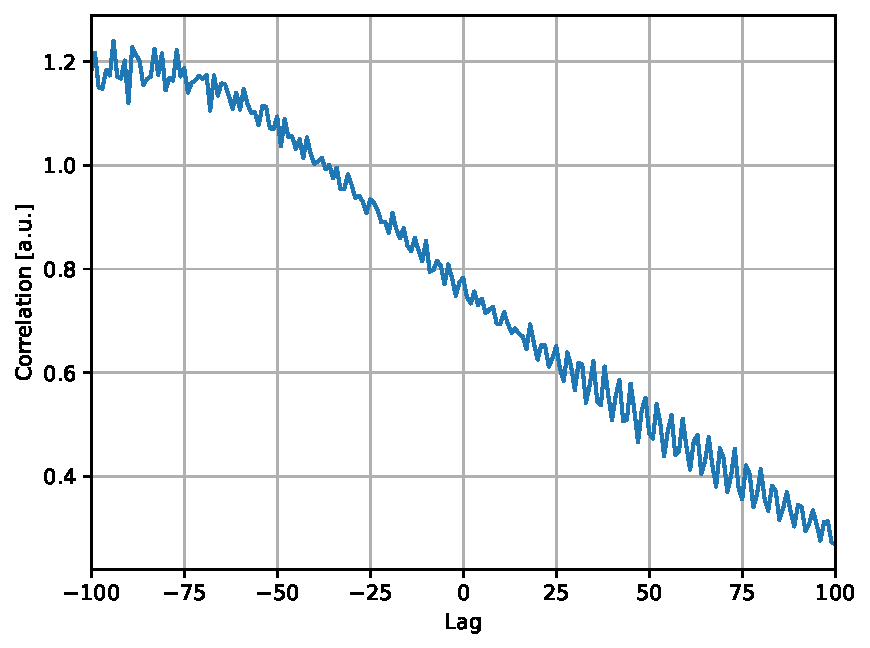
\includegraphics[width=.5\linewidth]{Figures/Cross-Correlation.pdf}
    \caption{The cross-correlation of the H\2O template with the spectrum the fiducial model}
    \label{fig: crosscorr}
\end{figure}

When this method was applied to the fiducial model and model C+0.25 O-0.25, we got the detections shown in \autoref{tab: combined_detections}. To check whether the cross-correlation technique can give false positives, the previous step was repeated, but this time with the emission for the molecule that is checked removed from the spectrum.

\begin{table}[!ht]
\centering
\resizebox{\textwidth}{!}{
\begin{tabular}{|l|ccc|ccc|}
\hline
\textbf{Molecule} & \textbf{A: Detected} & \textbf{A: Residual} & \textbf{A: Confirmed} & \textbf{B: Detected} & \textbf{B: Residual} & \textbf{B: Confirmed} \\
\hline
C$_2$H$_2$ & No  & No  & --           & Yes & No  & \ding{51} \\
% CH$_4$     & No  & No  & --           & No  & No  & --        \\
CO         & Yes & No  & \ding{51}    & Yes & No  & \ding{51} \\
CO$_2$     & Yes & No  & \ding{51}    & No  & No  & --        \\
H$_2$O     & Yes & No  & \ding{51}    & No  & No  & \ding{51} \\
HCN        & No  & No  & --           & Yes & No  & \ding{51} \\
NH$_3$     & No  & No  & --           & No  & No  & --        \\
NO         & No  & No  & \ding{51}    & No  & No  & \ding{51} \\
OH         & Yes & No  & \ding{51}    & No  & No  & --        \\
\hline
\end{tabular}
}
\caption{Molecular detections in the spectrum of the fiducial model (A) and the model with C+0.25 and O-0.25 (B) before and after subtracting molecular emission. A confirmed detection (\ding{51}) indicates that the molecule is detected in the full spectrum. A molecular emission is considered present in the full spectrum when the integrated flux over the wavelength range is greater than the integrated flux of a flat continuum at 0.1 mJy over the wavelength range.}
\label{tab: combined_detections}
\end{table}

In \autoref{tab: combined_detections}, the cross-correlation technique does not result in any false positives. However, the emission from NH\3 is too weak to count as present in the spectrum, and although NO is bright enough, it is not being detected using this technique. 

As some of the flux of a species overlaps with the flux emitted by other species, it would make detection easier if the emissions of the other species were removed. This was done with the simulated data, as the simulation produced the spectra of the individual species. To test this, the cross-correlation technique was applied to only the emission of NO and NH\3 separately, with the associated noise added. Repeating this 100 times with different random noise for every model in the model grid gave a detection rate of 100\% and 23.8\% for NO and NH\3, respectively.  Especially the region where NO is emitted is of interest, as the only other species that emit in that range are CO and H\2O. Removing the flux of CO and H\2O for the fiducial gives the spectrum shown in \autoref{fig: H2O and CO removed}.

\begin{figure}[H]
    \centering
    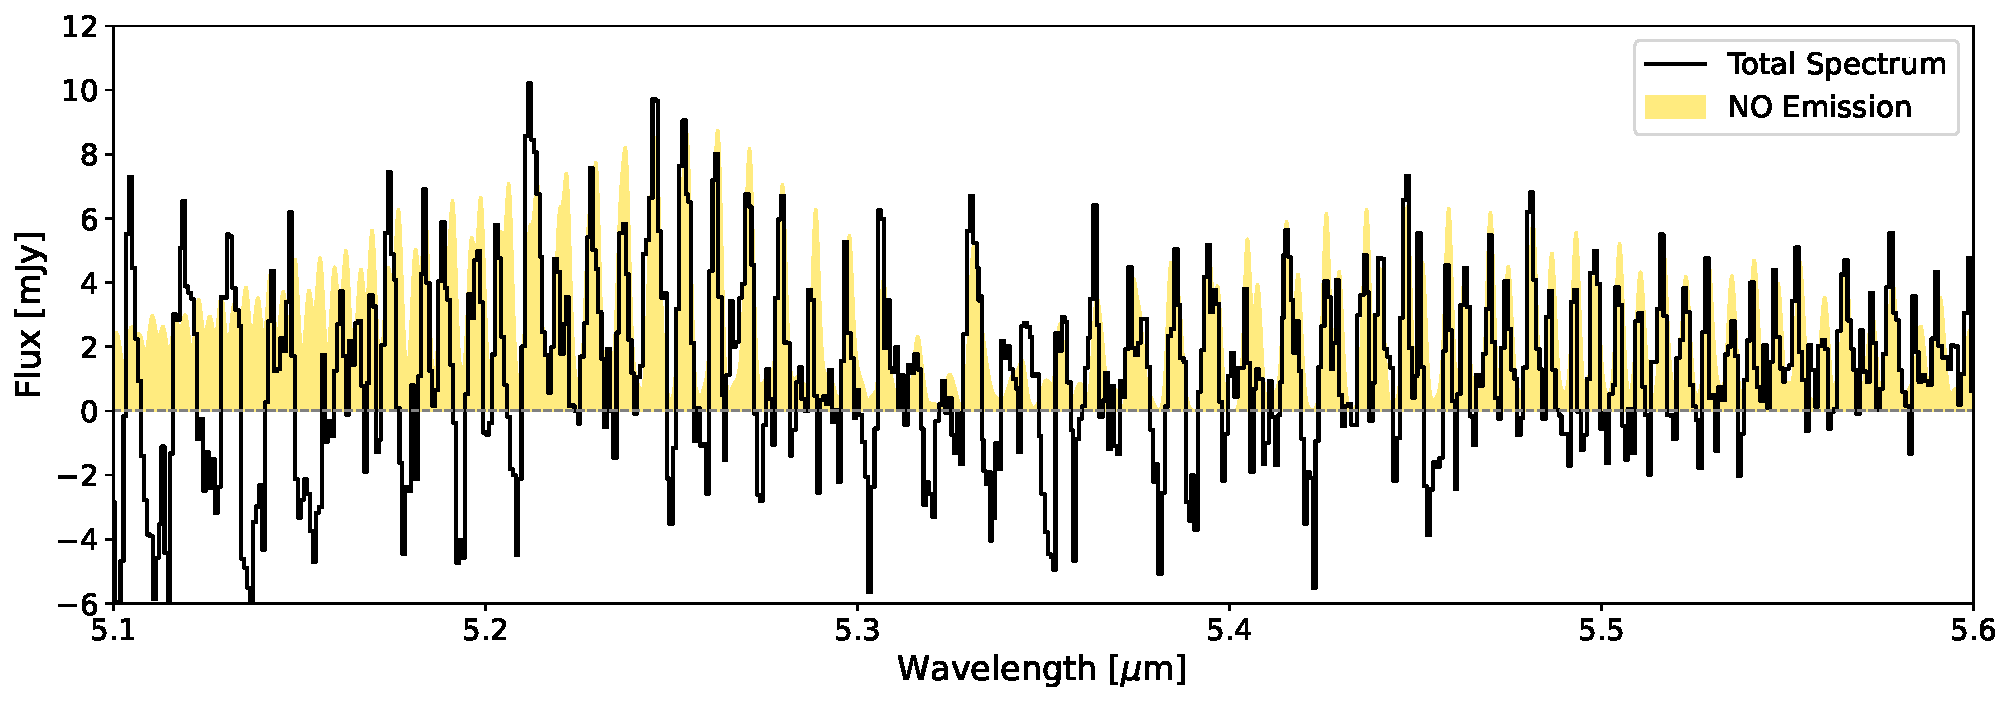
\includegraphics[width=\linewidth]{Figures/H2O_CO_removed.pdf}
    \caption{A zoomed-in region of the spectrum of the fiducial model with added noise corresponding to SNR = 300 between 5.1 \textmu m and 5.6 \textmu m. The emission of both H\2O and CO has been removed.}
    \label{fig: H2O and CO removed}
\end{figure}

In \autoref{fig: H2O and CO removed}, the NO emission becomes visible when the emission of H\2O and CO is removed. However, the noise causes large parts of the spectrum sizes of the peaks to vary, but the repetitive pattern of the NO emission is largely preserved. 

\section{Application of Detection Methods to JWST Observations}
After the confirmation that this technique is valid on the simulated spectra and does not result in false positives, it was applied to real data.

\subsection{Molecule Detection}\label{subsec: Molecule Detection}
Using the templates generated from the emission of the species for all the ProDiMo models in the grid, we cross-correlated the templates with the observed spectra. The results of this are shown in \autoref{tab: realdata}.

\begin{table}[H]
\centering
\begin{tabular}{|l|ccc|}
\hline
\textbf{Molecule} & \textbf{GWLup} & \textbf{Sz98} & \textbf{V1094Sco} \\ \hline
C\2H\2            & Detection      & Non-detection & Detection         \\
% CH4             & Non-detection  & Non-detection & Non-detection     \\
CO              & Detection      & Detection     & Detection         \\
CO\2             & Detection      & Detection     & Detection         \\
H\2O             & Detection      & Detection     & Detection         \\
HCN             & Detection      & Detection     & Detection         \\
NH\3             & Non-detection  & Non-detection & Non-detection     \\
NO              & Non-detection  & Non-detection & Non-detection     \\
OH              & Detection      & Detection     & Detection         \\ \hline
\end{tabular}

\caption{The detection of different molecules in the spectra of GWLup, Sz98, and V1094Sco using cross-correlation.}
\label{tab: realdata}
\end{table}

The detections in \autoref{tab: realdata} align with what is expected from the detected molecules in the simulated spectra and with the detections by \cite{Grant_2023}, and \cite{Gasman_2023}. In other words, detection for all molecules, except NO and NH\3, is directly possible. 

As discussed in \autoref{subsec: Molecule Detection}, the detection of NO emission becomes possible when removing all emission from H\2O and CO.
To remove the H\2O and CO emission from the observations, we used LTE models to fit CO and H\2O in the region between 4.9 \textmu m and 6.5 \textmu m to the observations. This region was selected as it mostly contains emission from just H\2O, CO, and NO. The resulting fits are shown in \autoref{fig: fits}. In \autoref{app: chi square}, the $\chi^2$-maps of the fits are shown.

\begin{figure}[H]
    \centering
    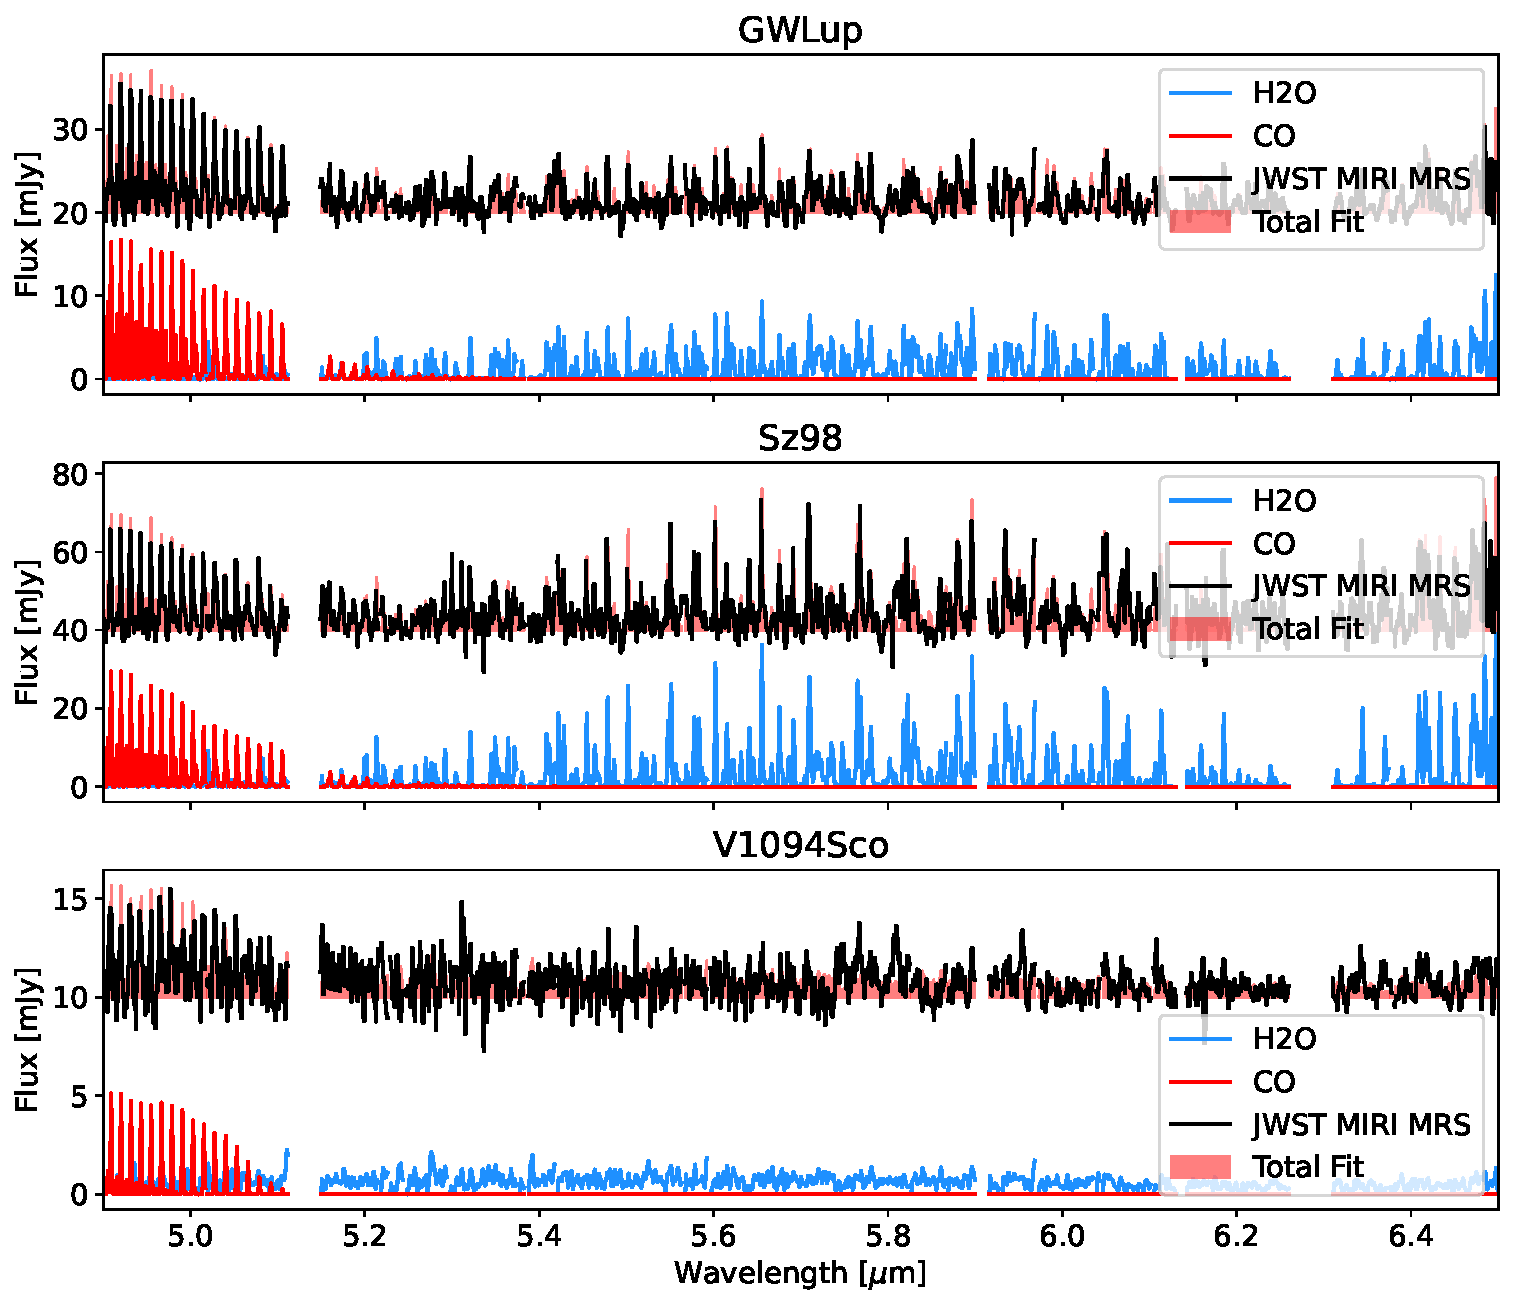
\includegraphics[width=\linewidth]{Figures/Fits.pdf}
    \caption{The fitted H\2O and CO spectra using a LTE model between 4.9 \textmu m and 6.5\textmu m for GWLup, Sz98, and V1094Sco}
    \label{fig: fits}
\end{figure}

Thereafter, the fitted CO and H\2O emission was removed from the spectra, and we applied the cross-correlation technique to the residuals of the spectrum. In GWLup and Sz98, no NO was detected. However, V1094Sco has a detection of NO. The residuals of GWLup, Sz98, and V1094Sco and the scaled NO templates are shown in \autoref{fig: no detect}. 

\begin{figure}[H]
    \centering
    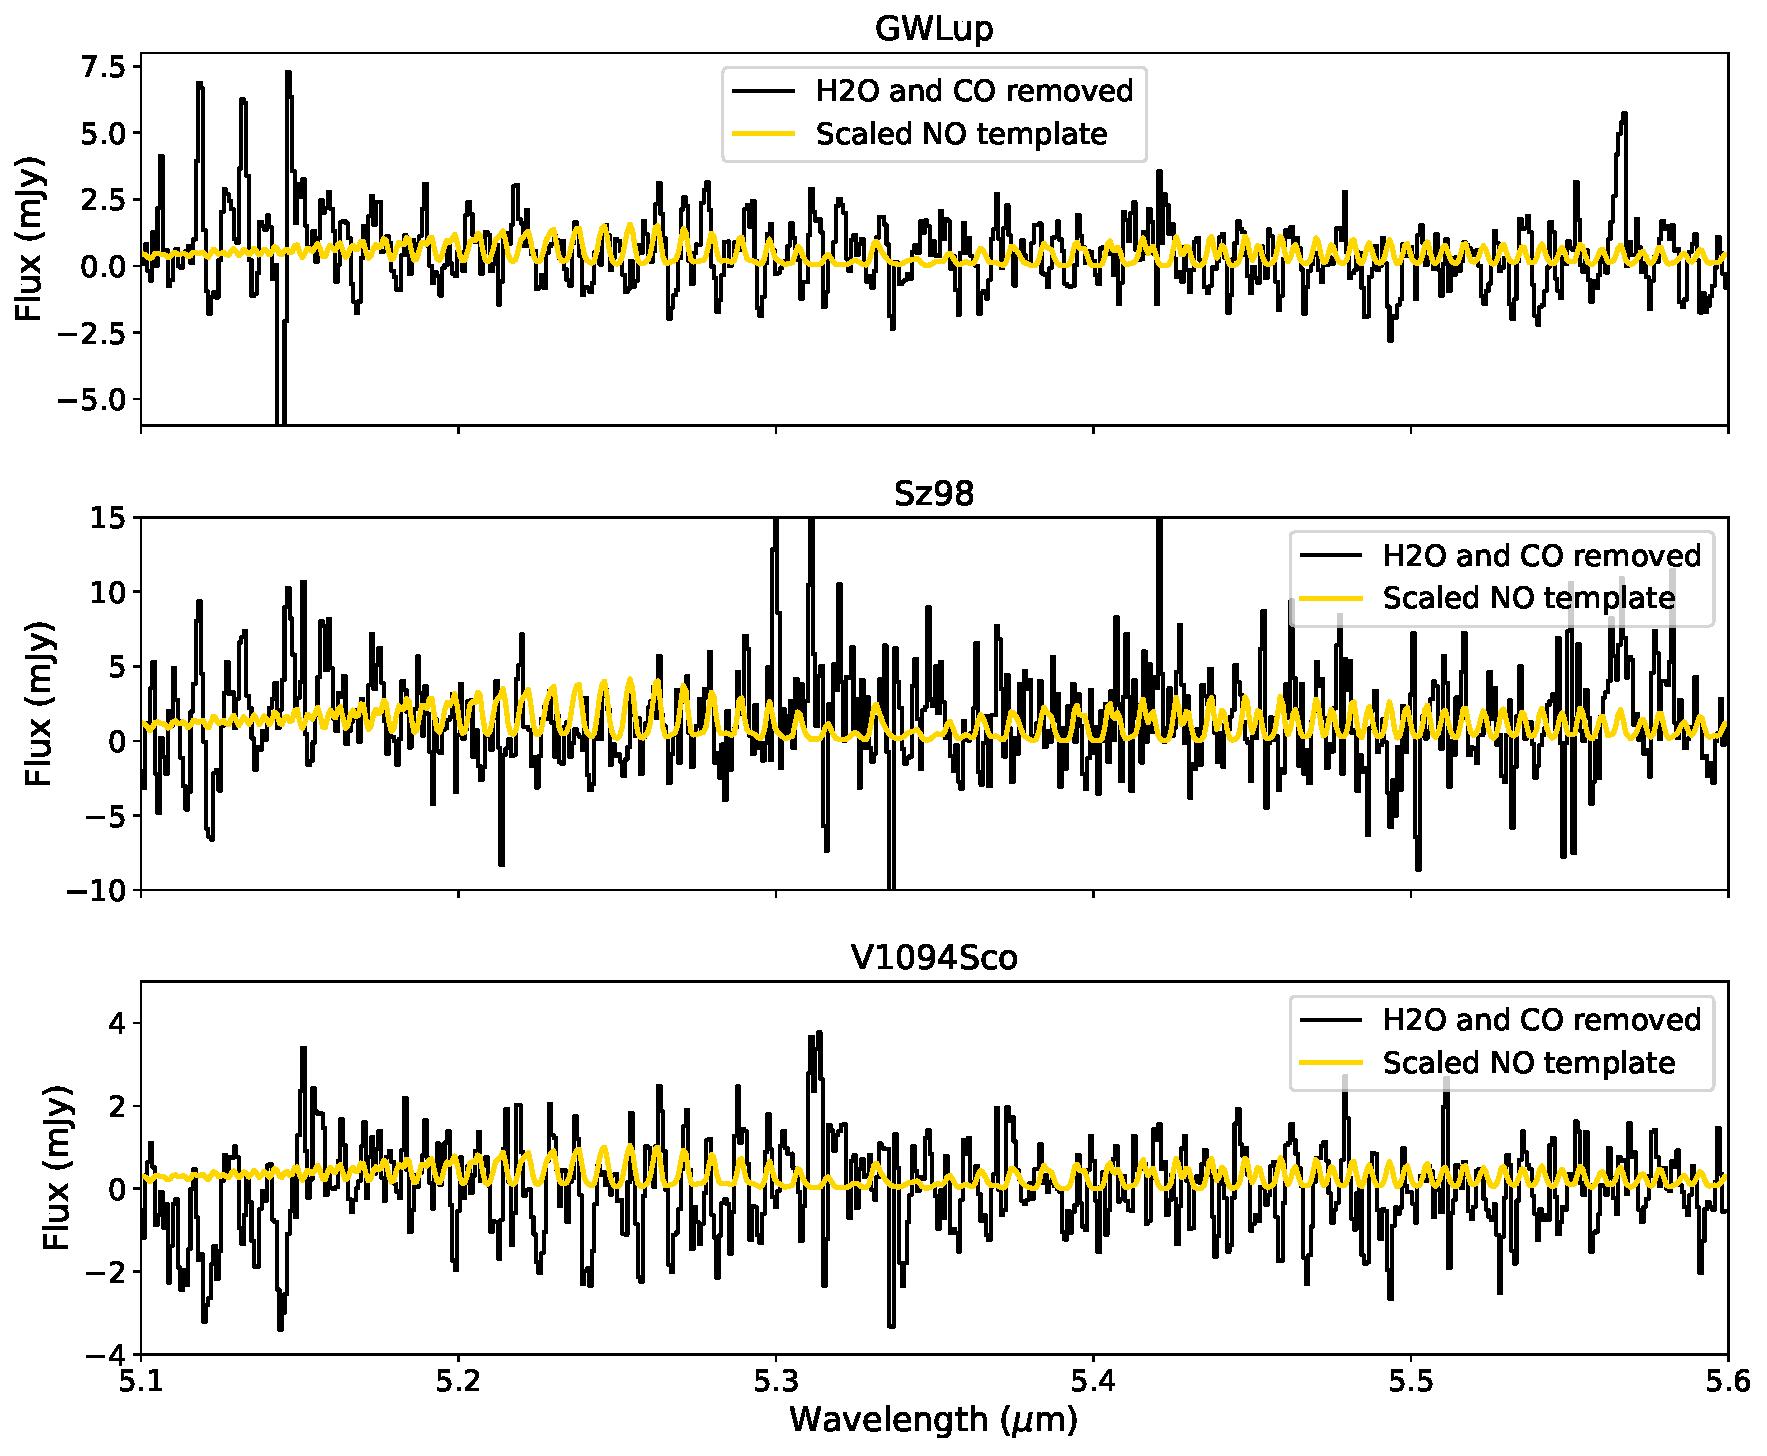
\includegraphics[width=\linewidth]{Figures/NO_Detect_stacked.pdf}
    \caption{The fitted H\2O and CO spectra using a LTE model between 4.9 \textmu m and 6.5\textmu m for V1094Sco}
    \label{fig: no detect}
\end{figure}

For all the residuals shown in \autoref{fig: no detect}, the NO emission is not clear in the residuals. However, in the region between 5.2 \textmu m and 5.3 \textmu m, the location of the peaks does align, especially for V1094Sco.

\subsection{Upper Limits on NH\3 and NO}
After subtracting the CO and H\2O emission from the spectra in the region between 4.9 \textmu m and 6.5 \textmu m, the only emission remaining is that of NO and NH\3. This was used to calculate the $\chi^2$ for different values of column density and temperature. This value can then be used to find the likelihood distribution. To update the prior, the temperature of the emitting regions of NO and NH\3 in the fiducial model was used (\autoref{fig: NONH3temp}).

\begin{figure}[H]
    \centering
    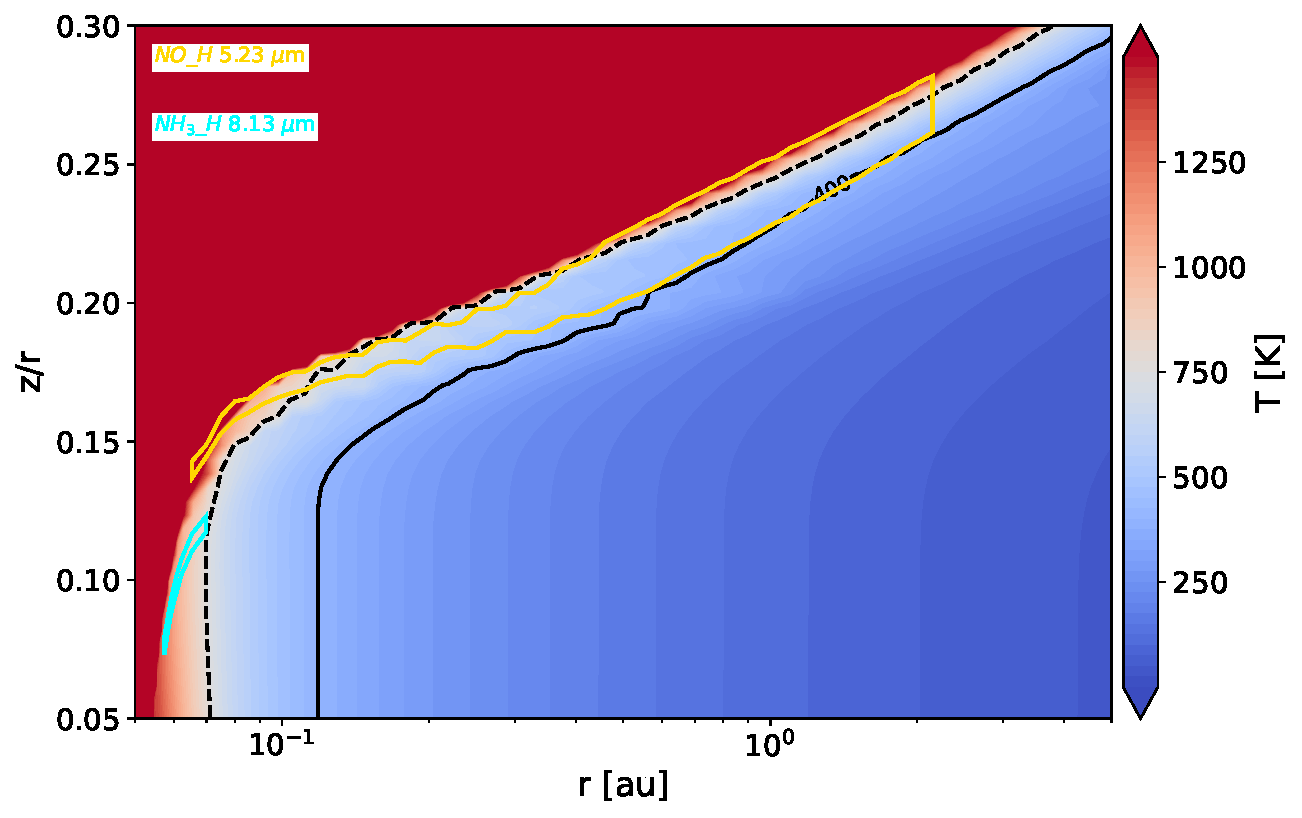
\includegraphics[width=\linewidth]{Figures/NONH3temp.pdf}
    \caption{The temperature of the gas across the disk. The emitting region of NH\3 is highlighted in cyan, and the emitting region of NO is highlighted in gold. The black contour lines show 400 K and 750 K. The emitting region of NO is outside the 400 K contour, meaning that its temperature is at least 400 K. Similarly, the emitting region of NH\3 is outside the 750 K contour, meaning that its temperature is at least 750 K.}
    \label{fig: NONH3temp}
\end{figure}

Using this, we concluded that the minimum temperature of NO is 400 K and of NH\3 750 K. These values were filled into the prior

\begin{equation}
    P(model) = 
    \begin{cases}
        1, & \text{if } T > T_0 \\
        0, & \text{if } T \leq T_0
    \end{cases}
\end{equation}

where $T_o=400$ K for NO and $T_o=750$ K for NH\3. Multiplying the prior with the likelihood distribution gave the posterior distribution up to a normalization constant, which was found by integrating the posterior distribution over all values of $N$ and $T$ and setting that equal to one. 10000 samples were drawn from the posterior distribution, and the number density values below which 95\% of the values fall are shown in \autoref{tab: upper limits}.

\begin{table}[H]
\begin{tabular}{lll}
\hline
Source   & NO ($\log(\mathrm{N})[\mathrm{cm}^{-2}])$   & NH\3 ($\log(\mathrm{N}) [\mathrm{cm}^{-2}])$\\ \hline
GWLup    & 16.5 & 21.1               \\
Sz98     & 17   & 20.2               \\
V1094Sco & 16.7 & 21.6               \\ \hline
\end{tabular}
\caption{The upper limits on the column density of NO and NH\3 for GWLup, Sz98, and V1094Sco}
\label{tab: upper limits}
\end{table}

\textbf{PLOT UPPER LIMITS}

\chapter{Discussion}\label{Ch: Discussion}
In this chapter, we discuss our results. First, we explain the interpretation of the results. Thereafter, we compare the molecules detected in the observations to the papers that provided the data, and compare our results to \cite{groningenthesis}. Next, we discuss the limitations of the simulations and the cross-correlation technique. Lastly, we present several improvements and ideas that other work could build on.
\section{Interpretation}
This thesis provides new insights into the detection of nitrogen carriers NO and NH\3 in the planet-forming regions of protoplanetary disks. The influence of C and O abundances on the spectra was analyzed. The spectra formed two groups: spectra dominated by H\2O emission for the models that have a C/O ratio smaller than one, and spectra dominated by C\2H\2 emission for models with C/O greater than one. Following this, emission of both NO and NH\3 was less obscured by water lines in the spectra of the carbon-rich models (see \autoref{fig: NO region}, \autoref{fig: NH3 region 1}, and \autoref{fig: NH3 region 2}), which leads to the conclusion that carbon-rich sources are the most prominent sources for the detection of NO and NH\3 in the planet-forming regions of protoplanetary disks. 

However, a direct NO and NH\3 detection from the spectrum proves to be difficult due to the low intensity of the emission of these molecules and the level of noise. To address this difficulty, we have tested a method using cross-correlation to detect weak spectral features. Using this technique on the simulated spectra generated using FLiTs resulted in no false positives. The most prominent features were detected in the spectrum, but not the weak emission from NO and NH\3. NO emission was detected in the spectrum of all the models after removing the emission of all other molecules for 10000 different random noises. However, only in 23.8\% of the spectra was the emission of NH\3 detected. Thus, NO is less difficult to detect in spectra.


\section{Comparison to Other Works}
\cite{Grant_2023} have detected CO, CO\2, H\2O, HCN, C\2H\2 and OH in the spectrum of GWLup. When we analyzed their spectrum with the cross-correlation technique, we detected the same molecules. Similarly, \cite{Gasman_2023} has detected CO, H\2O, OH, CO\2, and HCN in the spectrum of Sz98. Again, these are the same molecules we detected using the cross-correlation technique. The fact that we have the same results as they is a promising sign for the validity of our technique. 

\cite{groningenthesis} performed research similar to our own. However, they investigated the detection of SO\2 to learn more about the sulfur depletion problem. \textbf{MORE TEXT COMPARING OUR RESULTS}

\section{Limitations}
For the cross-correlation technique, we assume that the peak at lag=0 is purely from the molecule that is being tested. However, it could be the case that the cross-correlation of the noise with the template results in a peak, because the noise coincidentally follows a similar structure to the emission of the species. We suspect that this is highly unlikely, as the noise would then need to be in the same location (i.e., not shifted to different wavelengths) and follow a similar pattern (i.e., be bright in the same locations as the molecular emission). 

A problem that might be more impactful is fringing. Fringing is an interference effect that results in oscillations in spectra. This pattern could coincide with the pattern formed by the ro-vibrational transitions, which also has a regular spacing. If it were the case that these two phenomena would overlap, that could result in a false-positive.

Other than noise, other species could also interfere with our method of cross-correlation. When the emission of different spectra overlaps, that could result in a detection. For example, in \autoref{fig: NO region} the CO emission partly overlaps with the emission coming from NO. This, with the fact that the spacing of the two species is similar, could result in false positives when some CO emission is not removed. 

Following this, we use bootstrapping to create the hypothesis test by sampling the distribution of the test statistic. However, this destroys all patterns in the data. This can give a disproportionate view of the significance of a species' presence, leading to a false-positive.

Averaging the emission of all species across the entire grid may not be the best technique for creating a template. The different abundances heavily impact the shape of the emission, and combining them into a single template results in a spectrum that has about the same shape, but can lose 

\section{Future Work}
In this work, the only things that were varied were the C and O abundances. Some other properties could be interesting to investigate, for example, different disk structures. The distribution of NH\3 in \autoref{fig: nitrogen distribution} is close to the midplane in the disk, resulting in it being hidden inside the disk. Different disk structures, such as gaps, could expose the NH\3 reservoir, allowing for detection. In combination with observations by e.g., ALMA, this can narrow down the number of sources that can provide the first detection of NO or NH\3.

Furthermore, the stellar properties could affect the nitrogen carriers in the disk. Changing attributes such as stellar luminosity, mass, and temperature can result in different chemistries in the disk, thereby altering the spectrum that is measured. This can provide new insights into what properties are the most important to allow for detection of NO and NH\3. With that new information, possible objects of interest can be selected for observations. 

In \autoref{sec: flits}, we showed that sources with a C/O ratio greater than one have the highest potential for detection of NO and NH\3. \cite{Arabhavi_2024} showed that very low mass stars (VLMS) have high C/O ratios. Therefore, VLMS can prove to be promising sources for NO and NH\3 detection. 

\chapter{Conclusions}\label{Ch: Conclusions}
In this thesis, we have looked at the influence of the carbon and oxygen abundances on the nitrogen carriers in a protoplanetary disk and applied that knowledge to JWST MIRI MRS observations. Our main findings are as follows:
\begin{itemize}
    \item We showed that the total flux of NO increases as the C/O ratio decreases and NH\3 flux increases for lower C abundance. However, due to H\2O lines NO and NH\3 emission is difficult to detect in spectra of sources with a C/O ratio smaller than one. Therefore, the most promising sources for NO and NH\3 detection have a C/O ratio greater than one.
    \item We have selected spectral regions in which the emission from NO and NH\3 is the strongest. In particular, sources with a C/O ratio greater than one have the greatest potential for detecting NO and NH\3 as their emission is not obscured by H\2O emission.
    \item We tested a molecule detection method using cross-correlation. Using the ProDiMo models in the grid, emission templates were created for each species. 
    \item We reconfirmed the known species present in the spectra of GWLup, Sz98, and V1094Sco using the cross-correlation technique.
    \item We made a possible detection of NO in the spectrum of V1094Sco.
    \item We determined upper limits on the column densities of NO and NH\3 for GWLup, Sz98, and V1094Sco.
\end{itemize}
\textbf{SOMETHING ABOUT THE FUTURE}

\section*{Acknowledgements}
I would like to thank Marissa and Aditya for guiding me through this project, helping me understand topics, pitching new ideas, and giving feedback on my work. You definitely made this project really enjoyable and a great success. I would also like to thank Gerben and Luka for reading and giving feedback on my thesis; the figures and text would not have looked this good without you.

\bibliographystyle{aa.bst}
\bibliography{references}


\appendix
\chapter{More ProDiMo Results}
\begin{figure}
    \centering
    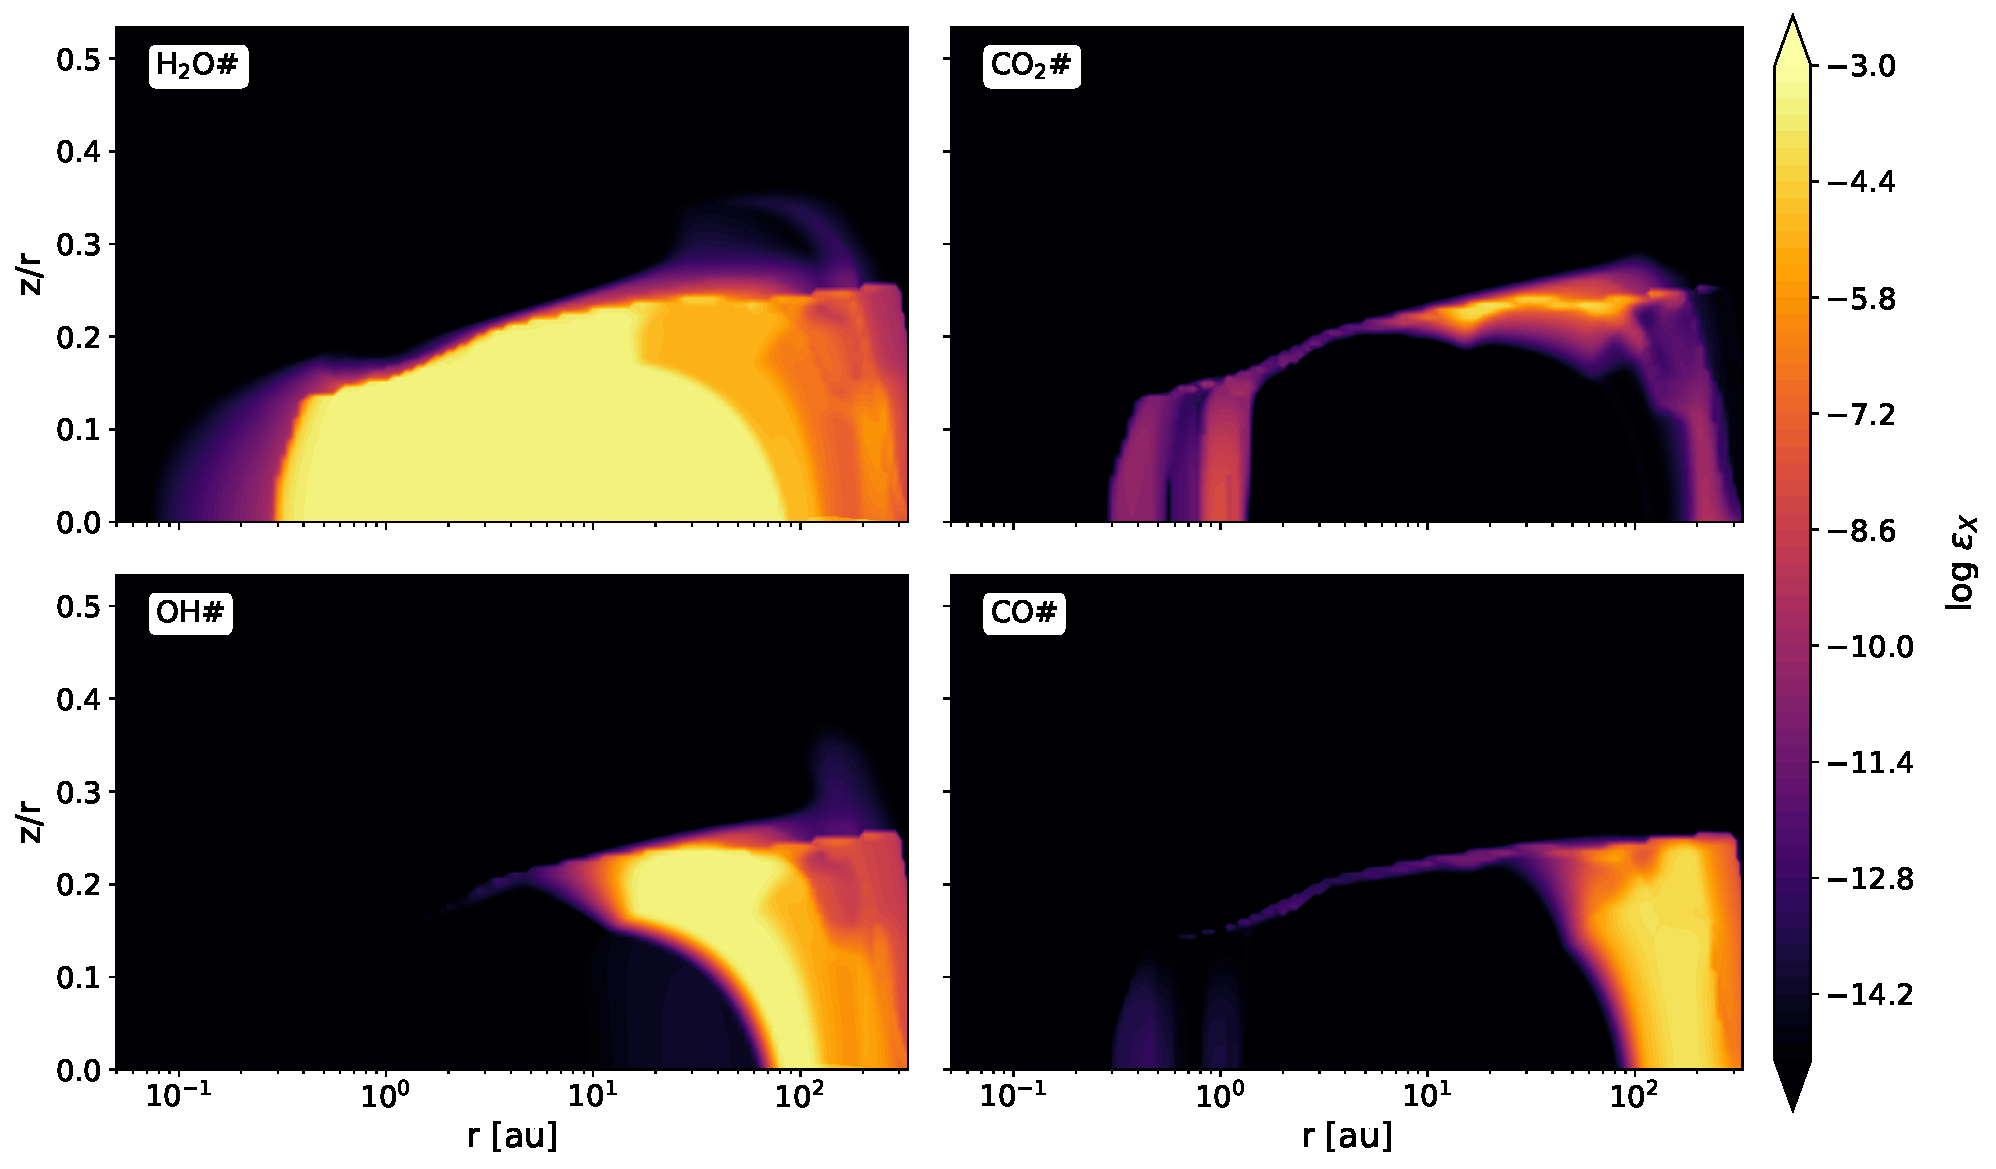
\includegraphics[width=\linewidth]{Figures/Abundance1ice.pdf}
    \caption{The distribution of H\2O, CO\2, OH, and CO ice across the disk of the fiducial model. The '#' denotes that the molecules are in the solid phase. The horizontal axis shows the distance $r$ from the host star, and the vertical axis shows the height above the midplane $z$ divided by the radius $r$.}
    \label{fig:enter-label}
\end{figure}
\begin{figure}
    \centering
    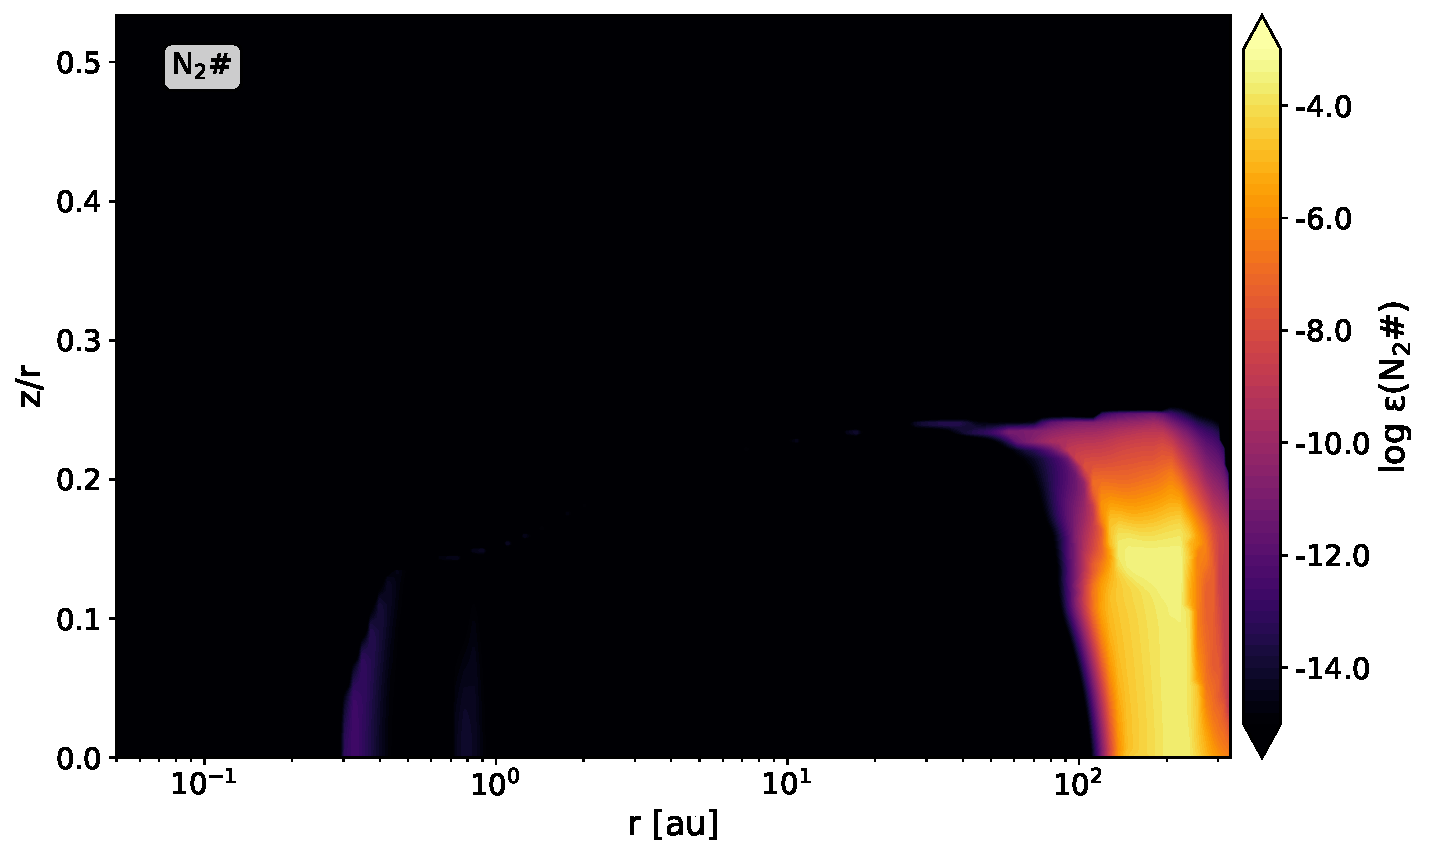
\includegraphics[width=\linewidth]{Figures/AbundanceN2ice.pdf}
    \caption{The distribution of N\2 ice across the disk of the fiducial model. The '#' denotes that the molecule is in the solid phase. The horizontal axis shows the distance $r$ from the host star, and the vertical axis shows the height above the midplane $z$ divided by the radius $r$.}
    \label{fig:enter-label}
\end{figure}
\begin{figure}
    \centering
    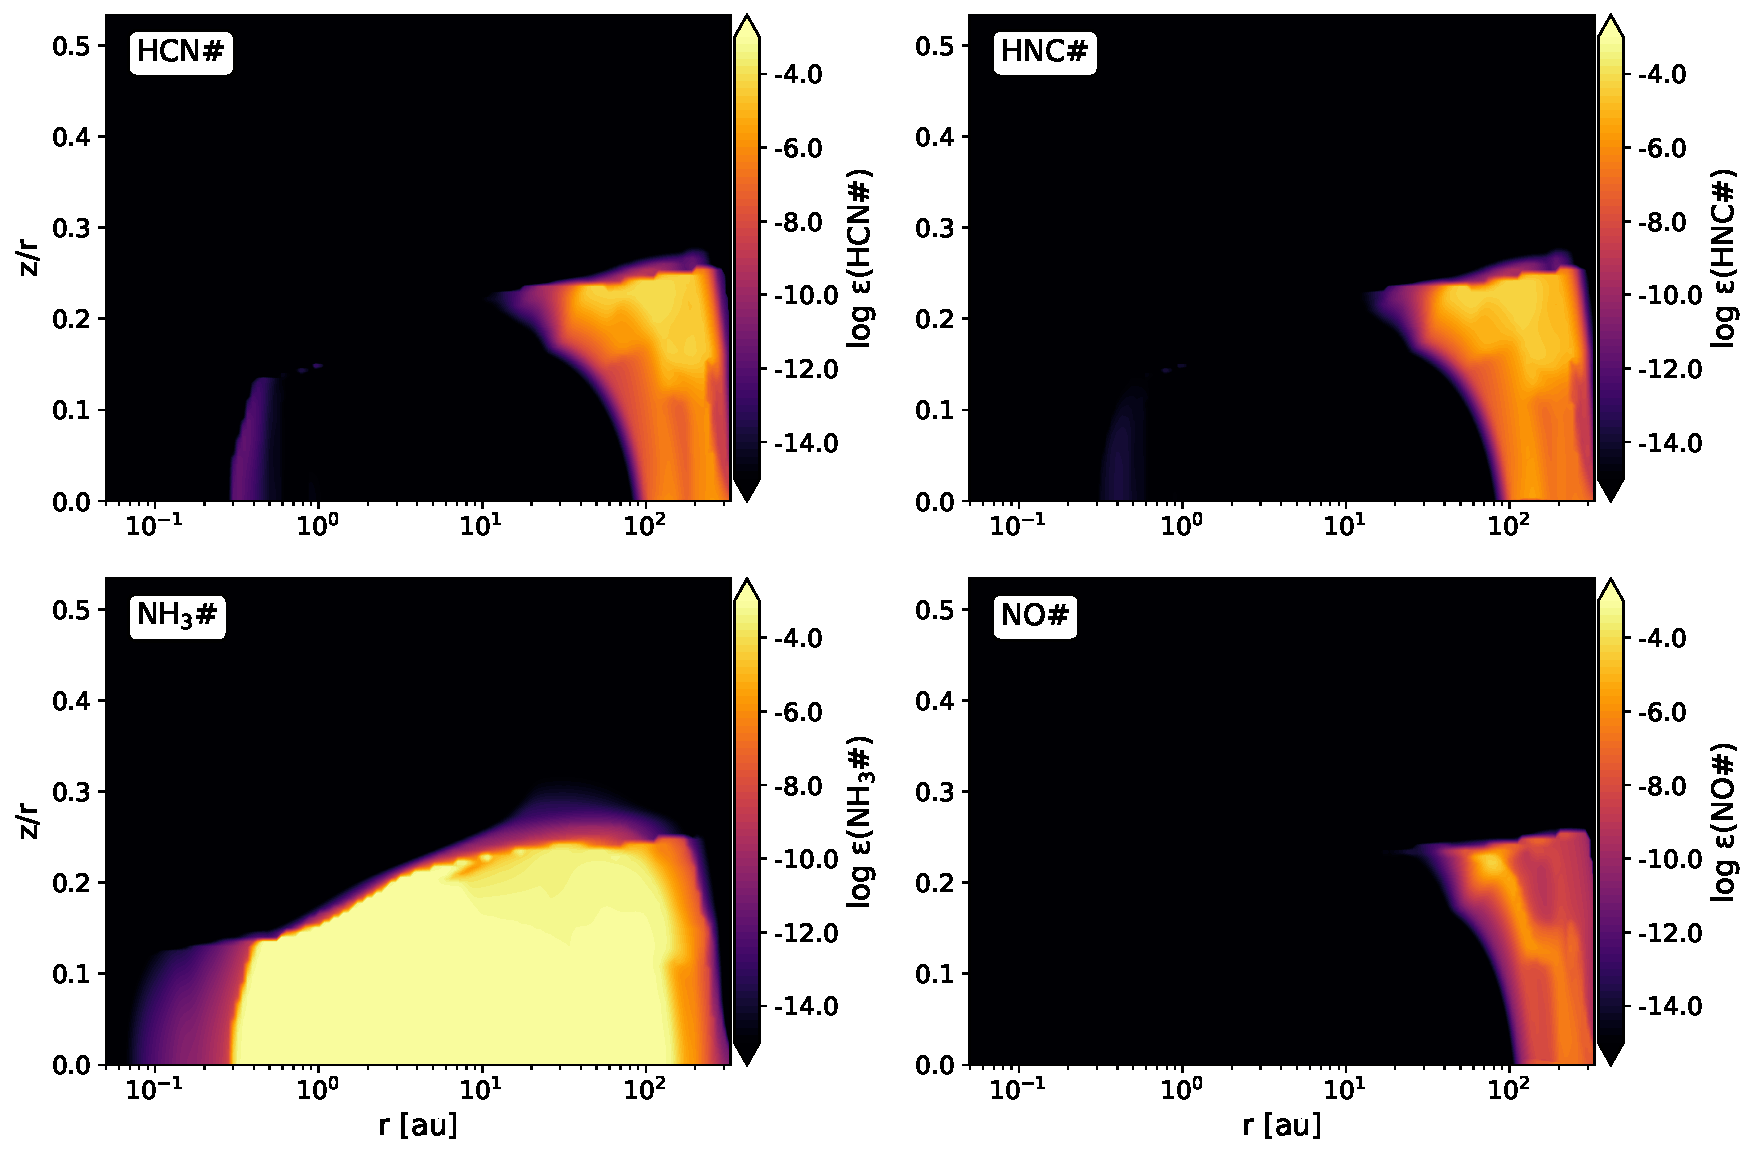
\includegraphics[width=\linewidth]{Figures/Abundance2ice.pdf}
    \caption{The distribution of HCN, HNC, NH\3, and NO ice across the disk of the fiducial model. The '#' denotes that the molecules are in the solid phase. The horizontal axis shows the distance $r$ from the host star, and the vertical axis shows the height above the midplane $z$ divided by the radius $r$.}
    \label{fig:enter-label}
\end{figure}



\chapter{Chi square fits}\label{app: chi square}
\begin{figure}[!ht]
    \centering
    \begin{subfigure}[b]{0.49\textwidth}
        \centering
        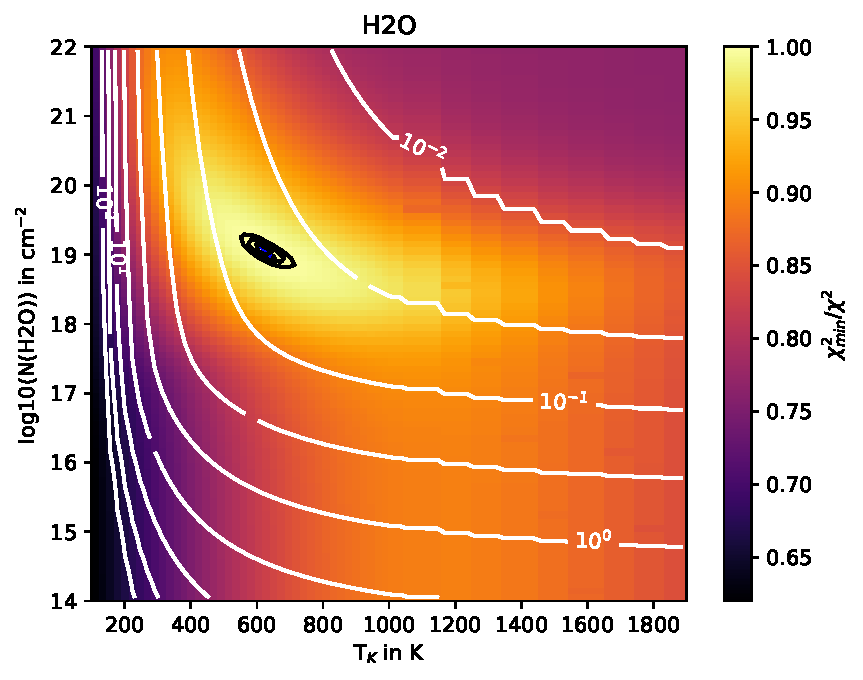
\includegraphics[width=\textwidth]{radexpy_niels/Radexpy_for_Niels/chi2_map_H2O_GWLup.pdf}
    \end{subfigure}
    \hfill
    \begin{subfigure}[b]{0.49\textwidth}
        \centering
        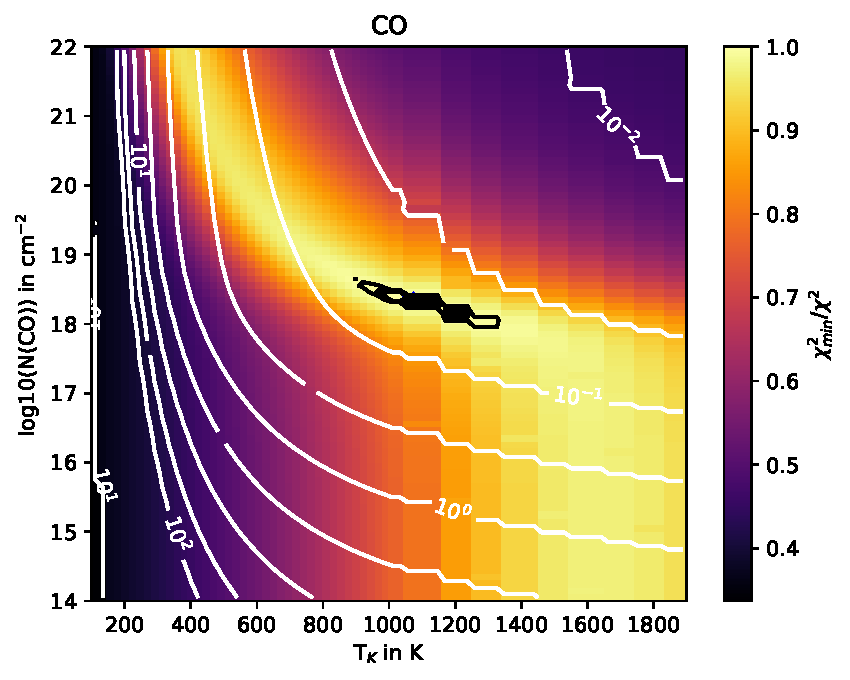
\includegraphics[width=\textwidth]{radexpy_niels/Radexpy_for_Niels/chi2_map_CO_GWLup.pdf}
    \end{subfigure}
    \caption{The $\chi^2$ heatmaps for fitting the H\2O and CO emission to the observation of GWLup. On the horizontal axis, the temperature in K is varied, and the column density is varied in orders of magnitude on the vertical axis. The black contour lines represent the 1$\sigma$, 2$\sigma$, and 3$\sigma$ confidence intervals. The white contour lines denote the best fitting emitting radius $R_e$ in au.}
\end{figure}

\begin{figure}[!ht]
    \centering
    \begin{subfigure}[b]{0.49\textwidth}
        \centering
        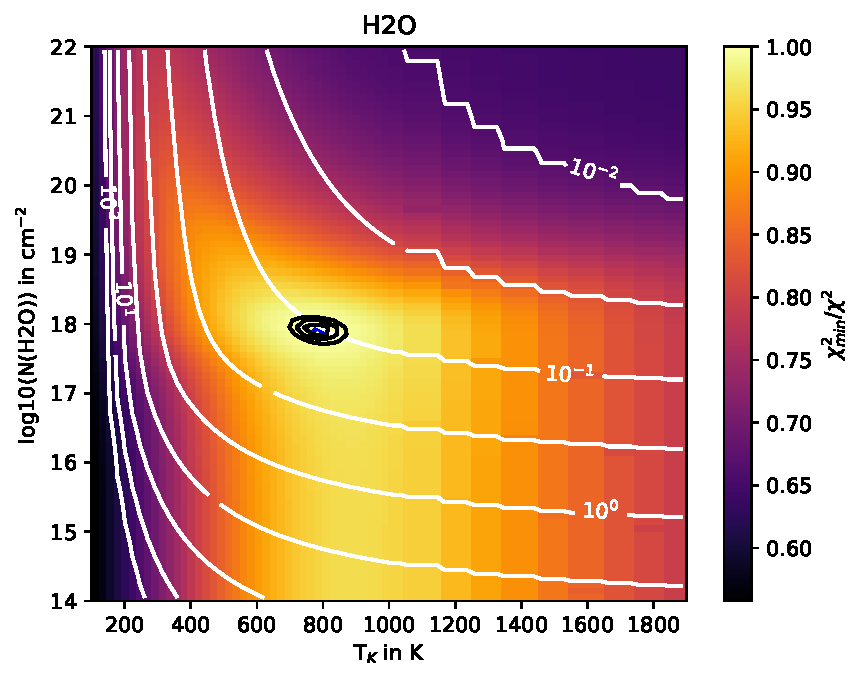
\includegraphics[width=\textwidth]{radexpy_niels/Radexpy_for_Niels/chi2_map_H2O_Sz98.pdf}
    \end{subfigure}
    \hfill
    \begin{subfigure}[b]{0.49\textwidth}
        \centering
        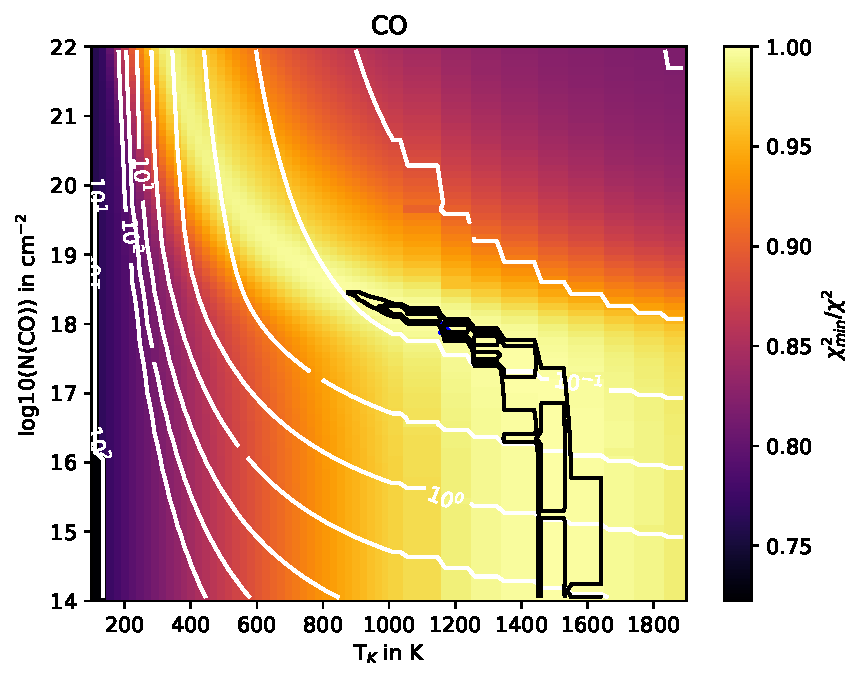
\includegraphics[width=\textwidth]{radexpy_niels/Radexpy_for_Niels/chi2_map_CO_Sz98.pdf}
    \end{subfigure}
    \caption{The $\chi^2$ heatmaps for fitting the H\2O and CO emission to the observation of GWLup. On the horizontal axis, the temperature in K is varied, and the column density is varied in orders of magnitude on the vertical axis. The black contour lines represent the 1$\sigma$, 2$\sigma$, and 3$\sigma$ confidence intervals. The white contour lines denote the best fitting emitting radius $R_e$ in au.}
\end{figure}

\begin{figure}[!ht]
    \centering
    \begin{subfigure}[b]{0.49\textwidth}
        \centering
        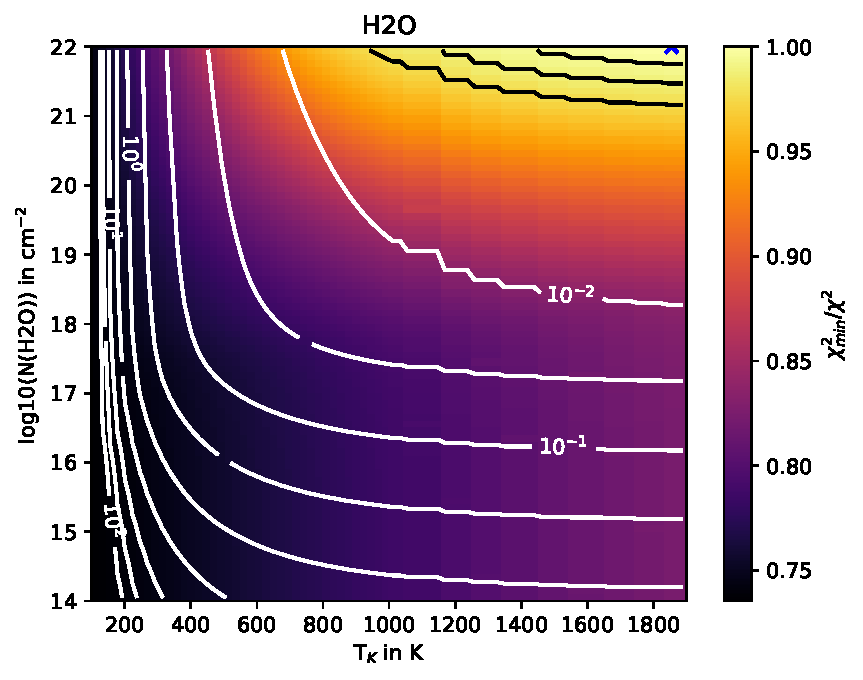
\includegraphics[width=\textwidth]{radexpy_niels/Radexpy_for_Niels/chi2_map_H2O_V1094Sco.pdf}
    \end{subfigure}
    \hfill
    \begin{subfigure}[b]{0.49\textwidth}
        \centering
        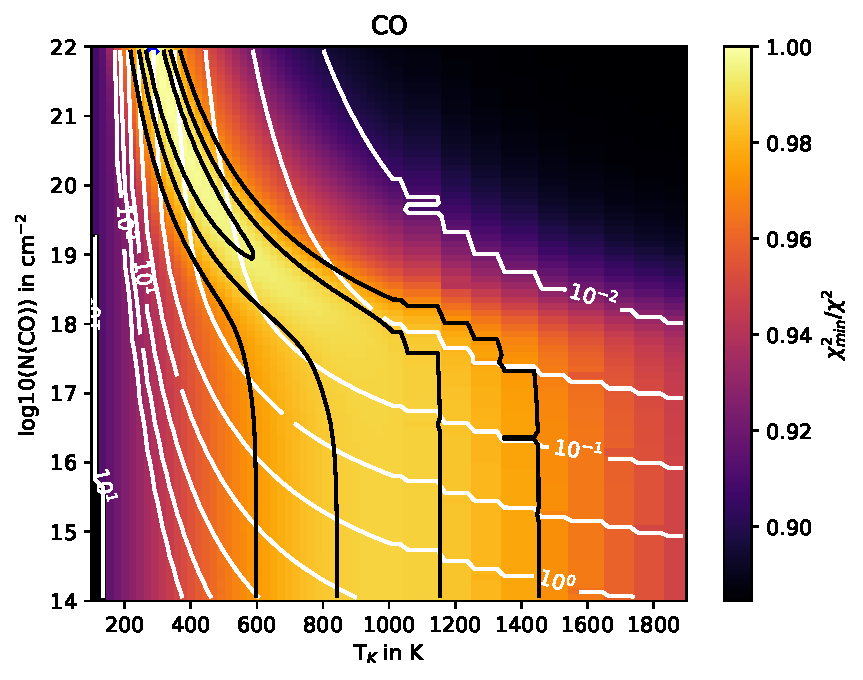
\includegraphics[width=\textwidth]{radexpy_niels/Radexpy_for_Niels/chi2_map_CO_V1094Sco.pdf}
    \end{subfigure}
    \caption{The $\chi^2$ heatmaps for fitting the H\2O and CO emission to the observation of V1094Sco. On the horizontal axis, the temperature in K is varied, and the column density is varied in orders of magnitude on the vertical axis. The black contour lines represent the 1$\sigma$, 2$\sigma$, and 3$\sigma$ confidence intervals. The white contour lines denote the best fitting emitting radius $R_e$ in au.}
\end{figure}
\chapter{Upper Limits}
\begin{figure}[!ht]
    \centering
    \begin{subfigure}[b]{0.49\textwidth}
        \centering
        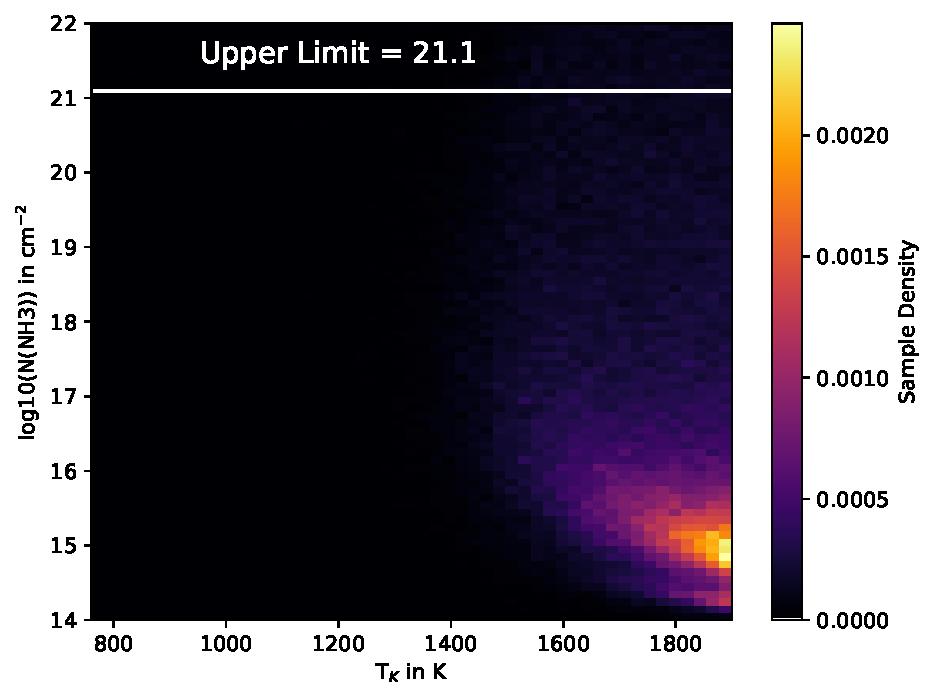
\includegraphics[width=\textwidth]{radexpy_niels/Radexpy_for_Niels/upper_NH3_GWLup.pdf}
    \end{subfigure}
    \hfill
    \begin{subfigure}[b]{0.49\textwidth}
        \centering
        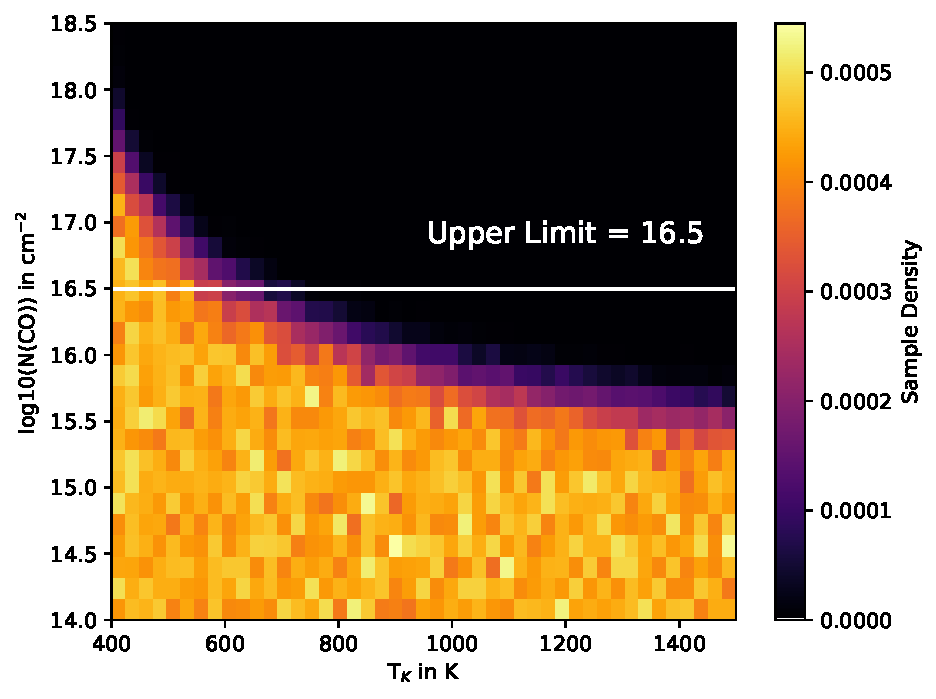
\includegraphics[width=\textwidth]{upper_CO_GWLup.pdf}
    \end{subfigure}
    \caption{The density distribution found by sampling the posterior distribution for the observation of GWLup. On the left is the density distribution for NH\3 is shown in the left panel, and the right panel shows the density distribution for NO. On the horizontal axis, the temperature in K is varied, and the column density is varied in orders of magnitude on the vertical axis. The white line is the upper limit on the column density and is defined as the column density below which 95\% of the density distribution falls.}
\end{figure}
\begin{figure}[!ht]
    \centering
    \begin{subfigure}[b]{0.49\textwidth}
        \centering
        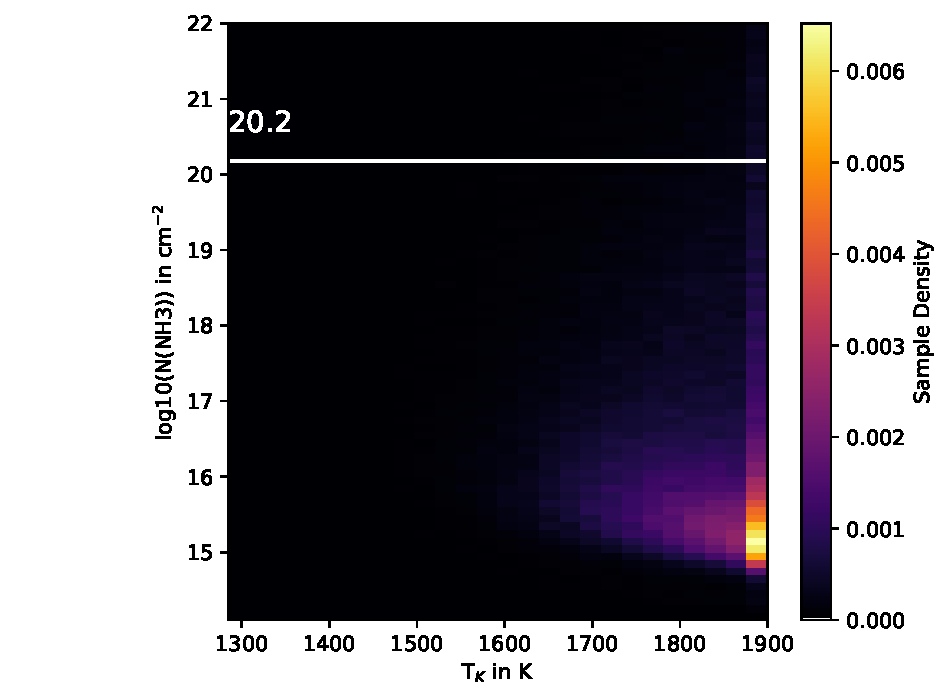
\includegraphics[width=\textwidth]{radexpy_niels/Radexpy_for_Niels/upper_NH3_Sz98.pdf}
    \end{subfigure}
    \hfill
    \begin{subfigure}[b]{0.49\textwidth}
        \centering
        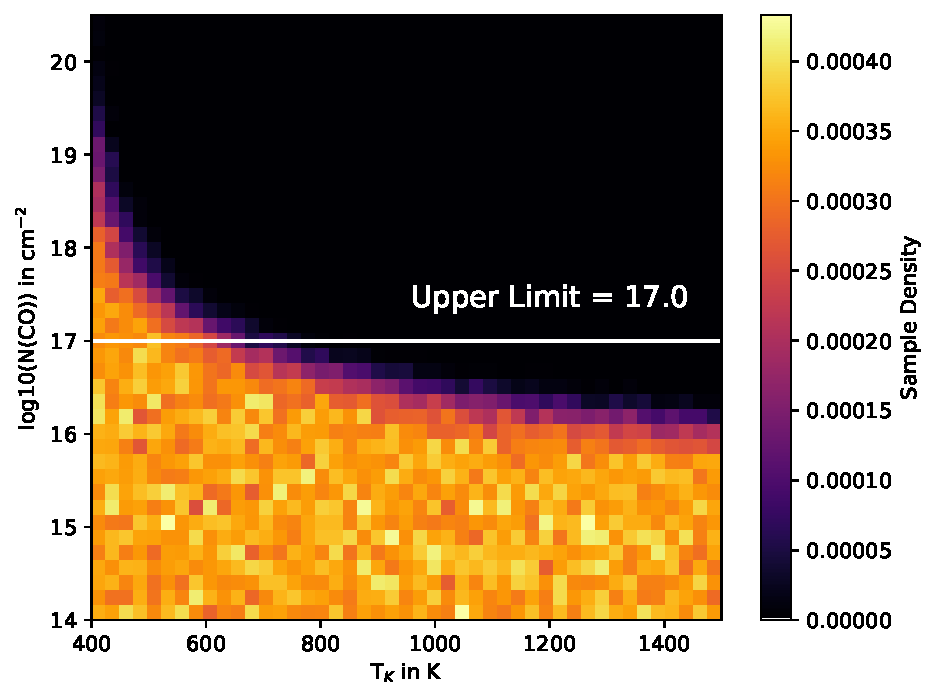
\includegraphics[width=\textwidth]{upper_CO_Sz98.pdf}
    \end{subfigure}
    \caption{The density distribution found by sampling the posterior distribution for the observation of Sz98. On the left is the density distribution for NH\3 is shown in the left panel, and the right panel shows the density distribution for NO. On the horizontal axis, the temperature in K is varied, and the column density is varied in orders of magnitude on the vertical axis. The white line is the upper limit on the column density and is defined as the column density below which 95\% of the density distribution falls.}
\end{figure}
\begin{figure}[!ht]
    \centering
    \begin{subfigure}[b]{0.49\textwidth}
        \centering
        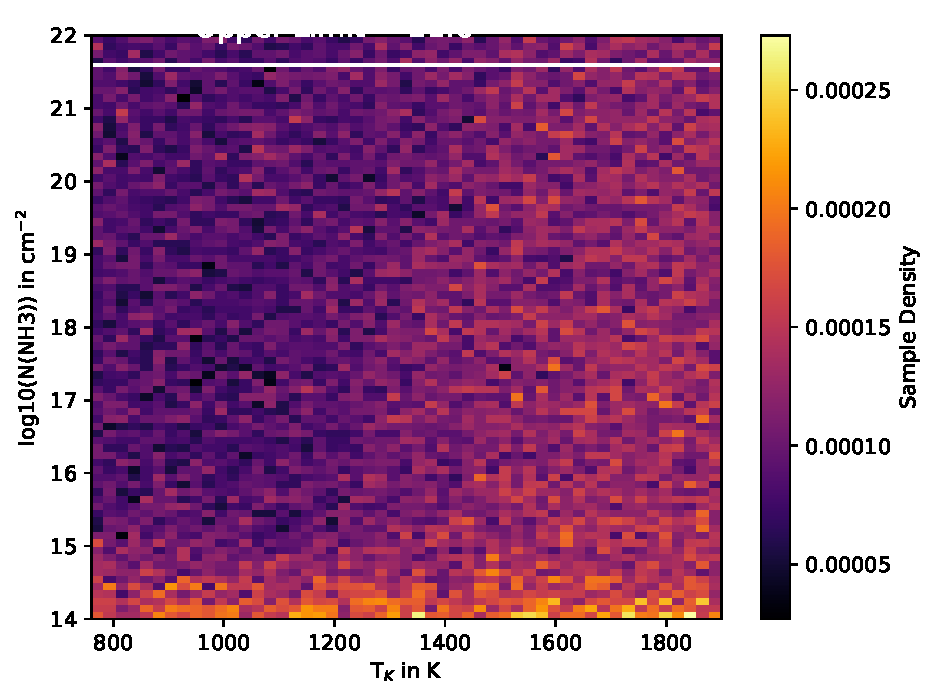
\includegraphics[width=\textwidth]{radexpy_niels/Radexpy_for_Niels/upper_NH3_V1094Sco.pdf}
    \end{subfigure}
    \hfill
    \begin{subfigure}[b]{0.49\textwidth}
        \centering
        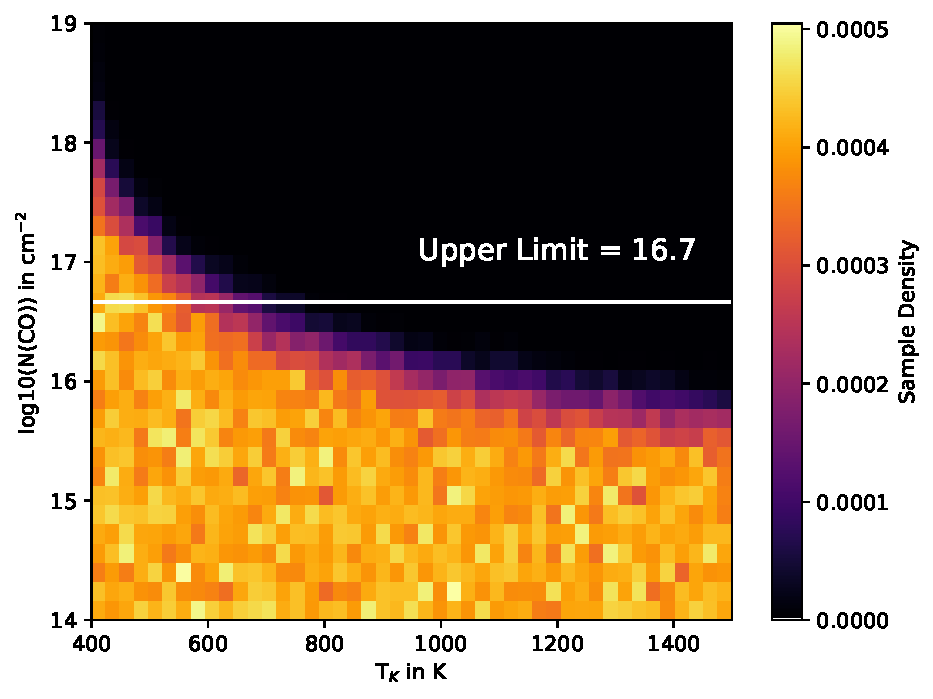
\includegraphics[width=\textwidth]{upper_CO_V1094Sco.pdf}
    \end{subfigure}
    \caption{The density distribution found by sampling the posterior distribution for the observation of V1094Sco. On the left is the density distribution for NH\3 is shown in the left panel, and the right panel shows the density distribution for NO. On the horizontal axis, the temperature in K is varied, and the column density is varied in orders of magnitude on the vertical axis. The white line is the upper limit on the column density and is defined as the column density below which 95\% of the density distribution falls.}
\end{figure}
\end{document}